% Options for packages loaded elsewhere
\PassOptionsToPackage{unicode}{hyperref}
\PassOptionsToPackage{hyphens}{url}
\PassOptionsToPackage{dvipsnames,svgnames,x11names}{xcolor}
%
\documentclass[
  11pt,
]{krantz}
\usepackage{amsmath,amssymb}
\usepackage{lmodern}
\usepackage{iftex}
\ifPDFTeX
  \usepackage[T1]{fontenc}
  \usepackage[utf8]{inputenc}
  \usepackage{textcomp} % provide euro and other symbols
\else % if luatex or xetex
  \usepackage{unicode-math}
  \defaultfontfeatures{Scale=MatchLowercase}
  \defaultfontfeatures[\rmfamily]{Ligatures=TeX,Scale=1}
  \setmonofont[Scale=0.775]{MesloLGS NF}
\fi
% Use upquote if available, for straight quotes in verbatim environments
\IfFileExists{upquote.sty}{\usepackage{upquote}}{}
\IfFileExists{microtype.sty}{% use microtype if available
  \usepackage[]{microtype}
  \UseMicrotypeSet[protrusion]{basicmath} % disable protrusion for tt fonts
}{}
\makeatletter
\@ifundefined{KOMAClassName}{% if non-KOMA class
  \IfFileExists{parskip.sty}{%
    \usepackage{parskip}
  }{% else
    \setlength{\parindent}{0pt}
    \setlength{\parskip}{6pt plus 2pt minus 1pt}}
}{% if KOMA class
  \KOMAoptions{parskip=half}}
\makeatother
\usepackage{xcolor}
\IfFileExists{xurl.sty}{\usepackage{xurl}}{} % add URL line breaks if available
\IfFileExists{bookmark.sty}{\usepackage{bookmark}}{\usepackage{hyperref}}
\hypersetup{
  pdftitle={Data Science per psicologi},
  pdfauthor={Corrado Caudek},
  colorlinks=true,
  linkcolor={Maroon},
  filecolor={Maroon},
  citecolor={Blue},
  urlcolor={Blue},
  pdfcreator={LaTeX via pandoc}}
\urlstyle{same} % disable monospaced font for URLs
\usepackage{color}
\usepackage{fancyvrb}
\newcommand{\VerbBar}{|}
\newcommand{\VERB}{\Verb[commandchars=\\\{\}]}
\DefineVerbatimEnvironment{Highlighting}{Verbatim}{commandchars=\\\{\}}
% Add ',fontsize=\small' for more characters per line
\usepackage{framed}
\definecolor{shadecolor}{RGB}{248,248,248}
\newenvironment{Shaded}{\begin{snugshade}}{\end{snugshade}}
\newcommand{\AlertTok}[1]{\textcolor[rgb]{0.33,0.33,0.33}{#1}}
\newcommand{\AnnotationTok}[1]{\textcolor[rgb]{0.37,0.37,0.37}{\textbf{\textit{#1}}}}
\newcommand{\AttributeTok}[1]{\textcolor[rgb]{0.61,0.61,0.61}{#1}}
\newcommand{\BaseNTok}[1]{\textcolor[rgb]{0.06,0.06,0.06}{#1}}
\newcommand{\BuiltInTok}[1]{#1}
\newcommand{\CharTok}[1]{\textcolor[rgb]{0.5,0.5,0.5}{#1}}
\newcommand{\CommentTok}[1]{\textcolor[rgb]{0.37,0.37,0.37}{\textit{#1}}}
\newcommand{\CommentVarTok}[1]{\textcolor[rgb]{0.37,0.37,0.37}{\textbf{\textit{#1}}}}
\newcommand{\ConstantTok}[1]{\textcolor[rgb]{0,0,0}{#1}}
\newcommand{\ControlFlowTok}[1]{\textcolor[rgb]{0.27,0.27,0.27}{\textbf{#1}}}
\newcommand{\DataTypeTok}[1]{\textcolor[rgb]{0.27,0.27,0.27}{#1}}
\newcommand{\DecValTok}[1]{\textcolor[rgb]{0.06,0.06,0.06}{#1}}
\newcommand{\DocumentationTok}[1]{\textcolor[rgb]{0.37,0.37,0.37}{\textbf{\textit{#1}}}}
\newcommand{\ErrorTok}[1]{\textcolor[rgb]{0.14,0.14,0.14}{\textbf{#1}}}
\newcommand{\ExtensionTok}[1]{#1}
\newcommand{\FloatTok}[1]{\textcolor[rgb]{0.06,0.06,0.06}{#1}}
\newcommand{\FunctionTok}[1]{\textcolor[rgb]{0,0,0}{#1}}
\newcommand{\ImportTok}[1]{#1}
\newcommand{\InformationTok}[1]{\textcolor[rgb]{0.37,0.37,0.37}{\textbf{\textit{#1}}}}
\newcommand{\KeywordTok}[1]{\textcolor[rgb]{0.27,0.27,0.27}{\textbf{#1}}}
\newcommand{\NormalTok}[1]{#1}
\newcommand{\OperatorTok}[1]{\textcolor[rgb]{0.43,0.43,0.43}{\textbf{#1}}}
\newcommand{\OtherTok}[1]{\textcolor[rgb]{0.37,0.37,0.37}{#1}}
\newcommand{\PreprocessorTok}[1]{\textcolor[rgb]{0.37,0.37,0.37}{\textit{#1}}}
\newcommand{\RegionMarkerTok}[1]{#1}
\newcommand{\SpecialCharTok}[1]{\textcolor[rgb]{0,0,0}{#1}}
\newcommand{\SpecialStringTok}[1]{\textcolor[rgb]{0.5,0.5,0.5}{#1}}
\newcommand{\StringTok}[1]{\textcolor[rgb]{0.5,0.5,0.5}{#1}}
\newcommand{\VariableTok}[1]{\textcolor[rgb]{0,0,0}{#1}}
\newcommand{\VerbatimStringTok}[1]{\textcolor[rgb]{0.5,0.5,0.5}{#1}}
\newcommand{\WarningTok}[1]{\textcolor[rgb]{0.37,0.37,0.37}{\textbf{\textit{#1}}}}
\usepackage{longtable,booktabs,array}
\usepackage{calc} % for calculating minipage widths
% Correct order of tables after \paragraph or \subparagraph
\usepackage{etoolbox}
\makeatletter
\patchcmd\longtable{\par}{\if@noskipsec\mbox{}\fi\par}{}{}
\makeatother
% Allow footnotes in longtable head/foot
\IfFileExists{footnotehyper.sty}{\usepackage{footnotehyper}}{\usepackage{footnote}}
\makesavenoteenv{longtable}
\usepackage{graphicx}
\makeatletter
\def\maxwidth{\ifdim\Gin@nat@width>\linewidth\linewidth\else\Gin@nat@width\fi}
\def\maxheight{\ifdim\Gin@nat@height>\textheight\textheight\else\Gin@nat@height\fi}
\makeatother
% Scale images if necessary, so that they will not overflow the page
% margins by default, and it is still possible to overwrite the defaults
% using explicit options in \includegraphics[width, height, ...]{}
\setkeys{Gin}{width=\maxwidth,height=\maxheight,keepaspectratio}
% Set default figure placement to htbp
\makeatletter
\def\fps@figure{htbp}
\makeatother
\setlength{\emergencystretch}{3em} % prevent overfull lines
\providecommand{\tightlist}{%
  \setlength{\itemsep}{0pt}\setlength{\parskip}{0pt}}
\setcounter{secnumdepth}{5}
\defaultfontfeatures{Scale=MatchLowercase}

\usepackage{booktabs}
\usepackage{longtable}
\usepackage[bf,singlelinecheck=off]{caption}

\usepackage{framed,color}
\definecolor{shadecolor}{RGB}{248,248,248}

\renewcommand{\textfraction}{0.05}
\renewcommand{\topfraction}{0.8}
\renewcommand{\bottomfraction}{0.8}
\renewcommand{\floatpagefraction}{0.75}

\renewenvironment{quote}{\begin{VF}}{\end{VF}}
\let\oldhref\href
\renewcommand{\href}[2]{#2\footnote{\url{#1}}}

\ifxetex
  \usepackage{letltxmacro}
  \setlength{\XeTeXLinkMargin}{1pt}
  \LetLtxMacro\SavedIncludeGraphics\includegraphics
  \def\includegraphics#1#{% #1 catches optional stuff (star/opt. arg.)
    \IncludeGraphicsAux{#1}%
  }%
  \newcommand*{\IncludeGraphicsAux}[2]{%
    \XeTeXLinkBox{%
      \SavedIncludeGraphics#1{#2}%
    }%
  }%
\fi

\makeatletter
\newenvironment{kframe}{%
\medskip{}
\setlength{\fboxsep}{.8em}
 \def\at@end@of@kframe{}%
 \ifinner\ifhmode%
  \def\at@end@of@kframe{\end{minipage}}%
  \begin{minipage}{\columnwidth}%
 \fi\fi%
 \def\FrameCommand##1{\hskip\@totalleftmargin \hskip-\fboxsep
 \colorbox{shadecolor}{##1}\hskip-\fboxsep
     % There is no \\@totalrightmargin, so:
     \hskip-\linewidth \hskip-\@totalleftmargin \hskip\columnwidth}%
 \MakeFramed {\advance\hsize-\width
   \@totalleftmargin\z@ \linewidth\hsize
   \@setminipage}}%
 {\par\unskip\endMakeFramed%
 \at@end@of@kframe}
\makeatother

\renewenvironment{Shaded}{\begin{kframe}}{\end{kframe}}

\usepackage{makeidx}
\makeindex

\urlstyle{tt}

\usepackage{amsthm}
\makeatletter
\def\thm@space@setup{%
  \thm@preskip=8pt plus 2pt minus 4pt
  \thm@postskip=\thm@preskip
}
\makeatother

\newcommand{\E}{\mathbb{E}} % Define expected value operator
\DeclareMathOperator{\Var}{\mathbb{V}} % Define variance operator
\DeclareMathOperator{\SD}{SD} % Define sd operator
\DeclareMathOperator{\Cov}{Cov} % Define covariance operator
\DeclareMathOperator{\Corr}{Corr} % Define correlation operator
\DeclareMathOperator{\Me}{Me} % Define mediane operator
\DeclareMathOperator{\Mo}{Mo} % Define mode operator
\DeclareMathOperator{\Bin}{Bin} % Define binomial operator
\DeclareMathOperator{\Bernoulli}{Bernoulli} % Define Bernoulli operator
\DeclareMathOperator{\Poi}{Poi} % Define Poisson operator
\DeclareMathOperator{\Uniform}{Uniform} % Define Uniform operator
\DeclareMathOperator{\Cauchy}{Cauchy} % Define Cauchy operator
\DeclareMathOperator{\elpd}{elpd} % Define elpd operator
\DeclareMathOperator{\lppd}{lppd} % Define lppd operator
\DeclareMathOperator{\LOO}{LOO} % Define LOO operator
\DeclareMathOperator{\Ber}{\mathscr{B}} % Define Bernoulli operator
\DeclareMathOperator{\B}{B} % beta function
% \mbox{B}(a, b) % beta function
% \mbox{Beta}(a, b) % beta distribution
\newcommand{\R}{\textsf{R}} % Define R programming language symbol
\newcommand{\Real}{\mathbb{R}} % Define real number operator
\newcommand{\Prob}{\mathscr{P}}
\DeclareMathOperator{\argmin}{arg\,min} % thin space, limits on side in displays
\DeclareMathOperator{\argmax}{arg\,max} % no space, limits on side in displays

\raggedbottom % allow variable (ragged) site heights
\frenchspacing

\usepackage[
 labelfont=bf,
 font={small, it}
]{caption}
\usepackage{upquote} % print correct quotes in verbatim-environments
\usepackage{empheq}
\usepackage{xfrac}

\usepackage{polyglossia}
\setmainlanguage{italian}

% \DeclareMathSizes{10}{9}{7}{5}

\frontmatter
\ifLuaTeX
  \usepackage{selnolig}  % disable illegal ligatures
\fi
\usepackage[]{natbib}
\bibliographystyle{apalike}

\title{Data Science per psicologi}
\author{Corrado Caudek}
\date{2022-01-17}

\usepackage{amsthm}
\newtheorem{theorem}{Teorema}[chapter]
\newtheorem{lemma}{Lemma}[chapter]
\newtheorem{corollary}{Corollario}[chapter]
\newtheorem{proposition}{Proposizione}[chapter]
\newtheorem{conjecture}{Congettura}[chapter]
\theoremstyle{definition}
\newtheorem{definition}{Definizione}[chapter]
\theoremstyle{definition}
\newtheorem{example}{Esempio}[chapter]
\theoremstyle{definition}
\newtheorem{exercise}{Esercizio}[chapter]
\theoremstyle{definition}
\newtheorem{hypothesis}{Hypothesis}[chapter]
\theoremstyle{remark}
\newtheorem*{remark}{Osservazione}
\newtheorem*{solution}{Soluzione}
\begin{document}
\maketitle

\cleardoublepage\newpage\thispagestyle{empty}\null
% \cleardoublepage\newpage\thispagestyle{empty}\null
%\cleardoublepage\newpage
\thispagestyle{empty}
\begin{center}
\Large{Psicometria -- AA 2021/2022}

\vskip20pt

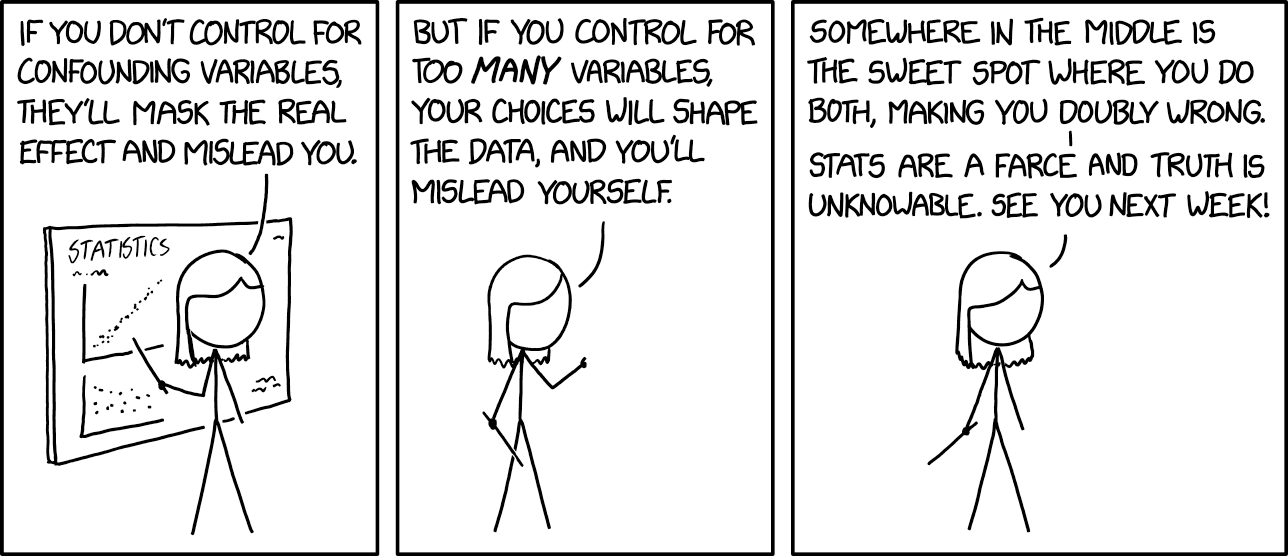
\includegraphics{images/confounding_variables.png}
\end{center}

\setlength{\abovedisplayskip}{-5pt}
\setlength{\abovedisplayshortskip}{-5pt}

{
\hypersetup{linkcolor=}
\setcounter{tocdepth}{2}
\tableofcontents
}
\listoffigures
\listoftables
\hypertarget{prefazione}{%
\chapter*{Prefazione}\label{prefazione}}


\emph{Data Science per psicologi} contiene il materiale delle lezioni dell'insegnamento di \emph{Psicometria B000286} (A.A. 2021/2022) rivolto agli studenti del primo anno del Corso di Laurea in Scienze e Tecniche Psicologiche dell'Università degli Studi di Firenze. \emph{Psicometria} si propone di fornire agli studenti un'introduzione all'analisi dei dati in psicologia. Le conoscenze/competenze che verranno sviluppate in questo insegnamento sono quelle della Data science, ovvero un insieme di conoscenze/competenze che si pongono all'intersezione tra statistica (ovvero, richiedono la capacità di comprendere teoremi statistici) e informatica (ovvero, richiedono la capacità di sapere utilizzare un software).

\hypertarget{la-psicologia-e-la-data-science}{%
\section*{La psicologia e la Data science}\label{la-psicologia-e-la-data-science}}


Sembra sensato spendere due parole su un tema che è importante per gli studenti: quello indicato dal titolo di questo Capitolo. È ovvio che agli studenti di psicologia la statistica non piace. Se piacesse, forse studierebbero Data science e non psicologia; ma non lo fanno. Di conseguenza, gli studenti di psicologia si chiedono: ``perché dobbiamo perdere tanto tempo a studiare queste cose quando in realtà quello che ci interessa è tutt'altro?'' Questa è una bella domanda.

C'è una ragione molto semplice che dovrebbe farci capire perché la Data science è così importante per la psicologia. Infatti, a ben pensarci, la psicologia è una disciplina intrinsecamente statistica, se per statistica intendiamo quella disciplina che studia la variazione delle caratteristiche degli individui nella popolazione. La psicologia studia \emph{gli individui} ed è proprio la variabilità inter- e intra-individuale ciò che vogliamo descrivere e, in certi casi, predire. In questo senso, la psicologia è molto diversa dall'ingegneria, per esempio. Le proprietà di un determinato ponte sotto certe condizioni, ad esempio, sono molto simili a quelle di un altro ponte, sotto le medesime condizioni. Quindi, per un ingegnere la statistica è poco importante: le proprietà dei materiali sono unicamente dipendenti dalla loro composizione e restano costanti. Ma lo stesso non può dirsi degli individui: ogni individuo è unico e cambia nel tempo. E le variazioni tra gli individui, e di un individuo nel tempo, sono l'oggetto di studio proprio della psicologia: è dunque chiaro che i problemi che la psicologia si pone sono molto diversi da quelli affrontati, per esempio, dagli ingegneri. Questa è la ragione per cui abbiamo tanto bisogno della Data science in psicologia: perché la Data science ci consente di descrivere la variazione e il cambiamento. E queste sono appunto le caratteristiche di base dei fenomeni psicologici.

Sono sicuro che, leggendo queste righe, a molti studenti sarà venuta in mente la seguente domanda: perché non chiediamo a qualche esperto di fare il ``lavoro sporco'' (ovvero le analisi statistiche) per noi, mentre noi (gli psicologi) ci occupiamo solo di ciò che ci interessa, ovvero dei problemi psicologici slegati dai dettagli ``tecnici'' della Data science? La risposta a questa domanda è che non è possibile progettare uno studio psicologico sensato senza avere almeno una comprensione rudimentale della Data science. Le tematiche della Data science non possono essere ignorate né dai ricercatori in psicologia né da coloro che svolgono la professione di psicologo al di fuori dell'Università. Infatti, anche i professionisti al di fuori dall'università non possono fare a meno di leggere la letteratura psicologica più recente: il continuo aggiornamento delle conoscenze è infatti richiesto dalla deontologia della professione. Ma per potere fare questo è necessario conoscere un bel po' di Data science! Basta aprire a caso una rivista specialistica di psicologia per rendersi conto di quanto ciò sia vero: gli articoli che riportano i risultati delle ricerche psicologiche sono zeppi di analisi statistiche e di modelli formali. E la comprensione della letteratura psicologica rappresenta un requisito minimo nel bagaglio professionale dello psicologo.

Le considerazioni precedenti cercano di chiarire il seguente punto: la Data science non è qualcosa da studiare a malincuore, in un singolo insegnamento universitario, per poi poterla tranquillamente dimenticare. Nel bene e nel male, gli psicologi usano gli strumenti della Data science in tantissimi ambiti della loro attività professionale: in particolare quando costruiscono, somministrano e interpretano i test psicometrici. È dunque chiaro che possedere delle solide basi di Data science è un tassello imprescindibile del bagaglio professionale dello psicologo. In questo insegnamento verrano trattati i temi base della Data science e verrà adottato un punto di vista bayesiano, che corrisponde all'approccio più recente e sempre più diffuso in psicologia.

\hypertarget{come-studiare}{%
\section*{Come studiare}\label{come-studiare}}


Il giusto metodo di studio per prepararsi all'esame di Psicometria è quello di seguire attivamente le lezioni, assimilare i concetti via via che essi vengono presentati e verificare in autonomia le procedure presentate a lezione. Incoraggio gli studenti a farmi domande per chiarire ciò che non è stato capito appieno. Incoraggio gli studenti a utilizzare i forum attivi su Moodle e, soprattutto, a svolgere gli esercizi proposti su Moodle. I problemi forniti su Moodle rappresentano il livello di difficoltà richiesto per superare l'esame e consentono allo studente di comprendere se le competenze sviluppate fino a quel punto sono sufficienti rispetto alle richieste dell'esame.

La prima fase dello studio, che è sicuramente individuale, è quella in cui è necessario acquisire le conoscenze teoriche relative ai problemi che saranno presentati all'esame. La seconda fase di studio, che può essere facilitata da scambi con altri e da incontri di gruppo, porta ad acquisire la capacità di applicare le conoscenze: è necessario capire come usare un software (\(\textsf{R}\)) per applicare i concetti statistici alla specifica situazione del problema che si vuole risolvere. Le due fasi non sono però separate: il saper fare molto spesso ci aiuta a capire meglio.

\hypertarget{sviluppare-un-metodo-di-studio-efficace}{%
\section*{Sviluppare un metodo di studio efficace}\label{sviluppare-un-metodo-di-studio-efficace}}


Avendo insegnato molte volte in passato un corso introduttivo di analisi dei dati ho notato nel corso degli anni che gli studenti con l'atteggiamento mentale che descriverò qui sotto generalmente ottengono ottimi risultati. Alcuni studenti sviluppano naturalmente questo approccio allo studio, ma altri hanno bisogno di fare uno sforzo per maturarlo. Fornisco qui sotto una breve descrizione del ``metodo di studio'' che, nella mia esperienza, è il più efficace per affrontare le richieste di questo insegnamento.

\begin{itemize}
\tightlist
\item
  Dedicate un tempo sufficiente al materiale di base, apparentemente facile; assicuratevi di averlo capito bene. Cercate le lacune nella vostra comprensione. Leggere presentazioni diverse dello stesso materiale (in libri o articoli diversi) può fornire nuove intuizioni.
\item
  Gli errori che facciamo sono i nostri migliori maestri. Istintivamente cerchiamo di dimenticare subito i nostri errori. Ma il miglior modo di imparare è apprendere dagli errori che commettiamo. In questo senso, una soluzione corretta è meno utile di una soluzione sbagliata. Quando commettiamo un errore questo ci fornisce un'informazione importante: ci fa capire qual è il materiale di studio sul quale dobbiamo ritornare e che dobbiamo capire meglio.
\item
  C'è ovviamente un aspetto ``psicologico'' nello studio. Quando un esercizio o problema ci sembra incomprensibile, la cosa migliore da fare è dire: ``mi arrendo'', ``non ho idea di cosa fare!''. Questo ci rilassa: ci siamo già arresi, quindi non abbiamo niente da perdere, non dobbiamo più preoccuparci. Ma non dobbiamo fermarci qui. Le cose ``migliori'' che faccio (se ci sono) le faccio quando non ho voglia di lavorare. Alle volte, quando c'è qualcosa che non so fare e non ho idea di come affontare, mi dico: ``oggi non ho proprio voglia di fare fatica'', non ho voglia di mettermi nello stato mentale per cui ``in 10 minuti devo risolvere il problema perché dopo devo fare altre cose''. Però ho voglia di \emph{divertirmi} con quel problema e allora mi dedico a qualche aspetto ``marginale'' del problema, che so come affrontare, oppure considero l'aspetto più difficile del problema, quello che non so come risolvere, ma invece di cercare di risolverlo, guardo come altre persone hanno affrontato problemi simili, opppure lo stesso problema in un altro contesto. Non mi pongo l'obiettivo ``risolvi il problema in 10 minuti'', ma invece quello di farmi un'idea ``generale'' del problema, o quello di capire un caso più specifico e più semplice del problema. Senza nessuna pressione. Infatti, in quel momento ho deciso di non lavorare (ovvero, di non fare fatica). Va benissimo se ``parto per la tangente'', ovvero se mi metto a leggere del materiale che sembra avere poco a che fare con il problema centrale (le nostre intuizioni e la nostra curiosità solitamente ci indirizzano sulla strada giusta). Quando faccio così, molto spesso trovo la soluzione del problema che mi ero posto e, paradossalmente, la trovo in un tempo minore di quello che, in precedenza, avevo dedicato a ``lavorare'' al problema. Allora perché non faccio sempre così? C'è ovviamente l'aspetto dei ``10 minuti'' che non è sempre facile da dimenticare. Sotto pressione, possiamo solo agire in maniera automatica, ovvero possiamo solo applicare qualcosa che già sappiamo fare. Ma se dobbiamo imparare qualcosa di nuovo, la pressione è un impedimento.
\item
  È utile farsi da soli delle domande sugli argomenti trattati, senza limitarsi a cercare di risolvere gli esercizi che vengono assegnati. Quando studio qualcosa mi viene in mente: ``se questo è vero, allora deve succedere quest'altra cosa''. Allora verifico se questo è vero, di solito con una simulazione. Se i risultati della simulazione sono quelli che mi aspetto, allora vuol dire che ho capito. Se i risultati sono diversi da quelli che mi aspettavo, allora mi rendo conto di non avere capito e ritorno indietro a studiare con più attenzione la teoria che pensavo di avere capito -- e ovviamente mi rendo conto che c'era un aspetto che avevo frainteso. Questo tipo di verifica è qualcosa che dobbiamo fare da soli, in prima persona: nessun altro può fare questo al posto nostro.
\item
  Non aspettatevi di capire tutto la prima volta che incontrate un argomento nuovo.\footnote{Ricordatevi inoltre che gli individui tendono a sottostimare la propria capacità di apprendere \citep{horn2021underestimating}.} È utile farsi una nota mentalmente delle lacune nella vostra comprensione e tornare su di esse in seguito per carcare di colmarle. L'atteggiamento naturale, quando non capiamo i dettagli di qualcosa, è quello di pensare: ``non importa, ho capito in maniera approssimativa questo punto, non devo preoccuparmi del resto''. Ma in realtà non è vero: se la nostra comprensione è superficiale, quando il problema verrà presentato in una nuova forma, non riusciremo a risolverlo. Per cui i dubbi che ci vengono quando studiamo qualcosa sono il nostro alleato più prezioso: ci dicono esattamente quali sono gli aspetti che dobbiamo approfondire per potere migliorare la nostra preparazione.
\item
  È utile sviluppare una visione d'insieme degli argomenti trattati, capire l'obiettivo generale che si vuole raggiungere e avere chiaro il contributo che i vari pezzi di informazione forniscono al raggiungimento di tale obiettivo. Questa organizzazione mentale del materiale di studio facilita la comprensione. È estremamente utile creare degli schemi di ciò che si sta studiando. Non aspettate che sia io a fornirvi un riepilogo di ciò che dovete imparare: sviluppate da soli tali schemi e tali riassunti.
\item
  Tutti noi dobbiamo imparare l'arte di trovare le informazioni, non solo nel caso di questo insegnamento. Quando vi trovate di fronte a qualcosa che non capite, o ottenete un oscuro messaggio di errore da un software, ricordatevi: ``Google is your friend''!
\end{itemize}

\begin{flushright}
Corrado Caudek\\
Marzo 2022 \end{flushright}

\mainmatter

\hypertarget{part-nozioni-preliminari}{%
\part{Nozioni preliminari}\label{part-nozioni-preliminari}}

\hypertarget{concetti-chiave}{%
\chapter{Concetti chiave}\label{concetti-chiave}}

La \emph{data science} si pone all'intersezione tra statistica e informatica. La statistica è un insieme di metodi ugilizzati per estrarre informazioni dai dati; l'informatica implementa tali procedure in un software. In questo Capitolo vengono introdotti i concetti fondamentali.

\hypertarget{popolazioni-e-campioni}{%
\section{Popolazioni e campioni}\label{popolazioni-e-campioni}}

\emph{Popolazione.} L'analisi dei dati inizia con l'individuazione delle unità portatrici di informazioni circa il fenomeno di interesse. Si dice popolazione (o universo) l'insieme \(\Omega\) delle entità capaci di fornire informazioni sul fenomeno oggetto dell'indagine statistica. Possiamo scrivere \(\Omega = \{\omega_i\}_{i=1, \dots, n}= \{\omega_1, \omega_2, \dots, \omega_n\}\), oppure \(\Omega = \{\omega_1, \omega_2, \dots \}\) nel caso di popolazioni finite o infinite, rispettivamente.

L'obiettivo principale della ricerca psicologica è conoscere gli esiti psicologici e i loro fattori trainanti nella popolazione. Questo è l'obiettivo delle sperimentazioni psicologiche e della maggior parte degli studi osservazionali in psicologia. È quindi necessario essere molto chiari sulla popolazione a cui si applicano i risultati della ricerca. La popolazione può essere ben definita, ad esempio, tutte le persone che si trovavano nella città di Hiroshima al momento dei bombardamenti atomici e sono sopravvissute al primo anno, o può essere ipotetica, ad esempio, tutte le persone depresse che hanno subito o saranno sottoporsi ad un intervento di psicoterapia. Il ricercatore deve sempre essere in grado di determinare se un soggetto appartiene alla popolazione oggetto di interesse.

Una \emph{sottopopolazione} è una popolazione in sé e per sé che soddisfa proprietà ben definite. Negli esempi precedenti, potremmo essere interessati alla sottopopolazione di uomini di età inferiore ai 20 anni o di pazienti depressi sottoposti ad uno specifico intervento psicologico. Molte questioni scientifiche riguardano le differenze tra sottopopolazioni; ad esempio, confrontando i gruppi con o senza psicoterapia per determinare se il trattamento è vantaggioso. I modelli di regressione, introdotti nel Capitolo \ref{regr-models-intro} riguardano le sottopopolazioni, in quanto stimano il risultato medio per diversi gruppi (sottopopolazioni) definiti dalle covariate.

\emph{Campione.} Gli elementi \(\omega_i\) dell'insieme \(\Omega\) sono detti \emph{unità statistiche}. Un sottoinsieme della popolazione, ovvero un insieme di elementi \(\omega_i\), viene chiamato \emph{campione}. Ciascuna unità statistica \(\omega_i\) (abbreviata con u.s.) è portatrice dell'informazione che verrà rilevata mediante un'operazione di misurazione.

Un campione è dunque un sottoinsieme della popolazione utilizzato per conoscere tale popolazione. A differenza di una sottopopolazione definita in base a chiari criteri, un campione viene generalmente selezionato tramite un procedura casuale. Il \emph{campionamento casuale} consente allo scienziato di trarre conclusioni sulla popolazione e, soprattutto, di quantificare l'incertezza sui risultati. I campioni di un sondaggio sono esempi di campioni casuali, ma molti studi osservazionali non sono campionati casualmente. Possono essere \emph{campioni di convenienza}, come coorti di studenti in un unico istituto, che consistono di tutti gli studenti sottoposti ad un certo intervento psicologico in quell'istituto. Indipendentemente da come vengono ottenuti i campioni, il loro uso al fine di conoscere una popolazione target significa che i problemi di rappresentatività sono inevitabili e devono essere affrontati.

\hypertarget{variabili-e-costanti}{%
\section{Variabili e costanti}\label{variabili-e-costanti}}

Definiamo \emph{variabile statistica} la proprietà (o grandezza) che è oggetto di studio nell'analisi dei dati. Una variabile è una proprietà di un fenomeno che può essere espressa in più valori sia numerici sia categoriali. Il termine ``variabile'' si contrappone al termine ``costante'' che descrive una proprietà invariante di tutte le unità statistiche.

Si dice \emph{modalità} ciascuna delle varianti con cui una variabile statistica può presentarsi. Definiamo \emph{insieme delle modalità} di una variabile statistica l'insieme \(M\) di tutte le possibili espressioni con cui la variabile può manifestarsi. Le modalità osservate e facenti parte del campione si chiamano \emph{dati} (si veda la Tabella~\protect\hyperlink{tab:term_st_desc}{1.1}).

\begin{example}
Supponiamo che il fenomeno studiato sia l'intelligenza. In uno studio, la popolazione potrebbe corrispondere all'insieme di tutti gli italiani adulti. La variabile considerata potrebbe essere il punteggio del test standardizzato WAIS-IV. Le modalità di tale variabile potrebbero essere \(112, 92, 121, \dots\). Tale variabile è di tipo quantitativo discreto.
\end{example}

\begin{example}
Supponiamo che il fenomeno studiato sia il compito Stroop. La popolazione potrebbe corrispondere all'insieme dei bambini dai 6 agli 8 anni. La variabile considerata potrebbe essere il reciproco dei tempi di reazione in secondi. Le modalità di tale variabile potrebbero essere \(1 / 2.35, 1/ 1.49, 1/2.93, \dots\). La variabile è di tipo quantitativo continuo.
\end{example}

\begin{example}
Supponiamo che il fenomeno studiato sia il disturbo di personalità. La popolazione potrebbe corrispondere all'insieme dei detenuti nelle carceri italiane. La variabile considerata potrebbe essere l'assessment del disturbo di personalità tramite interviste cliniche strutturate. Le modalità di tale variabile potrebbero essere i Cluster A, Cluster B, Cluster C descritti dal DSM-V. Tale variabile è di tipo qualitativo.
\end{example}

\hypertarget{variabili-casuali}{%
\subsection{Variabili casuali}\label{variabili-casuali}}

Il termine \emph{variabile} usato nella statistica è equivalente al termine \emph{variabile casuale} usato nella teoria delle probabilità. Lo studio dei risultati degli interventi psicologici è lo studio delle variabili casuali che misurano questi risultati. Una variabile casuale cattura una caratteristica specifica degli individui nella popolazione e i suoi valori variano tipicamente tra gli individui. Ogni variabile casuale può assumere in teoria una gamma di valori sebbene, in pratica, osserviamo un valore specifico per ogni individuo. Quando faremo riferiremo alle variabili casuali considerate in termini generali useremo lettere maiuscole come \(X\) e \(Y\); quando faremo riferimento ai valori che una variabile casuale assume in determinate circostanze useremo lettere minuscole come \(x\) e \(y\).

\hypertarget{variabili-indipendenti-e-variabili-dipendenti}{%
\subsection{Variabili indipendenti e variabili dipendenti}\label{variabili-indipendenti-e-variabili-dipendenti}}

Un primo compito fondamentale in qualsiasi analisi dei dati è l'identificazione delle variabili dipendenti (\(Y\)) e delle variabili indipendenti (\(X\)). Le variabili dipendenti sono anche chiamate variabili di esito o di risposta e le variabili indipendenti sono anche chiamate predittori o covariate. Ad esempio, nell'analisi di regressione, che esamineremo in seguito, la domanda centrale è quella di capire come \(Y\) cambia al variare di \(X\). Più precisamente, la domanda che viene posta è: se il valore della variabile indipendente \(X\) cambia, qual è la conseguenza per la variabile dipendente \(Y\)? In parole povere, le variabili indipendenti e dipendenti sono analoghe a ``cause'' ed ``effetti'', laddove le virgolette usate qui sottolineano che questa è solo un'analogia e che la determinazione delle cause può avvenire soltanto mediante l'utilizzo di un appropriato disegno sperimentale e di un'adeguata analisi statistica.

Se una variabile è una variabile indipendente o dipendente dipende dalla domanda di ricerca. A volte può essere difficile decidere quale variabile è dipendente e quale è indipendente, in particolare quando siamo specificamente interessati ai rapporti di causa/effetto. Ad esempio, supponiamo di indagare l'associazione tra esercizio fisico e insonnia. Vi sono evidenze che l'esercizio fisico (fatto al momento giusto della giornata) può ridurre l'insonnia. Ma l'insonnia può anche ridurre la capacità di una persona di fare esercizio fisico. In questo caso, dunque, non è facile capire quale sia la causa e quale l'effetto, quale sia la variabile dipendente e quale la variabile indipendente. La possibilità di identificare il ruolo delle variabili (dipendente/indipendente) dipende dalla nostra comprensione del fenomeno in esame.

\begin{example}
Uno psicologo convoca 120 studenti universitari per un test di memoria. Prima di iniziare l'esperimento, a metà dei soggetti viene detto che si tratta di un compito particolarmente difficile; agli altri soggetti non viene data alcuna indicazione. Lo psicologo misura il punteggio nella prova di memoria di ciascun soggetto.

In questo esperimento, la variabile indipendente è l'informazione sulla difficoltà della prova. La variabile indipendente viene manipolata dallo sperimentatore assegnando i soggetti (di solito in maniera causale) o alla condizione (modalità) ``informazione assegnata'' o ``informazione non data''. La variabile dipendente è ciò che viene misurato nell'esperimento, ovvero il punteggio nella prova di memoria di ciascun soggetto.
\end{example}

\hypertarget{la-matrice-dei-dati}{%
\subsection{La matrice dei dati}\label{la-matrice-dei-dati}}

Le realizzazioni delle variabili esaminate in una rilevazione statistica vengono organizzate in una \emph{matrice dei dati}. Le colonne della matrice dei dati contengono gli insiemi dei dati individuali di ciascuna variabile statistica considerata. Ogni riga della matrice contiene tutte le informazioni relative alla stessa unità statistica. Una generica matrice dei dati ha l'aspetto seguente:

\[
D_{m,n} = 
 \begin{pmatrix}
  \omega_1 & a_{1}   & b_{1}   & \cdots & x_{1} & y_{1}\\
  \omega_2 & a_{2}   & b_{2}   & \cdots & x_{2} & y_{2}\\
  \vdots   & \vdots  & \vdots  & \ddots & \vdots & \vdots  \\
 \omega_n  & a_{n}   & b_{n}   & \cdots & x_{n} & y_{n}
 \end{pmatrix}
 \]

\noindent dove, nel caso presente, la prima colonna contiene il nome delle unità statistiche, la seconda e la terza colonna si riferiscono a due mutabili statistiche (variabili categoriali; \(A\) e \(B\)) e ne presentano le modalità osservate nel campione mentre le ultime due colonne si riferiscono a due variabili statistiche (\(X\) e \(Y\)) e ne presentano le modalità osservate nel campione. Generalmente, tra le unità statistiche \(\omega_i\) non esiste un ordine progressivo; l'indice attribuito alle unità statistiche nella matrice dei dati si riferisce semplicemente alla riga che esse occupano.

\hypertarget{parametri-e-modelli}{%
\section{Parametri e modelli}\label{parametri-e-modelli}}

Ogni variabile casuale ha una \emph{distribuzione} che descrive la probabilità che la variabile assuma qualsiasi valore in un dato intervallo.\footnote{In questo e nei successivi Paragrafi di questo Capitolo introduco gli obiettivi della \emph{data science} utilizzando una serie di concetti che saranno chiariti solo in seguito. Questa breve panoramica risulterà dunque solo in parte comprensibile ad una prima lettura e serve solo per definire la \emph{big picture} dei temi trattati in questo insegnamento. Il significato dei termini qui utilizzati sarà chiarito nei Capitoli successivi.} Senza ulteriori specificazioni, una distribuzione può fare riferimento a un'intera famiglia di distribuzioni. I parametri, tipicamente indicati con lettere greche come \(\mu\) e \(\alpha\), ci permettono di specificare di quale membro della famiglia stiamo parlando. Quindi, si può parlare di una variabile casuale con una distribuzione Normale, ma se viene specificata la media \(\mu\) = 100 e la varianza \(\sigma^2\) = 15, viene individuata una specifica distribuzione Normale -- nell'esempio, la distribuzione del quoziente di intelligenza.

I metodi statistici parametrici specificano la famiglia delle distribuzioni e quindi utilizzano i dati per individuare, stimando i parametri, una specifica distribuzione all'interno della famiglia di distribuzioni ipotizzata. Se \(f\) è la PDF di una variabile casuale \(Y\), l'interesse può concentrarsi sulla sua media e varianza. Nell'analisi di regressione, ad esempio, cerchiamo di spiegare come i parametri di \(f\) dipendano dalle covariate \(X\). Nella regressione lineare classica, assumiamo che \(Y\) abbia una distribuzione normale con media \(\mu = \E(Y)\), e stimiamo come \(\E(Y)\) dipenda da \(X\). Poiché molti esiti psicologici non seguono una distribuzione normale, verranno introdotte distribuzioni più appropriate per questi risultati. I metodi non parametrici, invece, non specificano una famiglia di distribuzioni per \(f\). In queste dispense faremo riferimento a metodi non parametrici quando discuteremo della statistica descrittiva.

Il termine \emph{modello} è onnipresente in statistica e nella \emph{data science}. Il modello statistico include le ipotesi e le specifiche matematiche relative alla distribuzione della variabile casuale di interesse. Il modello dipende dai dati e dalla domanda di ricerca, ma raramente è unico; nella maggior parte dei casi, esiste più di un modello che potrebbe ragionevolmente usato per affrontare la stessa domanda di ricerca e avendo a disposizione i dati osservati. Nella previsione delle aspettative future dei pazienti depressi che discuteremo in seguito \citep{zetschefuture2019}, ad esempio, la specifica del modello include l'insieme delle covariate candidate, l'espressione matematica che collega i predittori con le aspattative future e qualsiasi ipotesi sulla distribuzione della variabile dipendente. La domanda di cosa costituisca un buon modello è una domanda su cui torneremo ripetutamente in questo insegnamento.

\hypertarget{effetto}{%
\section{Effetto}\label{effetto}}

L'\emph{effetto} è una qualche misura dei dati. Dipende dal tipo di dati e dal tipo di test statistico che si vuole utilizzare. Ad esempio, se viene lanciata una moneta 100 volte e esce testa 66 volte, l'effetto sarà 66/100. Diventa poi possibile confrontare l'effetto ottenuto con l'effetto nullo che ci si aspetterebbe da una moneta bilanciata (50/100), o con qualsiasi altro effetto che può essere scelto. La \emph{dimensione dell'effetto} si riferisce alla differenza tra l'effetto misurato nei dati e l'effetto nullo (di solito un valore che ci si aspetta di ottenere in base al caso soltanto).

\hypertarget{stima-e-inferenza}{%
\section{Stima e inferenza}\label{stima-e-inferenza}}

La stima è il processo mediante il quale il campione viene utilizzato per conoscere le proprietà di interesse della popolazione. La media campionaria è una stima naturale della media della popolazione e la mediana campionaria è una stima naturale della mediana della popolazione. Quando parliamo di stimare una proprietà della popolazione (a volte indicata come parametro della popolazione) o di stimare la distribuzione di una variabile casuale, stiamo parlando dell'utilizzo dei dati osservati per conoscere le proprietà di interesse della popolazione. L'inferenza statistica è il processo mediante il quale le stime campionarie vengono utilizzate per rispondere a domande di ricerca e per valutare specifiche ipotesi relative alla popolazione. Discuteremo le procedure bayesiane dell'inferenza nell'ultima parte di queste dispense.

\hypertarget{metodi-e-procedure-della-psicologia}{%
\section{Metodi e procedure della psicologia}\label{metodi-e-procedure-della-psicologia}}

Un modello psicologico di un qualche aspetto del comportamento umano o della mente ha le seguenti proprietà:

\begin{enumerate}
\def\labelenumi{\arabic{enumi}.}
\tightlist
\item
  descrive le caratteristiche del comportamento in questione,
\item
  formula predizioni sulle caratteristiche future del comportamento,
\item
  è sostenuto da evidenze empiriche,
\item
  deve essere falsificabile (ovvero, in linea di principio, deve potere fare delle predizioni su aspetti del fenomeno considerato che non sono ancora noti e che, se venissero indagati, potrebbero portare a rigettare il modello, se si dimostrassero incompatibili con esso).
\end{enumerate}

\noindent L'analisi dei dati valuta un modello psicologico utilizzando strumenti statistici.

Questa dispensa è strutturata in maniera tale da rispecchiare la suddivisione tra i temi della misurazione, dell'analisi descrittiva e dell'inferenza. Nel prossimo Capitolo sarà affrontato il tema della misurazione e, nell'ultima parte della dispensa verrà discusso l'argomento più difficile, quello dell'inferenza. Prima di affrontare il secondo tema, l'analisi descrittiva dei dati, sarà necessario introdurre il linguaggio di programmazione statistica R (un'introduzione a R è fornita in Appendice). Inoltre, prima di potere discutere l'inferenza, dovranno essere introdotti i concetti di base della teoria delle probabilità, in quanto l'inferenza non è che l'applicazione della teoria delle probabilità all'analisi dei dati.

\hypertarget{chapter-misurazione}{%
\chapter{La misurazione in psicologia}\label{chapter-misurazione}}

Introduco il problema della misurazione in psicologia parlando dell'intelligenza. In quanto psicologi, siamo abituati a pensare alla misurazione dell'intelligenza, ma anche le persone che non sono psicologi sono ben familiari con la misurazione dell'intelligenza: tra le misurazioni delle caratteristiche psicologiche, infatti, la misurazione dell'intelligenza è forse la più conosciuta.

I test di intelligenza consistono in una serie di problemi di carattere verbale, numerico o simbolico. Come ci si può aspettare, alcune persone riescono a risolvere correttamente un numero maggiore di problemi di altre. Possiamo contare il numero di risposte corrette e osservare le differenze individuali nei punteggi calcolati. Scopriamo in questo modo che le differenze individuali nell'abilità di risolvere tali problemi risultano sorprendentemente stabili nell'età adulta. Inoltre, diversi test di intelligenza tendono ad essere correlati positivamente: le persone che risolvono un maggior numero di problemi verbali, in media, tenderanno anche a risolvere correttamente un numero più grande di numerici e simbolici. Esiste quindi una notevole coerenza delle differenze osservate tra le persone, sia nel tempo sia considerando diverse procedure di test e valutazione.

Avendo stabilito che ci sono differenze individuali tra le persone, è possibile esaminare le associazioni tra i punteggi dei test di intelligenza e altre variabili. Possiamo indagare se le persone con punteggi più alti nei test di intelligenza, rispetto a persone che ottengono punteggi più bassi, hanno più successo sul lavoro; se guadagnano di più; se votano in modo diverso; o se hanno un'aspettativa di vita più alta. Possiamo esaminare le differenze nei punteggi dei test di intelligenza in funzione di variabili come il genere, il gruppo etnico-razziale o lo stato socio-economico. Possiamo fare ricerche sull'associazione tra i punteggi dei test di intelligenza e l'efficienza dell'elaborazione neuronale, i tempi di reazione o la quantità di materia grigia all'interno della scatola cranica. Tutte queste ricerche sono state condotte e gli psicologi hanno scoperto una vasta gamma di associazioni tra le misure dell'intelligenza e altre variabili. Alcune di queste associazioni sono grandi e stabili, altre sono piccole e difficili da replicare. In riferimento all'intelligenza, dunque, gli psicologi hanno condotto un enorme numero di ricerche ponendosi domande diverse. In quali condizioni si verificano determinati effetti? Quali variabili mediano o moderano le relazioni tra i punteggi dei test di intelligenza e altre variabili? Queste relazioni si mantengono stabili in diversi gruppi di persone? Le ricerche sull'intelligenza umana sono un campo in continuo sviluppo.

Tuttavia, tuttavia una domanda sorge spontanea: i test di intelligenza misurano davvero qualcosa e, in caso affermativo, che cos'è questo qualcosa? Infatti, dopo un secolo di teoria e ricerca sui punteggi dei test di intelligenza e, in generale, sui test psicologici, non sappiamo ancora con precisione cosa effettivamente questi test misurano. Queste considerazioni relative ai test di intelligenza ci conducono dunque alla domanda che ha motivato le precedenti considerazioni: cosa significa misurare un attributo psicologico? Questa è una domanda a cui è difficile rispondere, una domanda a cui è dedicata un'intera area di ricerca, quella della teoria della misurazione psicologica.

Non possiamo qui entrare nel merito delle complessità formali della teoria della misurazione psicologica -- questo argomento verrà approfondito nei successivi insegnamenti sulla testistica psicologica. Ci limiteremo invece a presentare alcune nozioni di base su un tema centrale della teoria della misurazione psicologica: il tema delle scale delle misure psicologiche.

\hypertarget{le-scale-di-misura}{%
\section{Le scale di misura}\label{le-scale-di-misura}}

In generale possiamo dire che la teoria della misurazione si occupa dello studio delle relazioni esistenti tra due domini: il ``mondo fisico'' e il ``mondo psicologico''. Secondo la teoria della misurazione, la misurazione è un'attività rappresentativa, cioè è un processo di assegnazione di numeri in modo tale da preservare, all'interno del dominio numerico, le relazioni qualitative che sono state osservate nel mondo empirico. La teoria della misurazione ha lo scopo di specificare le condizioni necessarie per la costruzione di una rappresentazione adeguata delle relazioni empiriche all'interno di un sistema numerico. Da una prospettiva formale, le operazioni descritte dalla teoria della misurazione possono essere concettualizzate in termini di mappatura tra le relazioni esistenti all'interno di due insiemi (quello empirico e quello numerico). Il risultato di questa attività è chiamato ``scala di misurazione''.

Una famosa teoria delle scale di misura è stata proposta da \citet{stevens46}. Stevens ci fa notare che, in linea di principio, le variabili psicologiche sono in grado di rappresentare (preservare) con diversi gradi di accuratezza le relazioni qualitative che sono state osservate nei fenomeni psicologici. Secondo la teoria di Stevens, possiamo distinguere tra quattro scale di misura: le scale nominali (\emph{nominal scales}), ordinali (\emph{ordinal scales}), a intervalli (\emph{interval scales}), di rapporti (\emph{ratio scales}). Tali scale di misura consentono operazioni aritmetiche diverse, come indicato nella tabella successiva, in quanto ciasuna di esse è in grado di ``catturare'' soltanto alcune delle proprietà dei fenomeni psicologici che intende misurare.

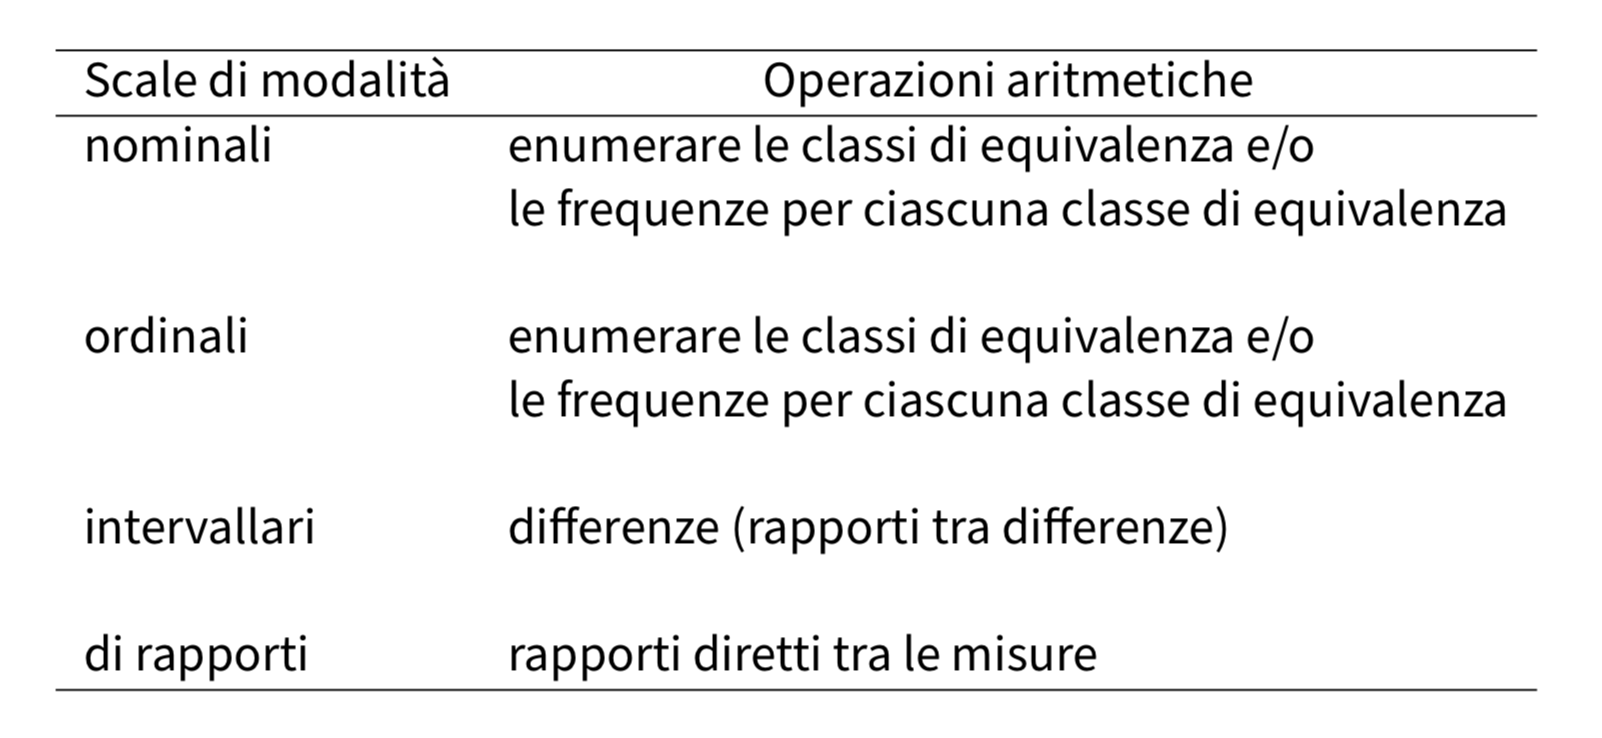
\includegraphics[width=0.8\textwidth,height=\textheight]{images/misurazione_2.png}

\hypertarget{scala-nominale}{%
\subsection{Scala nominale}\label{scala-nominale}}

Il livello di misurazione più semplice è quello della scala nominale. Questa scala di misurazione corrisponde ad una tassonomia. I simoboli o numeri che costituiscono questa scala non sono altro che i nomi delle categorie che utilizziamo per classificare i fenomeni psicologici. In base alle misure fornite da una scala nominale, l'unica cosa che siamo in grado di dire a proposito di una caratteristica psicologica è se essa è uguale o no ad un'altra caratteristica psicologica.

La scala nominale raggruppa dunque i dati in categorie qualitative \emph{mutuamente esclusive} (cioè nessun dato si può collocare in più di una categoria). Esiste la sola relazione di equivalenza tra le misure delle u.s., cioè nella scala nominale gli elementi del campione appartenenti a classi diverse sono differenti, mentre tutti quelli della stessa classe sono tra loro equivalenti: \(x_i = x_j\) oppure \(x_i \neq x_j\).

L'unica operazione algebrica che possiamo compiere sulle modalità della scala nominale è quella di contare le u.s. che appartengono ad ogni modalità e contare il numero delle modalità (classi di equivalenza). Dunque la descrizione dei dati avviene tramite le frequenze assolute e le frequenze relative.

A partire da una scala nominale è possibile costruire altre scale nominali che sono equivalenti alla prima trasformando i valori della scala di partenza in modo tale da cambiare i nomi delle modalità, ma lasciando però inalterata la suddivisione u.s. nelle medesime classi di equivalenza. Questo significa che prendendo una variabile misurata su scala nominale e cambiando i nomi delle sue categorie otteniamo una nuova variabile esattamente corrispondente alla prima.

\hypertarget{scala-ordinale}{%
\subsection{Scala ordinale}\label{scala-ordinale}}

La scala ordinale conserva la proprietà della scala nominale di classificare ciascuna u.s. all'interno di una e una sola categoria, ma alla relazione di equivalenza tra elementi di una stessa classe aggiunge la relazione di ordinamento tra le classi di equivalenza. Essendo basata su una relazione d'ordine, una scala ordinale descrive soltanto l'ordine di rango tra le modalità, ma non ci dà alcuna informazione su quanto una modalità sia più grande di un'altra. Non ci dice, per esempio, se la distanza tra le modalità \(a\) e \(b\) sia uguale, maggiore o minore della distanza tra le modalità \(b\) e \(c\).

\begin{example}
Un esempio classico di scala ordinale è quello della scala Mohs per la determinazione della durezza dei minerali. Per stabilire la durezza dei minerali si usa il criterio empirico della scalfittura. Vengono stabiliti livelli di durezza crescente da 1 a 10 con riferimento a dieci minerali: talco, gesso, calcite, fluorite, apatite, ortoclasio, quarzo, topazio, corindone e diamante. Un minerale appartenente ad uno di questi livelli se scalfisce quello di livello inferiore ed è scalfito da quello di livello superiore.
\end{example}

\hypertarget{scala-ad-intervalli}{%
\subsection{Scala ad intervalli}\label{scala-ad-intervalli}}

La scala ad intervalli include le proprietà di quella nominale e di quella ordinale, e in più consente di misurare le distanze tra le coppie di u.s. nei termini di un intervallo costante, chiamato \emph{unità di misura}, a cui viene attribuito il valore ``1''. La posizione dell'origine della scala, cioè il punto zero, è scelta arbitrariamente, nel senso che non indica l'assenza della quantità che si sta misurando. Avendo uno zero arbitrario, questa scala di misura consente valori negativi. Lo zero, infatti, \emph{non} viene attribuito all'u.s. in cui la proprietà misurata risulta assente.

La scala a intervalli equivalenti ci consente di effettuare operazioni algebriche basate sulla differenza tra i numeri associati ai diversi punti della scala, operazioni algebriche non era possibile eseguire nel caso di misure a livello di scala ordinale o nominale. Il limite della scala ad intervalli è quello di non consentire il calcolo del rapporto tra coppie di misure. Possiamo dire, per esempio, che la distanza tra \(a\) e \(b\) è la metà della distanza tra \(c\) e \(d\). Oppure che la distanza tra \(a\) e \(b\) è uguale alla distanza tra \(c\) e \(d\). Non possiamo dire, però, che \(a\) possiede la proprietà misurata in quantità doppia rispetto \(b\). Non possiamo cioè stabilire dei rapporti diretti tra le misure ottenute. Solo per le \emph{differenze} tra le modalità sono dunque permesse tutte le operazioni aritmetiche: le differenze possono essere tra loro sommate, elevate a potenza oppure divise, determinando così le quantità che stanno alla base della statistica inferenziale.

Nelle scale ad intervalli equivalenti, l'unità di misura è arbitraria, ovvero può essere cambiata attraverso una dilatazione, operazione che consiste nel moltiplicare tutti i valori della scala per una costante positiva. Poiché l'aggiunta di una costante non altera le differenze tra i valori della scala, è anche ammessa la traslazione, operazione che consiste nel sommare una costante a tutti i valori della scala. Essendo la scala invariate rispetto alla traslazione e alla dilatazione, le trasformazioni ammissibili sono le \emph{trasformazioni lineari}:

\[
y' = a + by, \quad b > 0.
\] L'aspetto che rimane invariante a seguito di una trasformazione lineare è l'uguaglianza dei rapporti fra intervalli.

\begin{example}
Esempio di scala ad intervalli è la temperatura misurata in gradi Celsius o Fahrenheit, ma non Kelvin. Come per la scala nominale, è possibile stabilire se due modalità sono uguali o diverse: 30\(^\circ\)C \(\neq\) 20\(^\circ\)C. Come per la scala ordinale è possibile mettere due modalità in una relazione d'ordine: 30\(^\circ\)C \(>\) 20\(^\circ\)C. In aggiunta ai casi precedenti, però, è possibile definire una unità di misura per cui è possibile dire che tra 30\(^\circ\)C e 20\(^\circ\)C c'è una differenza di 30\(^\circ\) - 20\(^\circ\) = 10\(^\circ\)C. I valori di temperatura, oltre a poter essere ordinati secondo l'intensità del fenomeno, godono della proprietà che le differenze tra loro sono direttamente confrontabili e quantificabili.

Il limite della scala ad intervalli è quello di non consentire il calcolo del rapporto tra coppie di misure. Ad esempio, una temperatura di 80\(^\circ\)C non è il doppio di una di 40\(^\circ\)C. Se infatti esprimiamo le stesse temperature nei termini della scala Fahrenheit, allora i due valori non saranno in rapporto di 1 a 2 tra loro. Infatti, 20\(^\circ\)C = 68\(^\circ\)F e 40\(^\circ\)C = 104\(^\circ\)F. Questo significa che la relazione ``il doppio di'' che avevamo individuato in precedenza si applicava ai numeri della scala centigrada, ma non alla proprietà misurata (cioè la temperatura). La decisione di che scala usare (Centigrada vs.~Fahrenheit) è arbitraria. Ma questa arbitrarietà non deve influenzare le inferenze che traiamo dai dati. Queste inferenze, infatti, devono dirci qualcosa a proposito della realtà empirica e non possono in nessun modo essere condizionate dalle nostre scelte arbitrarie che ci portano a scegliere la scala Centigrada piuttosto che quella Fahrenheit.

Consideriamo ora l'aspetto invariante di una trasformazione lineare, ovvero l'uguaglianza dei rapporti fra intervalli. Prendiamo in esame, ad esempio, tre temperature: \(20^\circ C = 68^\circ F\), \(15^\circ C = 59^\circ F\), \(10^\circ C = 50 ^\circ F\).

È facile rendersi conto del fatto che i rapporti fra intervalli restano costanti indipendentemente dall'unità di misura che è stata scelta:

\[
  \frac{20^\circ C - 10^\circ C}{20^\circ C - 15^\circ C} =
  \frac{68^\circ F - 50^\circ F}{68^\circ F-59^\circ F} = 2.
\]
\end{example}

\hypertarget{scala-di-rapporti}{%
\subsection{Scala di rapporti}\label{scala-di-rapporti}}

Nella scala a rapporti equivalenti la posizione dello zero non è arbitraria, ma corrisponde all'elemento dotato di intensità nulla rispetto alla proprietà misurata. Una scala a rapporti equivalenti si costruisce associando il numero 0 all'elemento con intensità nulla; viene poi scelta un'unità di misura \(u\) e, ad ogni elemento, si assegna un numero \(a\) definito come: \[a = \frac{d}{u}\] dove \(d\) rappresenta la distanza dall'origine. Alle u.s. vengono dunque assegnati dei numeri tali per cui le differenze e i rapporti tra i numeri riflettono le differenze e i rapporti tra le intensità della proprietà misurata.

Operazioni aritmetiche sono possibili non solo sulle differenze tra i valori della scala (come per la scala a intervalli equivalenti), ma anche sui valori stessi della scala. L'unica arbitrarietà riguarda l'unità di misura che si utilizza. L'unità di misura può cambiare, ma qualsiasi unità di misura si scelga, lo zero deve sempre indicare l'intensità nulla della proprietà considerata.

Le trasformazioni ammissibili a questo livello di scala sono dette trasformazioni di similarità: \[y' = by, \quad b > 0.\] A questo livello di scala, a seguito delle trasformazioni ammissibili, rimangono invariati anche i rapporti: \[\frac{y_i}{y_j} = \frac{y'_i}{y'_j}.\]

\hypertarget{gerarchia-dei-livelli-di-scala-di-misura}{%
\section{Gerarchia dei livelli di scala di misura}\label{gerarchia-dei-livelli-di-scala-di-misura}}

\citet{stevens46} parla di \emph{livelli di scala} poiché i quattro tipi di scala di misura stanno in una precisa gerarchia: la scala nominale rappresenta il livello più basso della misurazione, la scala a rapporti equivalenti è invece il livello più alto.

\begin{longtable}[]{@{}
  >{\raggedright\arraybackslash}p{(\columnwidth - 2\tabcolsep) * \real{0.2576}}
  >{\raggedright\arraybackslash}p{(\columnwidth - 2\tabcolsep) * \real{0.7424}}@{}}
\toprule
\begin{minipage}[b]{\linewidth}\raggedright
Scale di modalità
\end{minipage} & \begin{minipage}[b]{\linewidth}\raggedright
Operazioni aritmetiche
\end{minipage} \\
\midrule
\endhead
nominali & enumerare le classi di equivalenza e/o \\
& le frequenze per ciascuna classe di equivalenza \\
ordinali & enumerare le classi di equivalenza e/o \\
& le frequenze per ciascuna classe di equivalenza \\
intervallari & differenze (rapporti tra differenze) \\
di rapporti & rapporti diretti tra le misure \\
\bottomrule
\end{longtable}

Passando da un livello di misurazione ad uno più alto aumenta il numero di operazioni aritmetiche che possono essere compiute sui valori della scala, come indicato nella figura seguente.

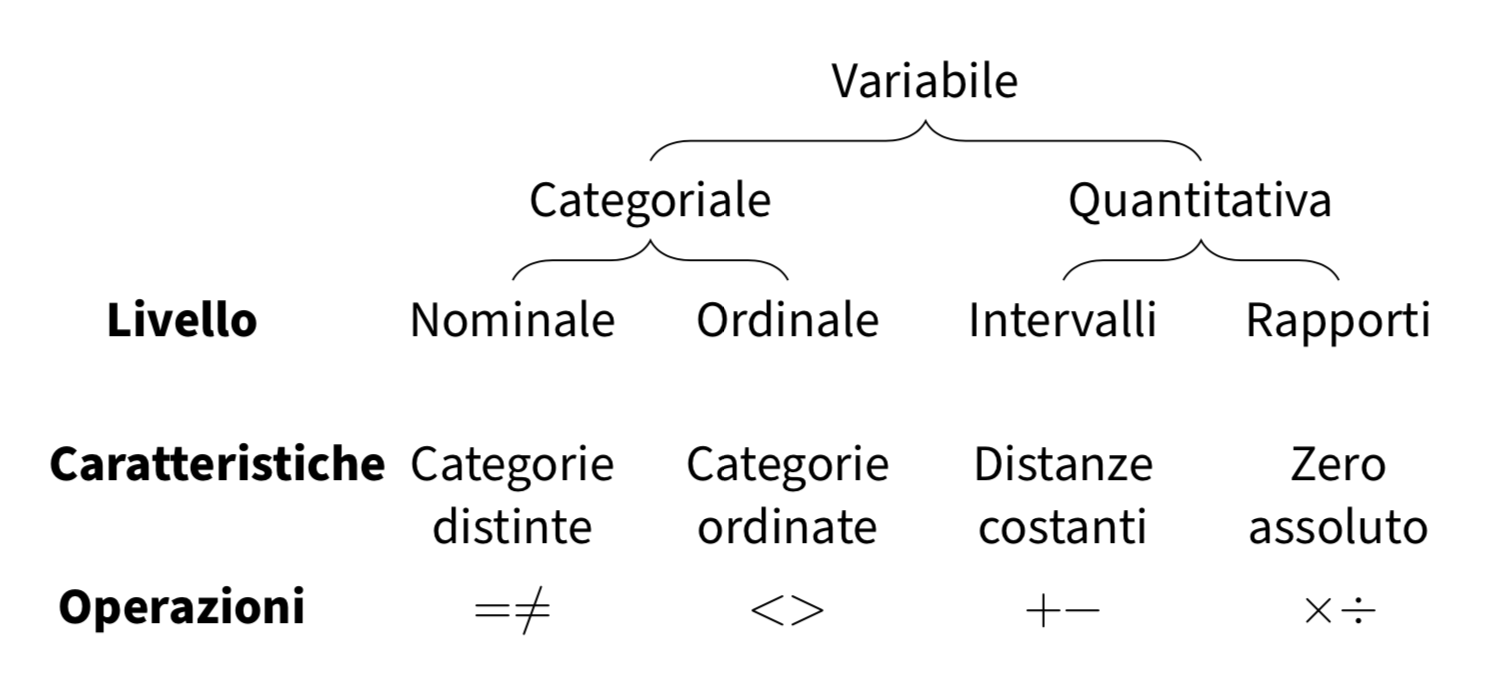
\includegraphics[width=0.8\textwidth,height=\textheight]{images/misurazione_1.png}

Per ciò che riguarda le trasformazioni ammissibili, più il livello di scala è basso, più le funzioni sono generali (sono minori cioè i vincoli per passare da una rappresentazione numerica ad un'altra equivalente). Salendo la gerarchia, la natura delle funzioni di trasformazione si fa più restrittiva.

\hypertarget{variabili-discrete-o-continue}{%
\section{Variabili discrete o continue}\label{variabili-discrete-o-continue}}

Le variabili a livello di intervalli e di rapporti possono essere discrete o continue. Le variabili discrete possono assumere alcuni valori ma non altri. Una volta che l'elenco di valori accettabili è stato specificato, non ci sono casi che cadono tra questi valori. Le variabili discrete di solito assumono valori interi.

Quando una variabile può assumere qualsiasi valore entro un intervallo specificato, allora si dice che la variabile è continua. In teoria, ciò significa che frazioni e decimali possono essere utilizzati per raggiungere un livello di precisione qualsiasi. In pratica, a un certo punto dobbiamo arrotondare i numeri, rendendo tecnicamente la variabile discreta. In variabili veramente discrete, tuttavia, non è possibile aumentare a piacimento il livello di precisione della misurazione.

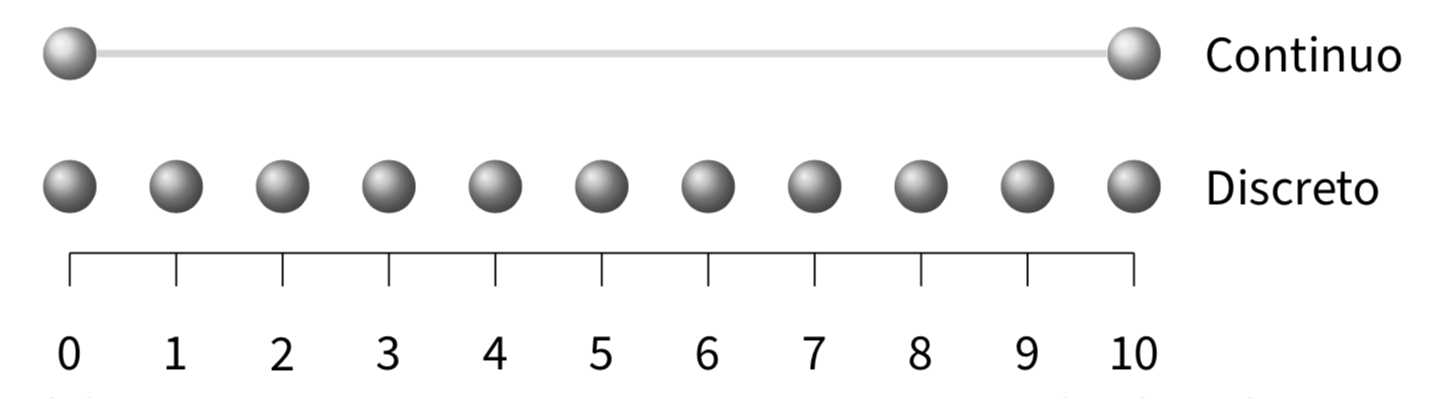
\includegraphics[width=0.8\textwidth,height=\textheight]{images/misurazione_3.png}

\begin{example}
Il numero di biciclette possedute da una persona è una variabile discreta poiché tale variabile può assumere come modalità solo i numeri interi non negativi. Frazioni di bicicletta non hanno senso.
\end{example}

\hypertarget{alcune-misure-sono-migliori-di-altre}{%
\section{Alcune misure sono migliori di altre}\label{alcune-misure-sono-migliori-di-altre}}

In psicologia, ciò che vogliamo misurare non è una caratteristica fisica, ma invece è un concetto teorico inosservabile, ovvero un costrutto.

\begin{quote}
Un costrutto rappresenta il risultato di una fondata riflessione scientifica, non è per definizione accessibile all'osservazione diretta, ma viene inferito dall'osservazione di opportuni indicatori (Sartori, 2005).
\end{quote}

Ad esempio, supponiamo che un docente voglia valutare quanto bene uno studente comprenda la distinzione tra le quattro diverse scale di misura che sono state descritte sopra. Il docente potrebbe predisporre un test costituito da un insieme di domande e potrebbe contare a quante domande lo studente risponde correttamente. Questo test, però, può o può non essere una buona misura del costrutto relativo alla conoscenza effettiva delle quattro scale di misura. Per esempio, se il docente scrive le domande del test in modo ambiguo o se usa una linguaggio troppo tecnico che lo studente non conosce, allora i risultati del test potrebbero suggerire che lo studente non conosce la materia in questione anche se in realtà questo non è vero. D'altra parte, se il docente prepara un test a scelta multipla con risposte errate molto ovvie, allora lo studente può ottenere dei buoni risultati al test anche senza essere in grado di comprendere adeguatamente le proprietà delle quattro scale di misura.

In generale non è possibile misurare un costrutto senza una certa quantità di errore. Poniamoci dunque il problema di determinare in che modo una misurazione possa dirsi adeguata.

\hypertarget{tipologie-di-errori}{%
\subsection{Tipologie di errori}\label{tipologie-di-errori}}

L'errore è, per definizione, la differenza tra il valore vero e il valore misurato della grandezza in esame. Gli errori sono classificati come sistematici (o determinati) e casuali (o indeterminati). Gli errori casuali sono fluttuazioni, in eccesso o in difetto rispetto al valore reale, delle singole determinazioni e sono dovuti alle molte variabili incontrollabili che influenzano ogni misura psicologica. Gli errori sistematici, invece, influiscono sulla misurazione sempre nello stesso senso e, solitamente, per una stessa quantità (possono essere additivi o proporzionali).

Le differenze tra le due tipologie di errori, sistematici e casuali, introducono i concetti di accuratezza e di precisione della misura. Una misura viene definita:

\begin{itemize}
\tightlist
\item
  \emph{accurata}, quando vi è un accordo tra la misura effettuata ed il valore reale;
\item
  \emph{precisa} quando, ripetendo più volte la misura, i risultati ottenuti sono concordanti, cioè differiscono in maniera irrilevante tra loro.
\end{itemize}

La metafora del tiro a bersaglio illustra la relazione tra precisione e accuratezza.

\begin{figure}[h]

{\centering 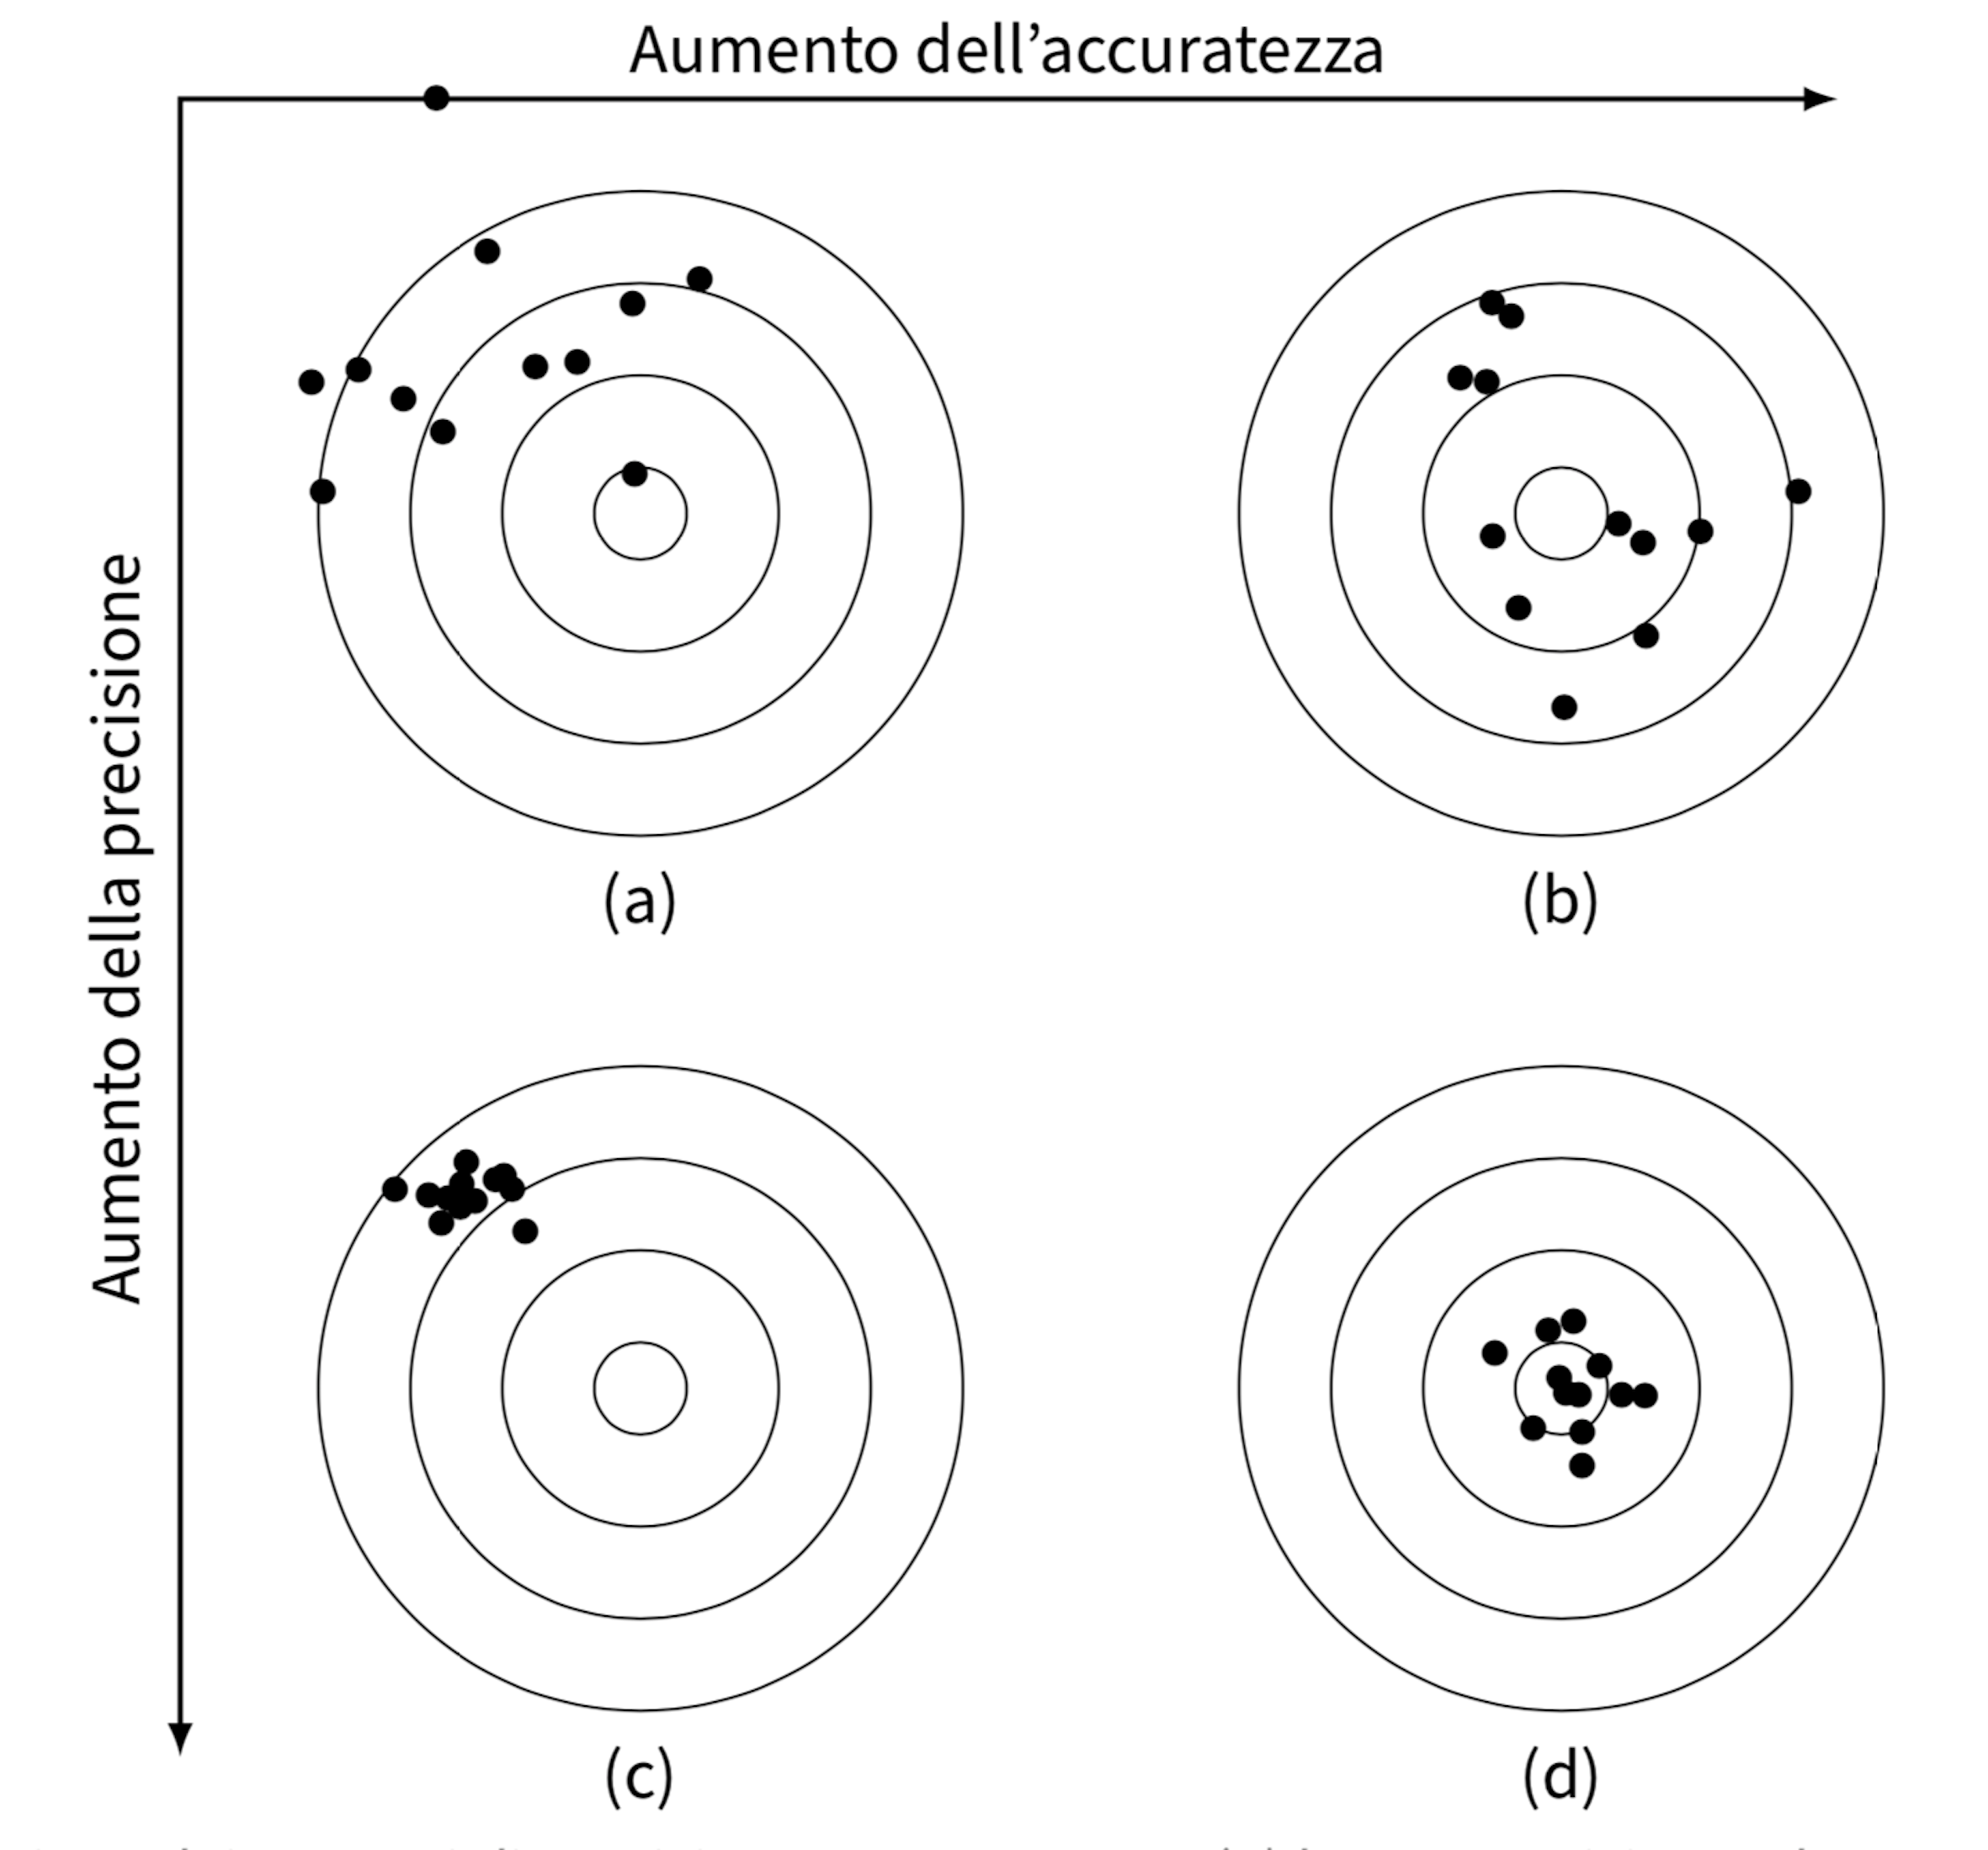
\includegraphics[width=7.87in]{images/misurazione_4} 

}

\caption{Metafora del tiro al bersaglio.}\label{fig:fig-tiro-bersaglio}
\end{figure}

Per tenere sotto controllo l'incidenza degli errori, sono stati introdotti in psicologia i concetti di attendibilità e validità.

Uno strumento si dice \emph{attendibile} quando valuta in modo coerente e stabile la stessa variabile: i risultati ottenuti si mantengono costanti dopo ripetute somministrazione ed in assenza di variazioni psicologiche e fisiche dei soggetti sottoposti al test o cambiamenti dell'ambiente in cui ha luogo la somministrazione.

L'attendibilità di uno strumento, però, non è sufficiente: in primo luogo uno strumento di misura deve essere \emph{valido}, laddove la validità rappresenta il grado in cui uno strumento misura effettivamente ciò che dovrebbe misurare. In genere, si fa riferimento ad almeno quattro tipi di validità.

\begin{itemize}
\tightlist
\item
  La \emph{validità di costrutto} riguarda il grado in cui un test misura ciò per cui è stato costruito. Essa si suddivide in: validità convergente e validità divergente. La validità convergente fa riferimento alla concordanza tra uno strumento e un altro che misura lo stesso costrutto. La validità divergente, al contrario, valuta il grado di discriminazione tra strumenti che misurano costrutti differenti. Senza validità di costrutto le altre forme di validità non hanno senso.
\item
  In base alla \emph{validità di contenuto}, un test fornisce una misura valida di un attributo psicologico se il dominio dell'attributo è rappresentato in maniera adeguata dagli item del test. Un requisito di base della validità di contenuto è la rilevanza e la rappresentatività del contenuto degli item in riferimento all'attributo che il test intende misurare.
\item
  La \emph{validità di criterio} valuta il grado di concordanza tra i risultati dello strumento considerato e i risultati ottenuti da altri strumenti che misurano lo stesso costrutto, o tra i risultati dello strumento considerato e un criterio esterno. Nella validità concorrente, costrutto e criterio vengono misurati contestualmente, consentendo un confronto immediato. Nella validità predittiva, il costrutto viene misurato prima e il criterio in un momento successivo, consentendo la valutazione della capacità dello strumento di predire un evento futuro.
\item
  Infine, la \emph{validità di facciata} fa riferimento al grado in cui il test appare valido ai soggetti a cui esso è diretto. La validità di facciata è importante in ambiti particolari, quali ad esempio la selezione del personale per una determinata occupazione. In questo caso è ovviamente importante che chi si sottopone al test ritenga che il test vada a misurare quegli aspetti che sono importanti per le mansioni lavorative che dovranno essere svolte, piuttosto che altre cose. In generale, la validità di facciata non è utile, tranne in casi particolari.
\end{itemize}

\hypertarget{conclusioni}{%
\section*{Conclusioni}\label{conclusioni}}


Una domanda che uno psicologo spesso si pone è: ``sulla base delle evidenze osservate, possiamo concludere dicendo che l'intervento psicologico è efficace nel trattamento e nella cura del disturbo?'' Le considerazioni svolte in questo capitolo dovrebbero farci capire che, prima di cercare di rispondere a questa domanda con l'analisi statistica dei dati, devono essere affrontati i problemi della validità e dell'attendibilità delle misure (oltre a stabilire l'appropriato livello di scala di misura delle osservazioni). L'attendibilità è un prerequisito della validità. Se gli errori di misurazione sono troppo grandi, i dati sono inutili. Inoltre, uno strumento di misurazione può essere preciso ma non valido. La validità e l'attendibilità delle misurazioni sono dunque entrambe necessarie.

In generale, l'attendibilità e la validità delle misure devono essere valutate per capire se i dati raccolti da un ricercatore siano adeguati (1) per fornire una risposta alla domanda della ricerca, e (2) per giungere alla conclusione proposta dal ricercatore alla luce dei risultati dell'analisi statistica che è stata eseguita. È chiaro che le informazioni fornite in questo capitolo si limitano a scalfire la superficie di questi problemi. I concetti qui introdotti, però, devono sempre essere tenuti a mente e costituiscono il fondamento di quanto verrà esposto nei capitoli successivi.

\mainmatter

\hypertarget{part-nozioni-di-base}{%
\part*{Nozioni di base}\label{part-nozioni-di-base}}


\hypertarget{intro-prob-1}{%
\chapter{Il calcolo delle probabilità}\label{intro-prob-1}}

Una possibile definizione di teoria delle probabilità è la seguente: la teoria delle probabilità ci fornisce gli strumenti per prendere decisioni razionali in condizioni di incertezza, ovvero per formulare le migliori congetture possibili.

\hypertarget{inf-stat-probl-inv}{%
\section{La probabilità come la logica della scienza}\label{inf-stat-probl-inv}}

La figura \ref{fig:cycle-of-science} fornisce una rappresentazione schematica del processo dell'indagine scientifica. Possiamo pensare al progresso scientifico come alla ripetizione di questo ciclo, laddove i fenomeni naturali (e, ovviamente psicologici) vengono esplorati e i ricercatori imparano sempre di più sul loro funzionamento. Le caselle della figura descrivono le varie fasi del processo di ingagine scientifica, mentre lungo le frecce sono riportati i compiti che conducono i ricercatori da una fase alla successiva.

\begin{figure}[h]

{\centering 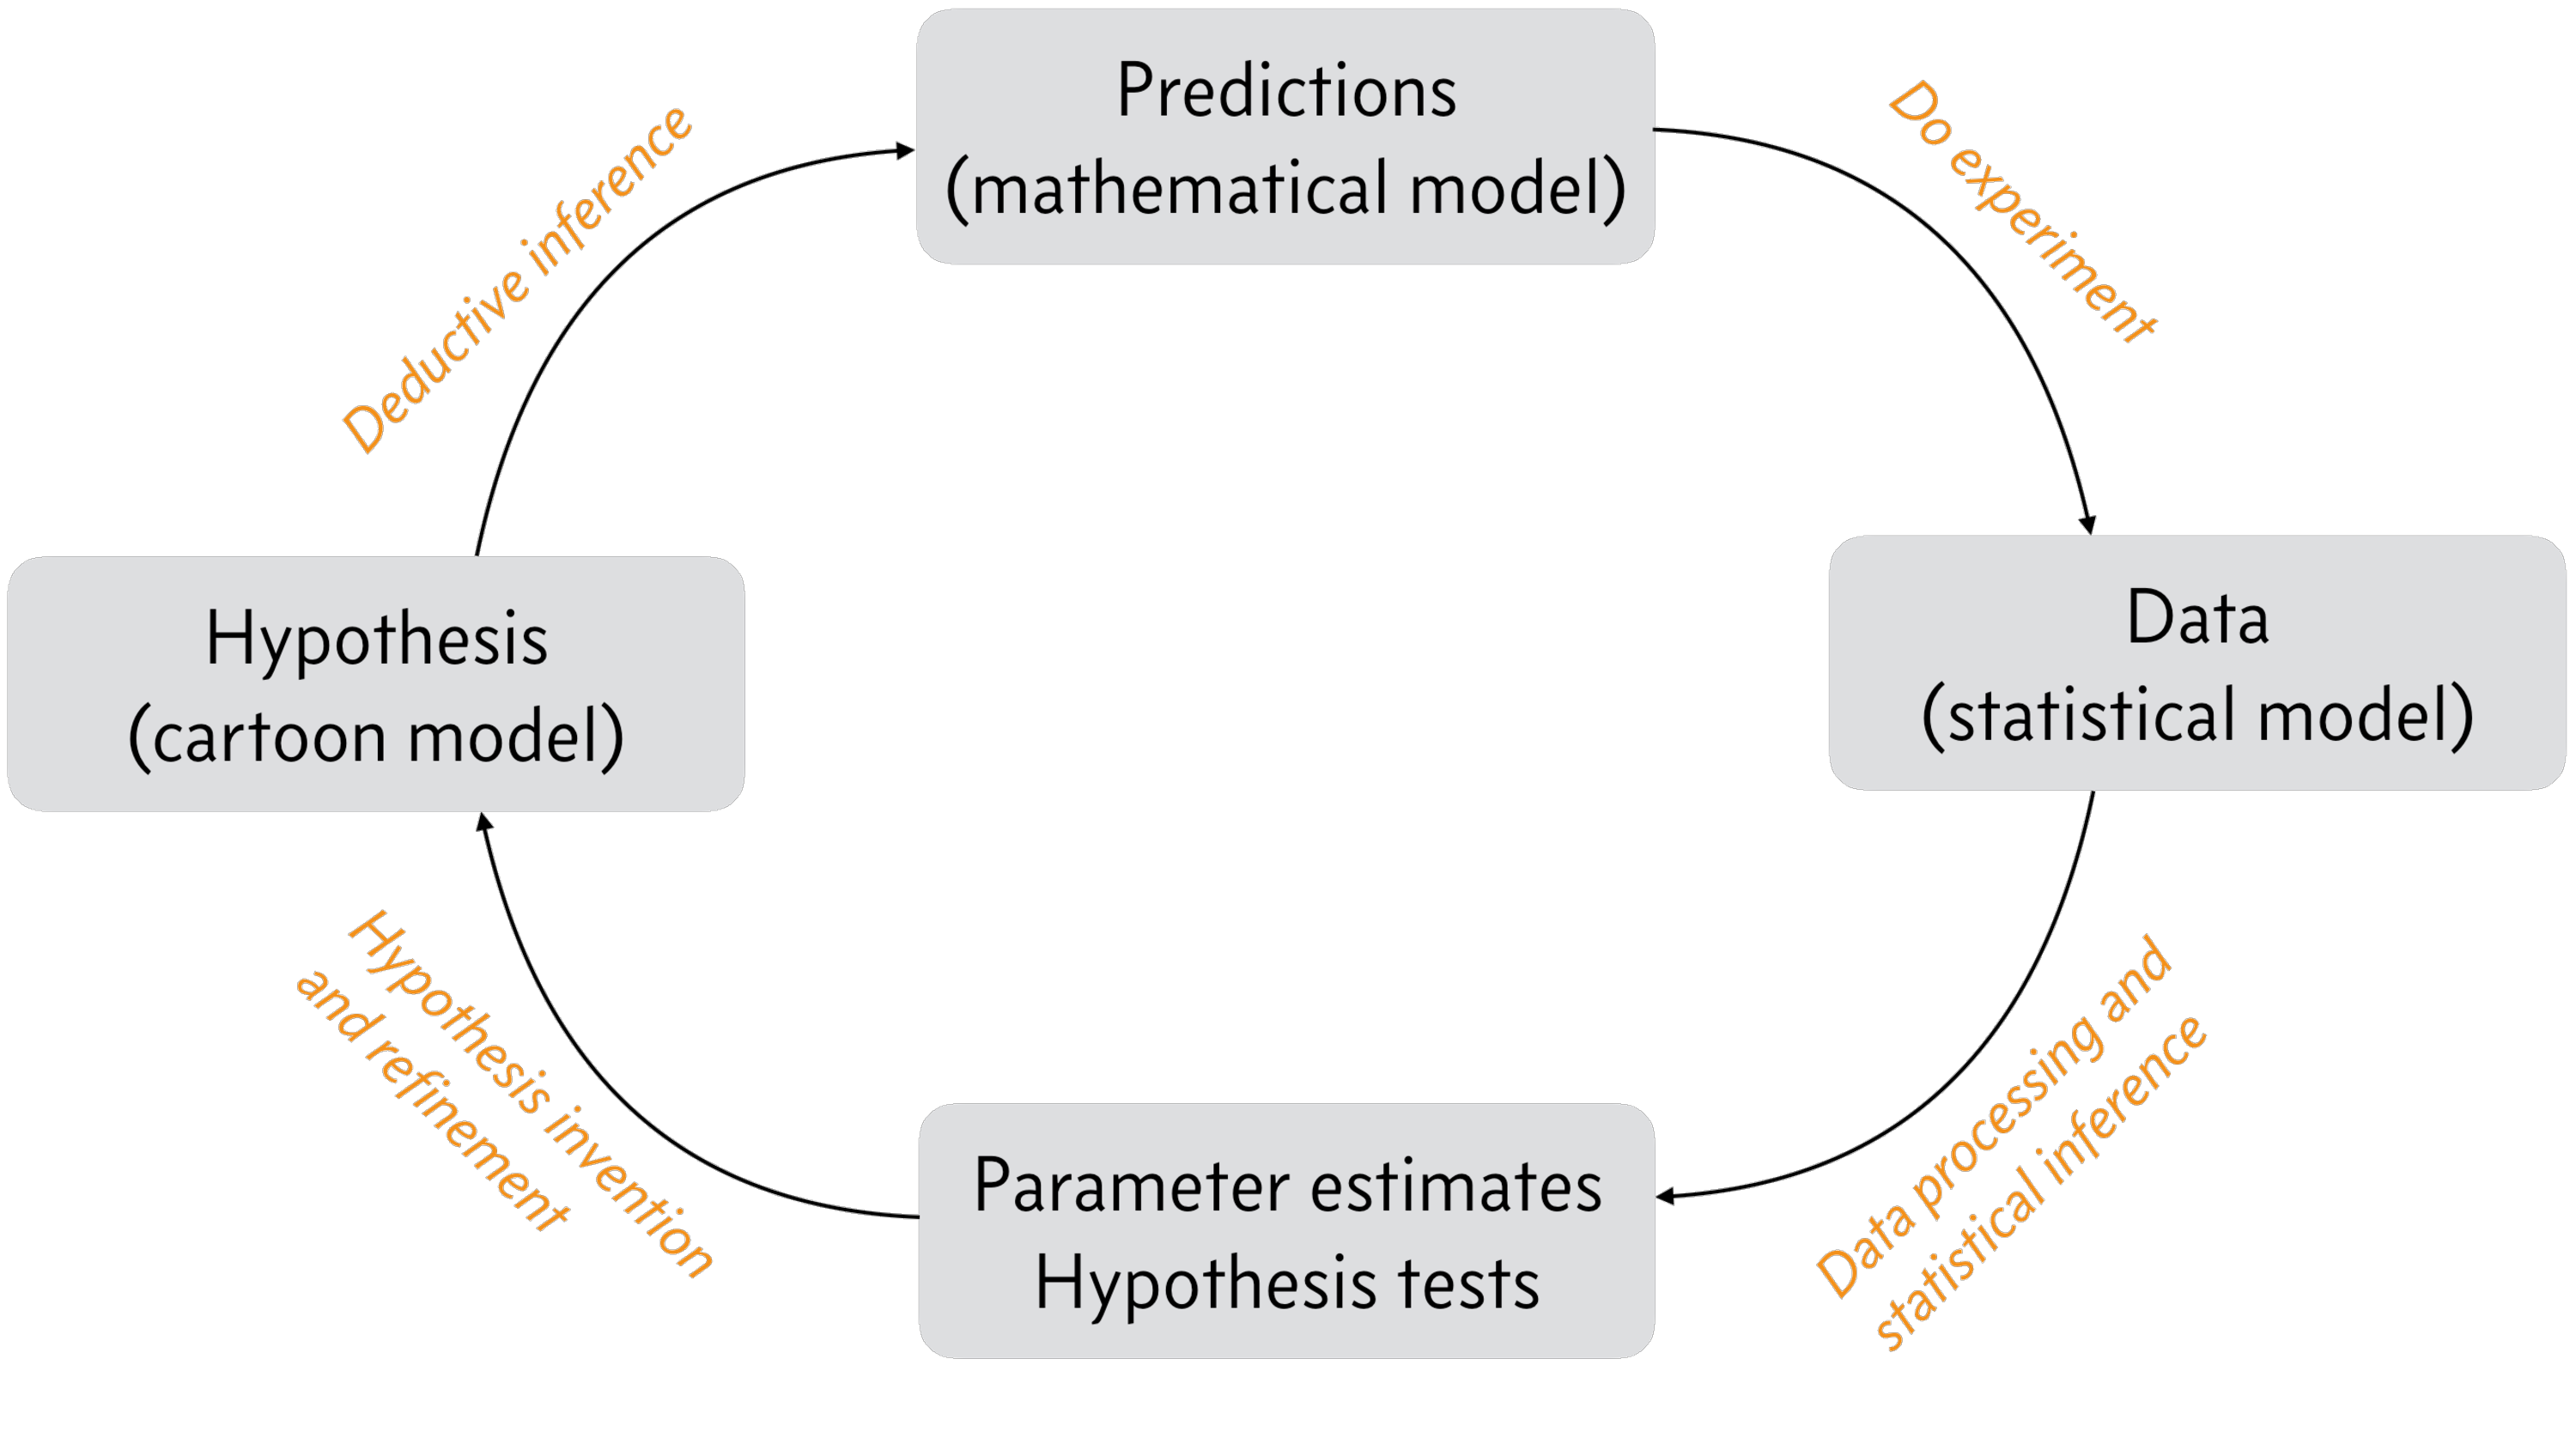
\includegraphics{images/cycle_of_science} 

}

\caption{Rappresentazione schematica del processo scientifico (figura adattata dalla Fig. 1.1 di P. Gregory, Bayesian Logical Data Analysis for the Physical Sciences, Cambridge, 2005).}\label{fig:cycle-of-science}
\end{figure}

Consideriamo i compiti e le fasi dell'indagine scientifica. Iniziamo in basso a sinistra.

\begin{itemize}
\item
  \emph{Invenzione e perfezionamento delle ipotesi.} In questa fase del processo scientifico, i ricercatori pensano ai fenomeni naturali, a ciò che è presente nella letteratura scientifica, ai risultati dei loro esperimenti, e formulano ipotesi o teorie che possono essere valutare mediante esperimenti empirici. Questo passaggio richiede innovazione e creatività.
\item
  L'\emph{inferenza deduttiva} procede in maniera deterministica dai fatti alle conclusioni. Ad esempio, se dico che tutti gli uomini sono mortali e che Socrate è un uomo, allora posso concludere deduttivamente che Socrate è mortale. Quando i ricercatori progettano gli esperimenti in base alle teorie, usano la logica deduttiva per dire: ``Se A è vero, allora B deve essere vero'', dove \(A\) è l'ipotesi teorica e \(B\) è l'osservazione sperimentale.
\item
  \emph{Esecuzione degli esperimenti.} Questa fase richiede molte risorse (tempo e denaro). Richiede anche innovazione e creatività. Nello specifico, i ricercatori devono pensare attentamente a come costruire l'esperimento necessario per verificare la teoria di interesse. Quale risultato dell'esperimento si ottengono i dati.
\item
  L'\emph{inferenza induttiva} procede dalle osservazioni ai fatti. Se pensiamo ai fatti come a ciò che governa o genera le osservazioni, allora l'induzione è una sorta di inferenza inversa. Supponiamo di avere osservato \(B\). Questo rende \(A\) vero? Non necessariamente. Ma può rendere \(A\) più plausibile. Questo è un sillogismo debole. Ad esempio, si consideri la seguente coppia ipotesi/osservazioni.

  \begin{itemize}
  \item
    \(A\) = L'iniezione di acque reflue dopo la fratturazione idraulica, nota come fracking, può portare a una maggiore frequenza di terremoti.
  \item
    \(B\) = La frequenza dei terremoti in Oklahoma è aumentata di 100 volte dal 2010, quando il fracking è diventato una pratica comune.
  \item
    Poiché \(B\) è stato osservato, \(A\) è più plausibile. \(A\) non è necessariamente vero, ma è più plausibile.
  \end{itemize}
\item
  L'\emph{inferenza statistica} è un tipo di inferenza induttiva che è specificamente formulata come un problema inverso. L'inferenza statistica è quell'insieme di procedure che hanno lo scopo di quantificare quanto più plausibile sia \(A\) dopo aver osservato \(B\). Per svolgere l'inferenza statistica è dunque necessario quantificare tale plausibilità. Lo strumento che ci consente di fare questo è la teoria delle probabilità.
\end{itemize}

L'inferenza statistica è l'aspetto del processo dell'indagine scientifica che è l'oggetto centrale di questo insegnamento. Il risultato dell'inferenza statistica è la conoscenza di quanto siano plausibili le ipotesi e le stime dei parametri sotto le ipotesi considerate. Ma l'inferenza statistica richiede una teoria delle probabilità, laddove la teoria delle probabilità può essere vista come una generalizzazione della logica. A causa di questa connessione con la logica e del suo ruolo cruciale nella scienza, E. T. Jaynes afferma infatti che la probabilità è la ``logica della scienza''. È dunque necessario esaminare preliminarmente alcune nozioni di base della teoria delle probabilità.

\hypertarget{che-cosuxe8-la-probabilituxe0}{%
\section{Che cos'è la probabilità?}\label{che-cosuxe8-la-probabilituxe0}}

La definizione della probabilità è un problema estremamente dibattuto ed aperto. Sono state fornite due possibili soluzioni al problema di definire il concetto di probabilità.

\begin{enumerate}
\def\labelenumi{(\alph{enumi})}
\item
  La natura della probabilità è ``ontologica'' (ovvero, basata sulla metafisica): la probabilità è una proprietà della della realtà, del mondo, di come sono le cose, indipendentemente dalla nostra esperienza. È una visione che qualcuno chiama ``oggettiva''.
\item
  La natura della probabilità è ``epistemica'' (ovvero, basata sulla conoscenza): la probabilità si riferisce alla conoscenza che abbiamo del mondo, non al mondo in sé. Di conseguenza è detta, in contrapposizione alla precedente definizione, ``soggettiva''.
\end{enumerate}

In termini epistemici, la probabilità fornisce una misura della nostra incertezza sul verificarsi di un fenomeno, alla luce delle informazioni disponibili. Potremmo dire che c'è una ``scala'' naturale che ha per estremi il vero (1: evento certo) da una parte ed il falso (0: evento impossibile) dall'altra. La probabilità è la quantificazione di questa scala: quantifica lo stato della nostra incertezza rispetto al contenuto di verità di una proposizione (ovvero, quantifica la plausibilità di una proposizione).

\begin{itemize}
\item
  Nell'interpretazione frequentista della probabilità, la probabilità \(P(A)\) rappresenta la frequenza relativa a lungo termine nel caso di un grande numero di ripetizioni di un esperimento casuale sotto le medesime condizioni. L'evento \(A\) deve essere una proposizione relativa alle variabili casuali\footnote{Viene stressata qui l'idea che ciò di cui parliamo è qualcosa che emerge nel momento in cui è possibile ripetere l'esperimento casuale tante volte sotto le medesime condizioni. Le variabili casuali, infatti, forniscono una quantificazione dei risultati che si ottengono ripetendo tante volte l'esperimento casuale sotto le medesime condizioni.}.
\item
  Nell'interpretazione bayesiana della probabilità \(P(A)\) rappresenta il grado di credenza, o plausibilità, a proposito di \(A\), dove \(A\) può essere qualsiasi proposizione logica.
\end{itemize}

In questo insegnamento utilizzeremo l'interpretazione bayesiana della probabilità. Possiamo citare De Finetti, ad esempio, il quale ha formulato la seguente definizione ``soggettiva'' di probabilità la quale risulta applicabile anche ad esperimenti casuali i cui eventi elementari non siano ritenuti ugualmente possibili e che non siano necessariamente ripetibili più volte sotto le stesse condizioni:

\begin{definition}
La probabilità di un evento \(E\) è la quota \(p(E)\) che un individuo reputa di dover pagare ad un banco per ricevere ``1'' ovvero ``0'' verificandosi o non verificandosi \(E\). Le valutazioni di probabilità degli eventi devono rispondere ai pricipi di equità e coerenza.
\end{definition}

I principi di equità e coerenza sono definiti come segue.

\begin{definition}
Una scommessa risponde ai pricipi di \emph{equità} se il ruolo di banco e giocatore sono scambiabili in ogni momento del gioco e sempre alle stesse condizioni; \emph{coerenza} se non vi sono combinazioni di scommesse che consentano (sia al banco che al giocatore) di realizzare perdite o vincite certe.
\end{definition}

Secondo \citet{definetti1931prob}, \emph{nessuna scienza ci permetterà di dire: il tale fatto accadrà, andrà così e così, perché ciò è conseguenza di tale legge, e tale legge è una verità assoluta, ma tanto meno ci condurrà a concludere scetticamente: la verità assoluta non esiste, e quindi tale fatto può accadere e può non accadere, può andare così e può andare in tutt'altro modo, nulla io ne so. Quel che si potrà dire è questo: io prevedo che il tale fatto avverrà, e avverrà nel tal modo, perché l'esperienza del passato e l'elaborazione scientifica cui il pensiero dell'uomo l'ha sottoposta mi fanno sembrare ragionevole questa previsione.}

In altri termini, de Finetti ritiene che la probabilità debba essere concepita non come una proprietà ``oggettiva'' dei fenomeni (``la probabilità di un fenomeno ha un valore determinato che dobbiamo solo scoprire''), ma bensì come il ``grado di fiducia -- in inglese \emph{degree of belief} -- di un dato soggetto, in un dato istante e con un dato insieme d'informazioni, riguardo al verificarsi di un evento''. Per denotare sia la probabilità (soggettiva) di un evento sia il concetto di \emph{valore atteso} (che descriveremo in seguito), \citet{definetti1970teoria} utilizza il termine ``previsione'' (e lo stesso simbolo \(P\)): \emph{la previsione {[}\(\dots\){]} consiste nel considerare ponderatamente tutte le alternative possibili per ripartire fra di esse nel modo che parrà più appropriato le proprie aspettative, le proprie sensazioni di probabilità.}

\hypertarget{variabili-casuali-e-probabilituxe0-di-un-evento}{%
\section{Variabili casuali e probabilità di un evento}\label{variabili-casuali-e-probabilituxe0-di-un-evento}}

Esaminiamo qui di seguito alcuni concetti di base della teoria delle probabilità.

\hypertarget{variabili-casuali-1}{%
\subsection{Variabili casuali}\label{variabili-casuali-1}}

Sia \(Y\) il risultato del lancio di moneta equilibrata, non di un generico lancio di una moneta, ma un'istanza specifica del lancio di una specifica moneta in un dato momento. Definita in questo modo, \(Y\) è una \emph{variabile casuale}, ovvero una variabile che assume valori diversi con probabilità diverse. Se la moneta è equilibrata, c'è una probabilità del 50\% che il lancio della moneta dia come risultato ``testa'' e una probabilità del 50\% che dia come risultato ``croce''.

Per facilitare la trattazione, le variabili casuali assumono solo valori numerici. Per lo specifico lancio della moneta in questione, diciamo, ad esempio, che la variabile casuale \(Y\) assume il valore 1 se esce testa e il valore 0 se esce croce.

\hypertarget{eventi-e-probabilituxe0}{%
\subsection{Eventi e probabilità}\label{eventi-e-probabilituxe0}}

Nella teoria delle probabilità il risultato ``testa'' nel lancio di una moneta è chiamato \emph{evento}.\footnote{Per un ripasso delle nozioni di base della teoria degli insiemi, si veda l'Appendice \ref{insiemistica}.} Ad esempio, \(Y\) = 1 denota l'evento in cui il lancio di una moneta produce come risultato testa.

Il funzionale \(Pr[·]\) definisce la probabilità di un evento. Ad esempio, per il lancio di una moneta equilibrata, la probabilità dell'evento ``il risultato del lancio della moneta è testa'' è scritta come

\[
Pr[Y = 1] = 0.5.
\] Se la moneta è equilibrata dobbiamo anche avere \(Pr[Y = 0] = 0.5\). I due eventi \emph{Y} = 1 e \(Y\) = 0 sono \emph{mutuamente esclusivi} nel senso che non possono entrambi verificarsi contemporaneamente. Nella notazione probabilistica,

\[
Pr[Y = 1\; e \; Y = 0] = 0.
\] Gli eventi \(Y\) = 1 e \(Y\) = 0 di dicono \emph{esaustivi}, nel senso che almeno uno di essi deve verificarsi e nessun altro tipo di evento è possibile. Nella notazione probabilistica,

\[
Pr[Y = 1\; o \; Y = 0] = 1.
\] Il connettivo logico ``e'' specifica eventi \emph{congiunti}, ovvero eventi che possono verificarsi contemporaneamente (eventi \emph{compatibili}) e per i quali, perciò, la probabilità della loro congiunzione è \(Pr(A \; e \; B) > 0\). Il connettivo logico ``o'' specifica eventi \emph{disgiunti}, ovvero eventi che non possono verificarsi contemporaneamente (eventi \emph{incompatibili}) e per i quali, perciò, la probabilità della loro congiunzione è \(P(A \; e \; B) = 0\).

\hypertarget{spazio-campionario-e-risultati-possibili}{%
\section{Spazio campionario e risultati possibili}\label{spazio-campionario-e-risultati-possibili}}

Anche se il lancio di una moneta produce sempre uno specifico risultato nel mondo reale, noi possiamo anche immaginare i possibili risultati alternativi che si sarebbero potuti osservare. Quindi, anche se in uno specifico lancio la moneta dà testa (\(Y\) = 1), possiamo immaginare la possibilità che il lancio possa avere prodotto croce (\(Y\) = 0). Tale ragionamento controfattuale è la chiave per comprendere la teoria delle probabilità e l'inferenza statistica.

I risultati possibili che si possono osservare come conseguenza del lancio di una moneta determinano i valori possibili che la variabile casuale può assumere. L'insieme di tutti i risultati possibili è chiamato \emph{spazio campionario}. Lo spazio campionario può essere concettualizzato come un'urna contenente una pallina per ogni possibile risultato del lancio della moneta. Su ogni pallina è scritto il valore della variabile casuale. Uno specifico lancio di una moneta -- ovvero, l'osservazione di uno specifico valore di una variabile casuale -- è chiamato \emph{esperimento casuale}.

Il lancio di un dado ci fornisce l'esempio di un altro esperimento casuale. Supponiamo di essere interessati all'evento ``il lancio del dado produce un numero dispari''. Un \emph{evento} seleziona un sottoinsieme dello spazio campionario: in questo caso, l'insieme dei risultati \(\{1, 3, 5\}\). Se esce 3, per esempio, diciamo che si è verificato l'evento ``dispari'' (ma l'evento ``dispari'' si sarebbe anche verificato anche se fosse uscito 1 o 5).

\hypertarget{usare-la-simulazione-per-stimare-le-probabilituxe0}{%
\section{Usare la simulazione per stimare le probabilità}\label{usare-la-simulazione-per-stimare-le-probabilituxe0}}

I metodi basati sulla simulazione ci consentono di stimare le probabilità degli eventi in un modo diretto se siamo in grado di generare realizzazioni molteplici e casuali delle variabili casuali coinvolte nelle definizioni degli eventi. Per simulare il lancio di una moneta equilibrata in R iniziamo a definire un vettore che contiene i possibili risultati del lancio della moneta (ovvero i possibili valori della variabile casuale \(Y\)):

\begin{Shaded}
\begin{Highlighting}[]
\NormalTok{coin }\OtherTok{\textless{}{-}} \FunctionTok{c}\NormalTok{(}\DecValTok{0}\NormalTok{, }\DecValTok{1}\NormalTok{)}
\end{Highlighting}
\end{Shaded}

\noindent L'estrazione casuale di uno di questi due possibili valori (ovvero, la simulazione di uno specifico lancio di una moneta) si realizza con la funzione \texttt{sample()}:

\begin{Shaded}
\begin{Highlighting}[]
\FunctionTok{sample}\NormalTok{(coin, }\AttributeTok{size =} \DecValTok{1}\NormalTok{)}
\CommentTok{\#\textgreater{} [1] 0}
\end{Highlighting}
\end{Shaded}

\noindent In maniera equivalente, lo stesso risultato si ottiene mediante l'istruzione

\begin{Shaded}
\begin{Highlighting}[]
\FunctionTok{rbinom}\NormalTok{(}\DecValTok{1}\NormalTok{, }\DecValTok{1}\NormalTok{, }\FloatTok{0.5}\NormalTok{)}
\CommentTok{\#\textgreater{} [1] 1}
\end{Highlighting}
\end{Shaded}

Supponiamo di ripetere questo esperimento casuale 100 volte e di registrare i risultati così ottenuti. La stima della probabilità dell'evento \(Pr[Y = 1]\) è data dalla frequenza relativa del numero di volte in cui abbiamo osservato l'evento di interesse (\(Y = 1\)):

\begin{Shaded}
\begin{Highlighting}[]
\NormalTok{M }\OtherTok{\textless{}{-}} \DecValTok{10}
\NormalTok{y }\OtherTok{\textless{}{-}} \FunctionTok{rep}\NormalTok{(}\ConstantTok{NA}\NormalTok{, M)}
\ControlFlowTok{for}\NormalTok{ (m }\ControlFlowTok{in} \DecValTok{1}\SpecialCharTok{:}\NormalTok{M) \{}
\NormalTok{  y[m] }\OtherTok{=} \FunctionTok{rbinom}\NormalTok{(}\DecValTok{1}\NormalTok{, }\DecValTok{1}\NormalTok{, }\FloatTok{0.5}\NormalTok{)}
\NormalTok{\}}
\NormalTok{estimate }\OtherTok{=} \FunctionTok{sum}\NormalTok{(y) }\SpecialCharTok{/}\NormalTok{ M}

\FunctionTok{cat}\NormalTok{(}\StringTok{"estimated Pr[Y = 1] ="}\NormalTok{, estimate)}
\CommentTok{\#\textgreater{} estimated Pr[Y = 1] = 0.5}
\end{Highlighting}
\end{Shaded}

\noindent Ripetiamo questa procedura 10 volte.

\begin{Shaded}
\begin{Highlighting}[]
\NormalTok{flip\_coin }\OtherTok{\textless{}{-}} \ControlFlowTok{function}\NormalTok{(M) \{}
\NormalTok{  y }\OtherTok{\textless{}{-}} \FunctionTok{rep}\NormalTok{(}\ConstantTok{NA}\NormalTok{, M)}
  \ControlFlowTok{for}\NormalTok{ (m }\ControlFlowTok{in} \DecValTok{1}\SpecialCharTok{:}\NormalTok{M) \{}
\NormalTok{    y[m] }\OtherTok{=} \FunctionTok{rbinom}\NormalTok{(}\DecValTok{1}\NormalTok{, }\DecValTok{1}\NormalTok{, }\FloatTok{0.5}\NormalTok{)}
\NormalTok{  \}}
\NormalTok{  estimate }\OtherTok{\textless{}{-}} \FunctionTok{sum}\NormalTok{(y) }\SpecialCharTok{/}\NormalTok{ M}
  \FunctionTok{cat}\NormalTok{(}\StringTok{"estimated Pr[Y = 1] ="}\NormalTok{, estimate, }\StringTok{"}\SpecialCharTok{\textbackslash{}n}\StringTok{"}\NormalTok{)}
\NormalTok{\}}
\end{Highlighting}
\end{Shaded}

\begin{Shaded}
\begin{Highlighting}[]
\ControlFlowTok{for}\NormalTok{(i }\ControlFlowTok{in} \DecValTok{1}\SpecialCharTok{:}\DecValTok{10}\NormalTok{) \{}
  \FunctionTok{flip\_coin}\NormalTok{(}\DecValTok{10}\NormalTok{)}
\NormalTok{\}}
\CommentTok{\#\textgreater{} estimated Pr[Y = 1] = 0.5 }
\CommentTok{\#\textgreater{} estimated Pr[Y = 1] = 0.3 }
\CommentTok{\#\textgreater{} estimated Pr[Y = 1] = 0.7 }
\CommentTok{\#\textgreater{} estimated Pr[Y = 1] = 0.5 }
\CommentTok{\#\textgreater{} estimated Pr[Y = 1] = 0.5 }
\CommentTok{\#\textgreater{} estimated Pr[Y = 1] = 0.6 }
\CommentTok{\#\textgreater{} estimated Pr[Y = 1] = 0.5 }
\CommentTok{\#\textgreater{} estimated Pr[Y = 1] = 0.8 }
\CommentTok{\#\textgreater{} estimated Pr[Y = 1] = 0.4 }
\CommentTok{\#\textgreater{} estimated Pr[Y = 1] = 0.5}
\end{Highlighting}
\end{Shaded}

\noindent Dato che la moneta è equilibrata, la stima delle probabilità dell'evento \(Pr[Y = 1]\) è simile a al valore che ci aspettiamo (\(Pr[Y = 1]\) = 0.5), ma il risultato ottenuto nelle varie simulazioni non è sempre esatto. Proviamo ad aumentare il numero di lanci in ciascuna simulazione:

\begin{Shaded}
\begin{Highlighting}[]
\ControlFlowTok{for}\NormalTok{(i }\ControlFlowTok{in} \DecValTok{1}\SpecialCharTok{:}\DecValTok{10}\NormalTok{) \{}
  \FunctionTok{flip\_coin}\NormalTok{(}\DecValTok{100}\NormalTok{)}
\NormalTok{\}}
\CommentTok{\#\textgreater{} estimated Pr[Y = 1] = 0.44 }
\CommentTok{\#\textgreater{} estimated Pr[Y = 1] = 0.53 }
\CommentTok{\#\textgreater{} estimated Pr[Y = 1] = 0.43 }
\CommentTok{\#\textgreater{} estimated Pr[Y = 1] = 0.58 }
\CommentTok{\#\textgreater{} estimated Pr[Y = 1] = 0.5 }
\CommentTok{\#\textgreater{} estimated Pr[Y = 1] = 0.41 }
\CommentTok{\#\textgreater{} estimated Pr[Y = 1] = 0.51 }
\CommentTok{\#\textgreater{} estimated Pr[Y = 1] = 0.49 }
\CommentTok{\#\textgreater{} estimated Pr[Y = 1] = 0.5 }
\CommentTok{\#\textgreater{} estimated Pr[Y = 1] = 0.57}
\end{Highlighting}
\end{Shaded}

\noindent In questo secondo caso, gli errori tendono ad essere più piccoli della simulazione precedente. Cosa succede se in ciascuna simulazione esaminiamo i risultati di 10,000 lanci della moneta?

\begin{Shaded}
\begin{Highlighting}[]
\ControlFlowTok{for}\NormalTok{(i }\ControlFlowTok{in} \DecValTok{1}\SpecialCharTok{:}\DecValTok{10}\NormalTok{) \{}
  \FunctionTok{flip\_coin}\NormalTok{(}\FloatTok{1e4}\NormalTok{)}
\NormalTok{\}}
\CommentTok{\#\textgreater{} estimated Pr[Y = 1] = 0.5029 }
\CommentTok{\#\textgreater{} estimated Pr[Y = 1] = 0.4886 }
\CommentTok{\#\textgreater{} estimated Pr[Y = 1] = 0.4956 }
\CommentTok{\#\textgreater{} estimated Pr[Y = 1] = 0.49 }
\CommentTok{\#\textgreater{} estimated Pr[Y = 1] = 0.5032 }
\CommentTok{\#\textgreater{} estimated Pr[Y = 1] = 0.5051 }
\CommentTok{\#\textgreater{} estimated Pr[Y = 1] = 0.4928 }
\CommentTok{\#\textgreater{} estimated Pr[Y = 1] = 0.4968 }
\CommentTok{\#\textgreater{} estimated Pr[Y = 1] = 0.4991 }
\CommentTok{\#\textgreater{} estimated Pr[Y = 1] = 0.4976}
\end{Highlighting}
\end{Shaded}

\noindent Ora le stime ottenute sono molto vicine alla vera probabilità che vogliamo stimare (cioè 0.5, perché la moneta è equilibrata). I risultati delle simulazioni precedenti pongono dunque il problema di determinare quale sia il numero di lanci di cui abbiamo bisogno per assicurarci che le stime siano accurate (ovvero, vicine al valore corretto della probabilità)

\hypertarget{la-legge-dei-grandi-numeri}{%
\section{La legge dei grandi numeri}\label{la-legge-dei-grandi-numeri}}

La visualizzazione mediante grafici contribuisce alla comprensione dei concetti della statistica e della teoria delle probabilità. Un modo per descrivere ciò che accade all'aumentare del numero \(M\) di ripetizioni del lancio della moneta consiste nel registrare la stima della probabilità dell'evento \(Pr[Y = 1]\) in funzione del numero di ripetizioni dell'esperimento casuale per ogni \(m \in 1 : M.\) Un grafico dell'andamento della stima di \(Pr[Y = 1]\) in funzione di \(m\) si ottiene nel modo seguente.

\begin{Shaded}
\begin{Highlighting}[]
\NormalTok{nrep }\OtherTok{\textless{}{-}} \FloatTok{1e4}
\NormalTok{estimate }\OtherTok{\textless{}{-}} \FunctionTok{rep}\NormalTok{(}\ConstantTok{NA}\NormalTok{, nrep)}
\NormalTok{flip\_coin }\OtherTok{\textless{}{-}} \ControlFlowTok{function}\NormalTok{(m) \{}
\NormalTok{  y }\OtherTok{\textless{}{-}} \FunctionTok{rbinom}\NormalTok{(m, }\DecValTok{1}\NormalTok{, }\FloatTok{0.5}\NormalTok{)}
\NormalTok{  phat }\OtherTok{\textless{}{-}} \FunctionTok{sum}\NormalTok{(y) }\SpecialCharTok{/}\NormalTok{ m}
\NormalTok{  phat}
\NormalTok{\}}
\ControlFlowTok{for}\NormalTok{(i }\ControlFlowTok{in} \DecValTok{1}\SpecialCharTok{:}\NormalTok{nrep) \{}
\NormalTok{  estimate[i] }\OtherTok{\textless{}{-}} \FunctionTok{flip\_coin}\NormalTok{(i)}
\NormalTok{\}}
\NormalTok{d }\OtherTok{\textless{}{-}} \FunctionTok{data.frame}\NormalTok{(}
  \AttributeTok{n =} \DecValTok{1}\SpecialCharTok{:}\NormalTok{nrep, }
\NormalTok{  estimate}
\NormalTok{)}
\NormalTok{d }\SpecialCharTok{\%\textgreater{}\%} 
  \FunctionTok{ggplot}\NormalTok{(}
    \FunctionTok{aes}\NormalTok{(}\AttributeTok{x =}\NormalTok{ n, }\AttributeTok{y =}\NormalTok{ estimate)}
\NormalTok{  ) }\SpecialCharTok{+}
  \FunctionTok{geom\_line}\NormalTok{() }\SpecialCharTok{+}
  \FunctionTok{theme}\NormalTok{(}\AttributeTok{legend.title =} \FunctionTok{element\_blank}\NormalTok{()) }\SpecialCharTok{+}
  \FunctionTok{labs}\NormalTok{(}
    \AttributeTok{x =} \StringTok{"Numero di lanci della moneta"}\NormalTok{, }
    \AttributeTok{y =} \StringTok{"Stima Pr[Y = 1]"}
\NormalTok{)}
\end{Highlighting}
\end{Shaded}

\begin{figure}[h]

{\centering 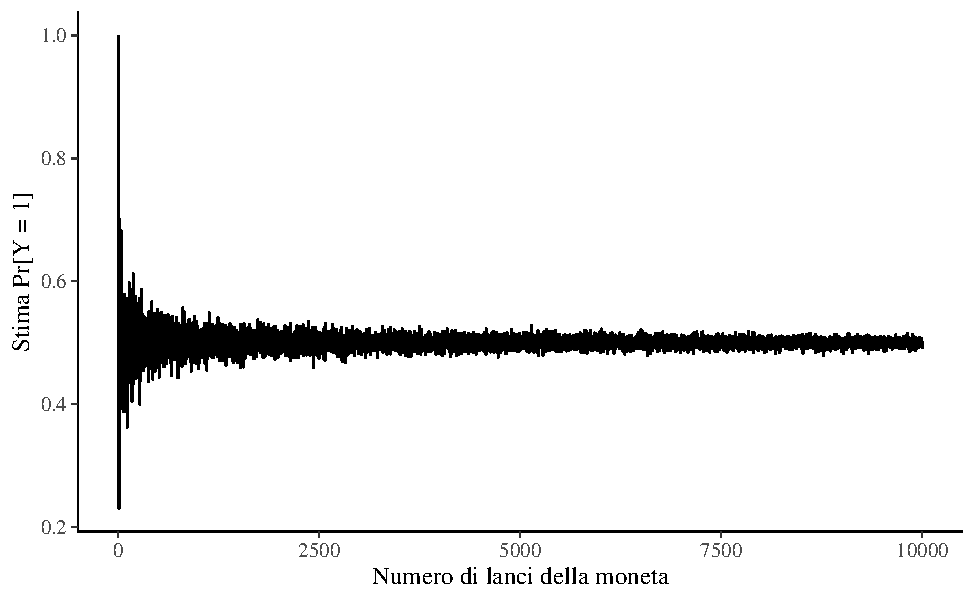
\includegraphics{ds4psy_files/figure-latex/legge-grandi-n-1-1} 

}

\caption{Stima della probabilità di successo in funzione del numero di lanci di una moneta.}\label{fig:legge-grandi-n-1}
\end{figure}

Dato che il grafico \ref{fig:legge-grandi-n-1} su una scala lineare non rivela chiaramente l'andamento della simulazione, utilizzeremo invece un grafico in cui sull'asse \(x\) è stata imposta una scala logaritmica. Con l'asse \(x\) su scala logaritmica, i valori tra 1 e 10 vengono tracciati all'incirca con la stessa ampiezza come nel caso dei valori tra 50 e 700, eccetera.

\begin{Shaded}
\begin{Highlighting}[]
\NormalTok{d }\SpecialCharTok{\%\textgreater{}\%} 
  \FunctionTok{ggplot}\NormalTok{(}
    \FunctionTok{aes}\NormalTok{(}\AttributeTok{x =}\NormalTok{ n, }\AttributeTok{y =}\NormalTok{ estimate)}
\NormalTok{  ) }\SpecialCharTok{+}
  \FunctionTok{geom\_line}\NormalTok{() }\SpecialCharTok{+}
  \FunctionTok{scale\_x\_log10}\NormalTok{(}
    \AttributeTok{breaks =} \FunctionTok{c}\NormalTok{(}\DecValTok{1}\NormalTok{, }\DecValTok{3}\NormalTok{, }\DecValTok{10}\NormalTok{, }\DecValTok{50}\NormalTok{, }\DecValTok{200}\NormalTok{, }
               \DecValTok{700}\NormalTok{, }\DecValTok{2500}\NormalTok{, }\DecValTok{10000}\NormalTok{)}
\NormalTok{  ) }\SpecialCharTok{+}
  \FunctionTok{theme}\NormalTok{(}\AttributeTok{legend.title =} \FunctionTok{element\_blank}\NormalTok{()) }\SpecialCharTok{+}
  \FunctionTok{labs}\NormalTok{(}
    \AttributeTok{x =} \StringTok{"Numero di lanci della moneta"}\NormalTok{, }
    \AttributeTok{y =} \StringTok{"Stima Pr[Y = 1]"}
\NormalTok{)}
\end{Highlighting}
\end{Shaded}

\begin{figure}[h]

{\centering 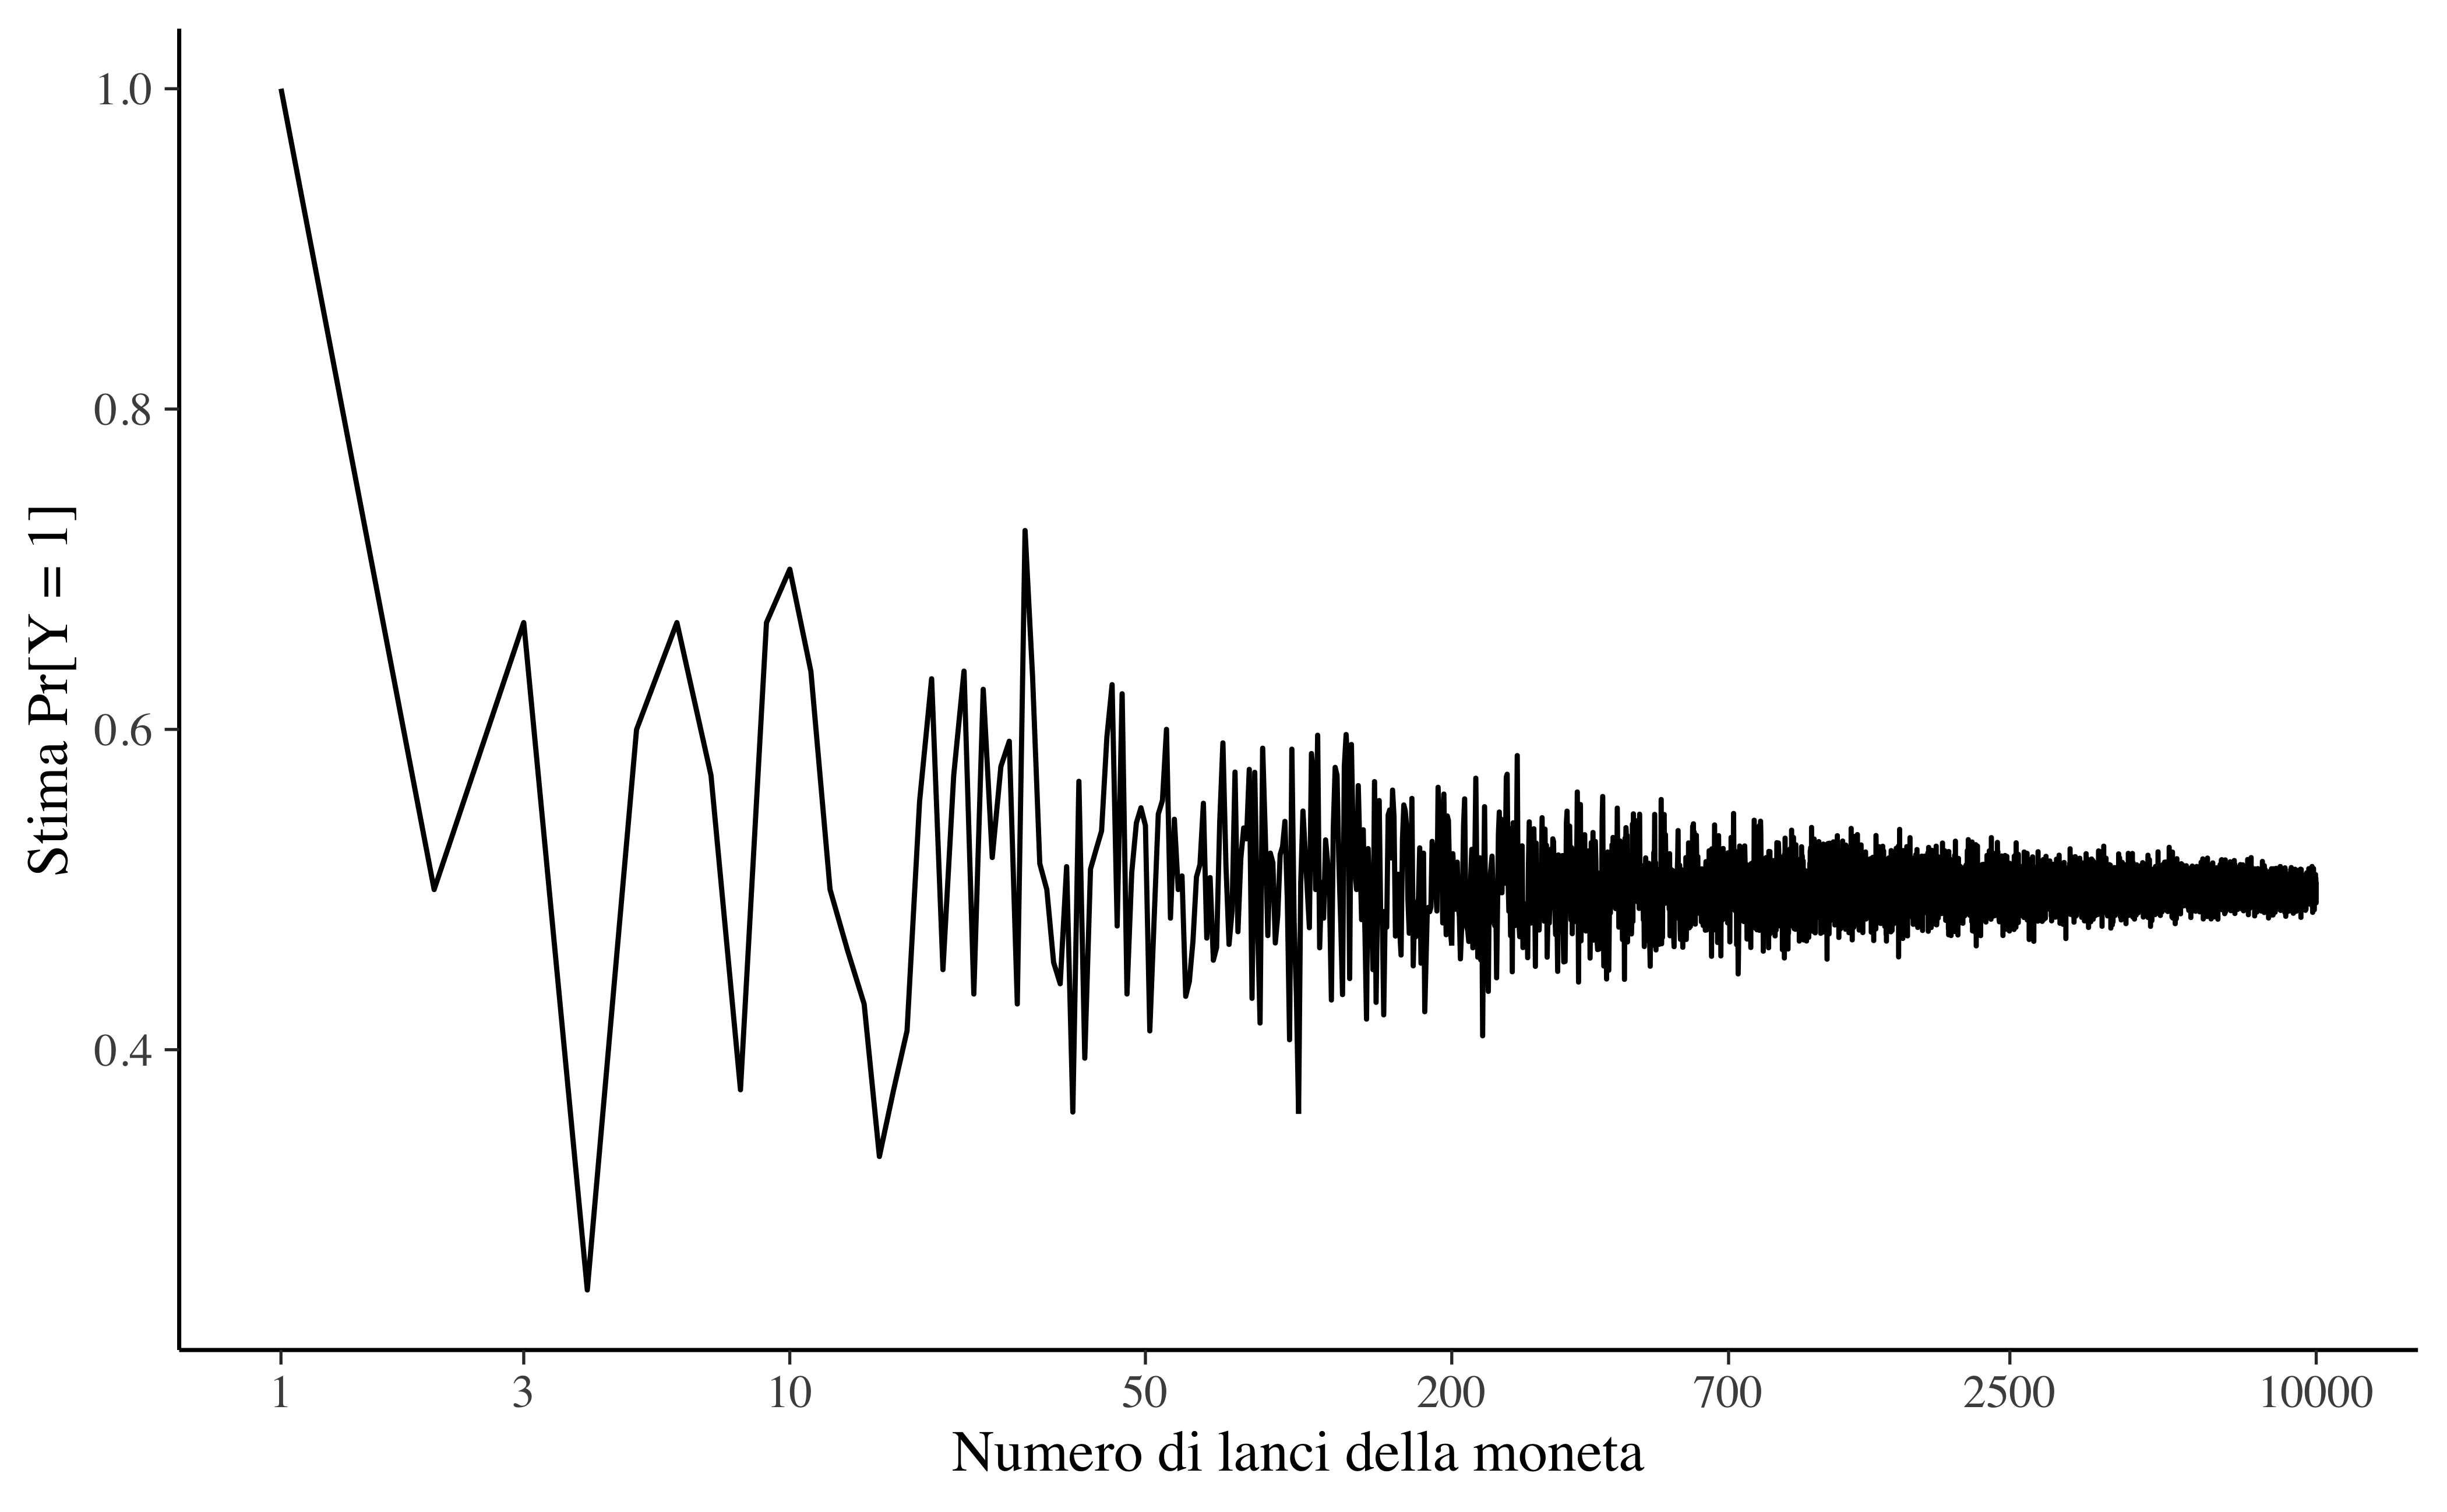
\includegraphics{ds4psy_files/figure-latex/legge-grandi-n-2-1} 

}

\caption{Stima della probabilità di successo in funzione del numero di lanci di una moneta -- scala logaritmica.}\label{fig:legge-grandi-n-2}
\end{figure}

La \emph{legge dei grandi numeri} ci dice che all'aumentare del numero di ripetizioni dell'esperimento casuale la media dei risultati ottenuti tenderà ad avvicinarsi al valore atteso man mano che verranno eseguite più prove. Nel caso presente, la figura \ref{fig:legge-grandi-n-2} mostra appunto che, all'aumentare del numero \emph{M} di lanci della moneta, la stima di \(Pr[Y = 1]\) tende a convergere al vero valore di 0.5.

\hypertarget{variabili-casuali-multiple}{%
\section{Variabili casuali multiple}\label{variabili-casuali-multiple}}

Le variabili casuali non esistono isolatamente. Abbiamo iniziato con una singola variabile casuale \emph{Y} che rappresenta il risultato di un singolo, specifico lancio di una moneta equlibrata. Ma supponiamo ora di lanciare la moneta tre volte. Ciò suggerisce che possiamo avere le variabili casuali \(Y_1 , Y_2 , Y_3\) che rappresentano i risultati di ciascuno dei lanci. Possiamo assumere che ogni lancio sia indipendente, ovvero che non dipenda dal risultato degli altri lanci. Ognuna di queste variabili \(Y_n\) per \(n \in 1:3\) ha \(Pr[Y_n =1]=0.5\) e \(Pr[Y_n =0]=0.5\). Possiamo combinare più variabili casuali usando le operazioni aritmetiche. Se \(Y_1 , Y_2, Y_3\) sono variabili casuali che rappresentano tre lanci di una moneta equilibrata (o un lancio di tre monete equilibrate), possiamo definire la somma di tali variabili casuali come

\[
Z = Y_1 + Y_2 + Y_3.
\] \noindent Possiamo simulare i valori assunti dalla variabile casuale \emph{Z} simulando i valori di \(Y_1, Y_2, Y_3\) per poi sommarli.

\begin{Shaded}
\begin{Highlighting}[]
\NormalTok{y1 }\OtherTok{\textless{}{-}} \FunctionTok{rbinom}\NormalTok{(}\DecValTok{1}\NormalTok{, }\DecValTok{1}\NormalTok{, }\FloatTok{0.5}\NormalTok{)}
\NormalTok{y2 }\OtherTok{\textless{}{-}} \FunctionTok{rbinom}\NormalTok{(}\DecValTok{1}\NormalTok{, }\DecValTok{1}\NormalTok{, }\FloatTok{0.5}\NormalTok{)}
\NormalTok{y3 }\OtherTok{\textless{}{-}} \FunctionTok{rbinom}\NormalTok{(}\DecValTok{1}\NormalTok{, }\DecValTok{1}\NormalTok{, }\FloatTok{0.5}\NormalTok{)}
\FunctionTok{c}\NormalTok{(y1, y2, y3)}
\CommentTok{\#\textgreater{} [1] 0 0 1}
\NormalTok{z }\OtherTok{\textless{}{-}} \FunctionTok{sum}\NormalTok{(}\FunctionTok{c}\NormalTok{(y1, y2, y3))}
\FunctionTok{cat}\NormalTok{(}\StringTok{"z ="}\NormalTok{, z, }\StringTok{"}\SpecialCharTok{\textbackslash{}n}\StringTok{"}\NormalTok{)}
\CommentTok{\#\textgreater{} z = 1}
\end{Highlighting}
\end{Shaded}

\noindent ovvero,

\begin{Shaded}
\begin{Highlighting}[]
\NormalTok{y }\OtherTok{\textless{}{-}} \FunctionTok{rep}\NormalTok{(}\ConstantTok{NA}\NormalTok{, }\DecValTok{3}\NormalTok{)}
\ControlFlowTok{for}\NormalTok{ (i }\ControlFlowTok{in} \DecValTok{1}\SpecialCharTok{:}\DecValTok{3}\NormalTok{) \{}
\NormalTok{  y[i] }\OtherTok{\textless{}{-}} \FunctionTok{rbinom}\NormalTok{(}\DecValTok{1}\NormalTok{, }\DecValTok{1}\NormalTok{, }\FloatTok{0.5}\NormalTok{)}
\NormalTok{\}}
\NormalTok{y}
\CommentTok{\#\textgreater{} [1] 1 0 0}
\NormalTok{z }\OtherTok{\textless{}{-}} \FunctionTok{sum}\NormalTok{(y)}
\FunctionTok{cat}\NormalTok{(}\StringTok{"z ="}\NormalTok{, z, }\StringTok{"}\SpecialCharTok{\textbackslash{}n}\StringTok{"}\NormalTok{)}
\CommentTok{\#\textgreater{} z = 1}
\end{Highlighting}
\end{Shaded}

\noindent oppure, ancora più semplicemente:

\begin{Shaded}
\begin{Highlighting}[]
\NormalTok{y }\OtherTok{\textless{}{-}} \FunctionTok{rbinom}\NormalTok{(}\DecValTok{3}\NormalTok{, }\DecValTok{1}\NormalTok{, }\FloatTok{0.5}\NormalTok{)}
\NormalTok{y}
\CommentTok{\#\textgreater{} [1] 0 1 1}
\NormalTok{z }\OtherTok{\textless{}{-}} \FunctionTok{sum}\NormalTok{(y)}
\FunctionTok{cat}\NormalTok{(}\StringTok{"z ="}\NormalTok{, z, }\StringTok{"}\SpecialCharTok{\textbackslash{}n}\StringTok{"}\NormalTok{)}
\CommentTok{\#\textgreater{} z = 2}
\end{Highlighting}
\end{Shaded}

\noindent Possiamo ripetere questa simulazione \(M = 1e5\) volte:

\begin{Shaded}
\begin{Highlighting}[]
\NormalTok{M }\OtherTok{\textless{}{-}} \FloatTok{1e5}
\NormalTok{z }\OtherTok{\textless{}{-}} \FunctionTok{rep}\NormalTok{(}\ConstantTok{NA}\NormalTok{, M)}
\ControlFlowTok{for}\NormalTok{(i }\ControlFlowTok{in} \DecValTok{1}\SpecialCharTok{:}\NormalTok{M) \{}
\NormalTok{  y }\OtherTok{\textless{}{-}} \FunctionTok{rbinom}\NormalTok{(}\DecValTok{3}\NormalTok{, }\DecValTok{1}\NormalTok{, }\FloatTok{0.5}\NormalTok{)}
\NormalTok{  z[i] }\OtherTok{\textless{}{-}} \FunctionTok{sum}\NormalTok{(y)}
\NormalTok{\}}
\end{Highlighting}
\end{Shaded}

\noindent e calcolare una stima della probabilità che la variabile casuale \(Z\) assuma i valori 0, 1, 2, 3:

\begin{Shaded}
\begin{Highlighting}[]
\FunctionTok{table}\NormalTok{(z) }\SpecialCharTok{/}\NormalTok{ M}
\CommentTok{\#\textgreater{} z}
\CommentTok{\#\textgreater{}      0      1      2      3 }
\CommentTok{\#\textgreater{} 0.1256 0.3750 0.3749 0.1245}
\end{Highlighting}
\end{Shaded}

Nel caso di 4 monete equilibrate, avremo:

\begin{Shaded}
\begin{Highlighting}[]
\NormalTok{M }\OtherTok{\textless{}{-}} \FloatTok{1e5}
\NormalTok{z }\OtherTok{\textless{}{-}} \FunctionTok{rep}\NormalTok{(}\ConstantTok{NA}\NormalTok{, M)}
\ControlFlowTok{for}\NormalTok{(i }\ControlFlowTok{in} \DecValTok{1}\SpecialCharTok{:}\NormalTok{M) \{}
\NormalTok{  y }\OtherTok{\textless{}{-}} \FunctionTok{rbinom}\NormalTok{(}\DecValTok{4}\NormalTok{, }\DecValTok{1}\NormalTok{, }\FloatTok{0.5}\NormalTok{)}
\NormalTok{  z[i] }\OtherTok{\textless{}{-}} \FunctionTok{sum}\NormalTok{(y)}
\NormalTok{\}}
\FunctionTok{table}\NormalTok{(z) }\SpecialCharTok{/}\NormalTok{ M}
\CommentTok{\#\textgreater{} z}
\CommentTok{\#\textgreater{}       0       1       2       3       4 }
\CommentTok{\#\textgreater{} 0.06213 0.25019 0.37400 0.25097 0.06271}
\end{Highlighting}
\end{Shaded}

Viene detta \emph{variabile casuale discreta} una variabile casuale le cui modalità possono essere costituite solo da numeri interi:

\[
\mathbb{Z} = \dots, -2, -1, 0, 1, 2, \dots
\]

\hypertarget{sec:fun-mass-prob}{%
\section{Funzione di massa di probabilità}\label{sec:fun-mass-prob}}

È conveniente avere una funzione che associa ogni possibile valore di una variabile casuale alla sua probabilità. In generale, ciò è possibile se e solo se la variabile casuale è discreta, così com'è stata definita nel Paragrafo precedente.

Ad esempio, se consideriamo \(Z = Y_1 + \dots + Y_4\) come il numero di risultati ``testa'' in 4 lanci della moneta, allora possiamo definire la seguente funzione:

\[
\begin{array}{rclll}
p_Z(0) & = & 1/16 & & \mathrm{TTTT}
\\
p_Z(1) & = & 4/16 & & \mathrm{HTTT, THTT, TTHT, TTTH}
\\
p_Z(2) & = & 6/16 & & \mathrm{HHTT, HTHT, HTTH, THHT, THTH, TTTH}
\\
p_Z(3) & = & 4/16 & & \mathrm{HHHT, HHTH, HTHH, THHH}
\\
p_Z(4) & = & 1/16 & & \mathrm{HHHH}
\end{array}
\]

Il lancio di quattro monete può produrre sedici possibili risultati. Dato che i lanci sono indipendenti e le monete sono equilibrate, ogni possibile risultato è ugualmente probabile. Nella tabella in alto, le sequenze dei risultati possibili del lancio delle 4 monete sono riportate nella colonna più a destra. Le probabilità si ottengono dividendo il numero di sequenze che producono lo stesso numero di eventi testa per il numero dei risultati possibili.

La funzione \(p_Z\) è stata costruita per mappare un valore \(u\) per \(Z\) alla probabilità dell'evento \(Z = u\). Convenzionalmente, queste probabilità sono scritte come

\[
p_Z(z) = \mbox{Pr}[Z = z].
\]

La parte a destra dell'uguale si può leggere come: ``la probabilità che la variabile casuale \(Z\) assuma il valore \(z\)''.

Una funzione definita come sopra è detta \emph{funzione di massa di probabilità} della variabile casuale \(Z\). Ad ogni variabile casuale discreta è associata un'unica funzione di massa di probabilità.

Una rappresentazione grafica della stima della funzione di massa di probabilità per l'esperimento casuale del lancio di quattro monete equilibrate è fornita nella figura \ref{fig:barplot-mdf-4coins}.

\begin{Shaded}
\begin{Highlighting}[]
\FunctionTok{set.seed}\NormalTok{(}\DecValTok{1234}\NormalTok{)}
\NormalTok{M }\OtherTok{\textless{}{-}} \FloatTok{1e5}
\NormalTok{nflips }\OtherTok{\textless{}{-}} \DecValTok{4}
\NormalTok{u }\OtherTok{\textless{}{-}} \FunctionTok{rbinom}\NormalTok{(M, nflips, }\FloatTok{0.5}\NormalTok{)}
\NormalTok{x }\OtherTok{\textless{}{-}} \DecValTok{0}\SpecialCharTok{:}\NormalTok{nflips}
\NormalTok{y }\OtherTok{\textless{}{-}} \FunctionTok{rep}\NormalTok{(}\ConstantTok{NA}\NormalTok{, nflips}\SpecialCharTok{+}\DecValTok{1}\NormalTok{)}
\ControlFlowTok{for}\NormalTok{ (n }\ControlFlowTok{in} \DecValTok{0}\SpecialCharTok{:}\NormalTok{nflips)}
\NormalTok{  y[n }\SpecialCharTok{+} \DecValTok{1}\NormalTok{] }\OtherTok{\textless{}{-}} \FunctionTok{sum}\NormalTok{(u }\SpecialCharTok{==}\NormalTok{ n) }\SpecialCharTok{/}\NormalTok{ M}
\NormalTok{bar\_plot }\OtherTok{\textless{}{-}}
  \FunctionTok{data.frame}\NormalTok{(}\AttributeTok{Z =}\NormalTok{ x, }\AttributeTok{count =}\NormalTok{ y) }\SpecialCharTok{\%\textgreater{}\%} 
  \FunctionTok{ggplot}\NormalTok{(}
    \FunctionTok{aes}\NormalTok{(}\AttributeTok{x =}\NormalTok{ Z, }\AttributeTok{y =}\NormalTok{ count)}
\NormalTok{  ) }\SpecialCharTok{+}
  \FunctionTok{geom\_bar}\NormalTok{(}\AttributeTok{stat =} \StringTok{"identity"}\NormalTok{) }\SpecialCharTok{+}
  \FunctionTok{scale\_x\_continuous}\NormalTok{(}
    \AttributeTok{breaks =} \DecValTok{0}\SpecialCharTok{:}\DecValTok{4}\NormalTok{,}
    \AttributeTok{labels =} \FunctionTok{c}\NormalTok{(}\DecValTok{0}\NormalTok{, }\DecValTok{1}\NormalTok{, }\DecValTok{2}\NormalTok{, }\DecValTok{3}\NormalTok{, }\DecValTok{4}\NormalTok{)}
\NormalTok{  ) }\SpecialCharTok{+}
  \FunctionTok{labs}\NormalTok{(}
    \AttributeTok{y =} \StringTok{"Probabilità stimata Pr[Z = z]"}
\NormalTok{)}
\NormalTok{bar\_plot}
\end{Highlighting}
\end{Shaded}

\begin{figure}[h]

{\centering 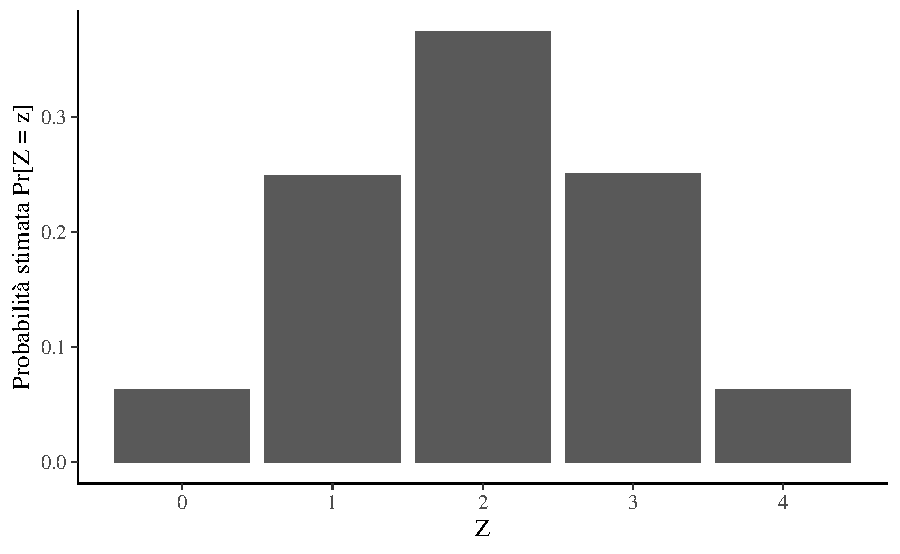
\includegraphics{ds4psy_files/figure-latex/barplot-mdf-4coins-1} 

}

\caption{Grafico di $M = 100\,000$ simulazioni della funzione di massa di probabilità di una variabile casuale definita come il numero di teste in quattro lanci di una moneta equilibrata.}\label{fig:barplot-mdf-4coins}
\end{figure}

Se \(A\) è un sottoinsieme della variabile casuale \(Z\), allora denotiamo con \(P_{z}(A)\) la probabilità assegnata ad \(A\) dalla distribuzione \(P_{z}\). Mediante una distribuzione di probabilità \(P_{z}\) è dunque possibile determinare la probabilità di ciascun sottoinsieme \(A \subset Z\) come

\[
P_{z}(A) = \sum_{z \in A} P_{z}(Z).
\]

\begin{example}
Nel caso dell'esempio discusso nella Sezione \ref{sec:fun-mass-prob}, la probabilità che la variabile casuale \(Z\) sia un numero dispari è \[
Pr(\text{Z è un numero dispari}) = P_{z}(Z = 1) + P_{z}(Z = 3) = \frac{4}{16} + \frac{4}{16} = \frac{1}{2}.
\]
\end{example}

\hypertarget{considerazioni-conclusive}{%
\section*{Considerazioni conclusive}\label{considerazioni-conclusive}}


In questo capitolo abbiamo visto come si costruisce lo spazio campionario di un esperimento casuale, quali sono le proprietà di base della probabilità e come si assegnano le probabilità agli eventi definiti sopra uno spazio campionario discreto. Abbiamo anche introdotto le nozioni di ``variabile casuale'', ovvero di una variabile che prende i suoi valori casualmente. E abbiamo descritto il modo di specificare la probabilità con cui sono presi i differenti valori, ovvero la funzione di distribuzione probabilistica \(F(X) = Pr(X < x)\), e la funzione di massa di probabilità. Le procedure di analisi dei dati psicologici che discuteremo in seguito faranno un grande uso di questi concetti e della notazione qui introdotta.

\hypertarget{chapter-ppc}{%
\chapter{Distribuzione predittiva a posteriori}\label{chapter-ppc}}

Oltre ad una sintesi della distribuzione a posteriori attraverso il computo di indici caratteristici e alla verifica di ipotesi, un altro compito dell'analisi bayesiana è la predizione di nuovi dati futuri. Dopo aver osservato i dati di un campione e ottenuto le distribuzioni a posteriori dei parametri, è infatti possibile ottenere una qualche indicazione su come potrebbero essere i dati futuri. L'uso più immediato della stima della distribuzione dei possibili valori futuri della variabile di esito è la verifica del modello. Infatti, il modo più diretto per testare un modello è quello di utilizzare il modello per fare previsioni sui possibili dati futuri per poi confrontare i dati predetti con i dati effettivi. Questa pratica va sotto il nome di controllo predittivo a posteriori.

\hypertarget{la-distribuzione-dei-possibili-valori-futuri}{%
\section{La distribuzione dei possibili valori futuri}\label{la-distribuzione-dei-possibili-valori-futuri}}

La distribuzione dei possibili valori futuri della variabile di esito può essere predetta da un modello statistico sulla base della distribuzione a posteriori dei parametri, \(p(\theta \mid y)\), avendo già osservato \(n\) manifestazioni del fenomeno \(y\). Una tale distribuzione va sotto il nome di \emph{distribuzione predittiva a posteriori} (\emph{posterior predictive distribution}, PPD).

Quando vengono simulate le osservazioni della distribuzione predittiva a posteriori si usa la notazione \(y^{rep}\) (dove \(rep\) sta per \emph{replica}) quando, nella simulazione, vengono utilizzate le stesse osservazioni di \(X\) che erano state usate per stimare i parametri del modello. Si usa invece la notazione \(\tilde{y}\) per fare riferimento a possibili valori \(X\) che non sono contenuti nel campione osservato, ovvero, ad un campione di dati che potrebbe essere osservato in qualche futura occasione.

La distribuzione predittiva a posteriori viene usata per fare inferenze predittive. L'idea è che, se il modello ben si adatta bene ai dati del campione allora, sulla base dei parametri stimati, dovremmo essere in grado di generare nuovi dati non osservati \(y^{rep}\) che risultano molto simili ai dati osservati \(y\). I dati \(y^{rep}\) vengono concepiti come stime di \(\tilde{y}\). La distribuzione predittiva a posteriorie è data da:

\begin{equation}
p(\tilde{y} \mid y) = \int_{\theta} p(\tilde{y}, \theta \mid y) d \theta = \int_{\theta} p(\tilde{y} \mid \theta, y) p(\theta \mid y) d\theta.\notag
\end{equation}

Supponendo che le osservazioni passate e future siano condizionalmente indipendenti dato \(\theta\), ovvero che \(p(\tilde{y} \mid \theta, y) = p(\tilde{y} \mid \theta)\), possiamo scrivere

\begin{equation}
p(\tilde{y} \mid y) = \int_{\theta} p(\tilde{y} \mid \theta) p(\theta \mid y) d\theta.
\label{eq:dist-pred-post}
\end{equation}

La \eqref{eq:dist-pred-post} descrive la nostra incertezza sulla distribuzione di future osservazioni di dati, data la distribuzione a posteriori di \(\theta\), ovvero tenendo conto della scelta del modello e della stima dei parametri mediante i dati osservati. Si noti che, nella \eqref{eq:dist-pred-post}, \(\tilde{y}\) è condizionato da \(y\) ma non da ciò che è incognito, ovvero \(\theta\). La distribuzione predittiva a posteriori è invece ottenuta mediante marginalizzazione sopra le variabili da ``scartare'', ovvero sopra i parametri incogniti \(\theta\).

Un esempio formulato mediante il codice Stan può chiarire questo concetto. Consideriamo il codice relativo alla distribuzione predittiva a posteriori nel caso di un modello di regressione lineare classico con un solo predittore \(x\). Il blocco \emph{Model} sarà:

\begin{Shaded}
\begin{Highlighting}[]
\NormalTok{model \{}
\NormalTok{ y }\SpecialCharTok{\textasciitilde{}} \FunctionTok{normal}\NormalTok{(x }\SpecialCharTok{*}\NormalTok{ beta }\SpecialCharTok{+}\NormalTok{ alpha, sigma);}
\NormalTok{\}}
\end{Highlighting}
\end{Shaded}

Quello che è di interesse per la discussione presente è il blocco \emph{Generated Quantities}. Tale blocco avrà questa forma:

\begin{Shaded}
\begin{Highlighting}[]
\NormalTok{generated quantities \{}
\NormalTok{ real y\_rep[N];}
 \ControlFlowTok{for}\NormalTok{ (n }\ControlFlowTok{in} \DecValTok{1}\SpecialCharTok{:}\NormalTok{N) \{}
\NormalTok{   y\_rep[n] }\OtherTok{=} \FunctionTok{normal\_rng}\NormalTok{(x[n] }\SpecialCharTok{*}\NormalTok{ beta }\SpecialCharTok{+}\NormalTok{ alpha, sigma);}
\NormalTok{ \}}
\NormalTok{\}}
\end{Highlighting}
\end{Shaded}

La variabile \texttt{y\_rep} è ciò a cui siamo interessati. Nel codice precedente, \texttt{x} è il vettore che contiene i valori della variabile indipendente nel campione di osservazioni esaminato. I parametri del modello di regressione sono \texttt{alpha} e \texttt{beta}; \texttt{sigma} è la stima dell'errore standard della regressione. Supponiamo che questi tre parametri siano degli scalari. Se lo fossero, per il valore \texttt{x} \(n\)-esimo, l'istruzione \texttt{normal\_rng()} ritornerebbe un valore a caso dalla distribuzione normale con media \(\alpha + \beta x_n\) e deviazione standard \(\sigma\). Il ciclo \texttt{for()} ripete questa operazione \(N\) volte, ovvero tante volte quanti sono gli elementi del vettore \texttt{x} del campione. Quello che è stato detto sopra ci dà un'idea di quello che succederebbe se \texttt{alpha}, \texttt{beta} e \texttt{sigma} fossero degli scalari. Ma non lo sono. Per ciascuno dei tre paramatri abbiamo un numero molto alto di stime, ovvero l'approssimazione MCMC della distribuzione a posteriori. Poniamo che l'ampiezza campionaria \(N\) sia 30. Se \texttt{alpha}, \texttt{beta} e \texttt{sigma} fossero degli scalari, la distribuzione predittiva a posteriori sarebbe costituita da 30 valori \(y^{rep}\), ovvero, non sarebbe nient'altro che \(\hat{y} = \hat{\alpha} + \hat{\beta} x\). Ma \texttt{alpha}, \texttt{beta} e \texttt{sigma} non sono degli scalari: per ciascuno di questi parametri abbiamo un grande numero di stime, diciamo 2000. Dunque, quando \texttt{normal\_rng()} estrae un valore a caso dalla distribuzione normale, i parametri della normale non sono fissi: per determinare \(\mu\) prendiamo un valore a caso, chiamiamolo \texttt{beta\textquotesingle{}}, dalla distribuzione dei valori \texttt{beta} e un valore a caso, chiamiamolo \texttt{alpha\textquotesingle{}}, dalla distribuzione dei valori \texttt{alpha}. Avendo questi due valori, calcoliamo il valore \(\mu'_n = \alpha' + \beta' x_n\). Lo stesso si può dire per \(\sigma'\). A questo punto possiamo trovare il valore \texttt{y\_n\textquotesingle{}} estraendo un valore a caso dalla distribuzione gaussiana di parametri \(\mu'\) e \(\sigma'\). Per l'\(n\)-esimo valore \(x\) possiamo ripetere questo processo tante volte. Se lo ripetiamo, ad esempio, 2,000 volte, per tutti e 30 i valori \(x\) del campione otterremo una matrice \(30 \times 2,000\). In questo modo possiamo generare le previsioni del modello, ovvero \(y^{rep}\), che includono due fonti di incertezza:

\begin{itemize}
\tightlist
\item
  la variabilità campionaria, ovvero il fatto che abbiamo osservato uno specifico insieme di valori \((x, y)\); in un altro campione tali valori saranno diversi;
\item
  la variabilità a posteriori della distribuzione dei parametri, ovvero il fatto che di ciascun parametro non conosciamo il ``valore vero'' ma solo una distribuzione (a posteriori) di valori.
\end{itemize}

Nel caso dell'esempio presente, l'integrale della \eqref{eq:dist-pred-post} può essere interpretato dicendo che, nell'esempio della matrice di dimensioni \(30 \times 2,000\), noi marginalizziamo rispetto alle colonne, ovvero, per ciascuna riga facciamo la media dei valori colonna. Otteniamo così un vettore di 30 osservazioni, ovvero \(y^{rep}\).

Quando, con metodi grafici, vengono esaminati i valori della distribuzione predittiva a posteriori, possiamo esaminare un numero arbitrario di previsioni. Per esempio, possiamo rappresentare graficamente 50 rette di regressione predette -- o un qualsiasi altro numero. Questa rappresentazione grafica quantifica la nostra incertezza a posteriori relativamente (in questo esempio) all'orientamento della retta di regressione.

\begin{exercise}
Illustreremo ora il problema di trovare la distribuzione \(p(\tilde{y} \mid y)\) in un caso semplice, ovvero quello dello schema Beta-Binomiale. Nell'esempio, useremo un'altra volta i dati del campione di pazienti clinici depressi di \citet{zetschefuture2019} -- si veda l'Appendice \ref{es-pratico-zetsche}. Supponendo di volere esaminare in futuro altri 30 pazienti clinici, ci chiediamo: quanti di essi manifesteranno una depressione grave?

Se vogliamo fare predizioni su \(\tilde{y}\) (il numero di ``successi'' previsti futuri) dobbiamo innanzitutto riconoscere che i possibili valori \(\tilde{y} \in \{0, 1, \dots, 30\}\) non sono tutti egualmente plausibili. Sappiamo che \(\tilde{y}\) è una v.c. binomiale con distribuzione

\begin{equation}
p(\tilde{y}\mid \theta) = \binom{30}{\tilde{y}} \theta^{\tilde{y}}(1-\theta)^{30 - \tilde{y}} \; .
\label{eq:post-yprime}
\end{equation}

La v.c. \(\tilde{y}\) dipende da \(\theta\), ma il parametro \(\theta\) è esso stesso una variabile casuale. Avendo osservato \(y = 23\) successi in \(n = 30\) prove nel campione (laddove la presenza di una depressione grave è stata considerata un ``successo''), e avendo assunto come distribuzione a priori per \(\theta\) una \(\mbox{Beta}(2, 10)\) (per continuare con l'esempio precedente), la distribuzione a posteriori di \(\theta\) sarà una \(\mbox{Beta}(25, 17)\):

\begin{Shaded}
\begin{Highlighting}[]
\NormalTok{bayesrules}\SpecialCharTok{::}\FunctionTok{summarize\_beta\_binomial}\NormalTok{(}
  \AttributeTok{alpha =} \DecValTok{2}\NormalTok{, }\AttributeTok{beta =} \DecValTok{10}\NormalTok{, }\AttributeTok{y =} \DecValTok{23}\NormalTok{, }\AttributeTok{n =} \DecValTok{30}
\NormalTok{)}
\CommentTok{\#\textgreater{}       model alpha beta   mean mode      var      sd}
\CommentTok{\#\textgreater{} 1     prior     2   10 0.1667  0.1 0.010684 0.10336}
\CommentTok{\#\textgreater{} 2 posterior    25   17 0.5952  0.6 0.005603 0.07485}
\end{Highlighting}
\end{Shaded}

Per trovare la distribuzione sui possibili dati previsti futuri \(\tilde{y}\) dobbiamo applicare la \eqref{eq:dist-pred-post}:

\begin{align}
p(\tilde{y} \mid y = 23) = \int_0^1 p(\tilde{y} \mid \theta) p(\theta \mid y = 23) d\theta \; .
\label{eq:post-yprime-y17}
\end{align}

Per il modello Beta-Binomiale è possibile trovare una soluzione analitica alla \eqref{eq:dist-pred-post}.

Poniamo di avere osservato \(y\) successi in \(n\) prove e di utilizzare una distribuzione a priori \(\mbox{Beta}(a, b)\). Possiamo scrivere

\begin{align}
p(\tilde{y} \mid y) &= \int_0^1 p(\tilde{y} \mid \theta)
p(\theta \mid y)\, d\theta \notag\\
 &= \int_0^1 \begin{pmatrix}\tilde{n}\\\tilde{y}\end{pmatrix}
 \theta^{\tilde{y}}
(1-\theta)^{\tilde{n}-\tilde{y}} \mbox{Beta}(a+y,b+n-y) \, d\theta \notag\\
&= \begin{pmatrix}{\tilde{n}}\\\tilde{y}\end{pmatrix} \int_0^1 \theta^{\tilde{y}}
(1-\theta)^{\tilde{n}-\tilde{y}} \frac{1}{B(a+y, b+n-y)}\theta^{a+y-1}(1-\theta)^{b+n-y-1}\notag\\
&= \begin{pmatrix}{\tilde{n}}\\\tilde{y}\end{pmatrix} \frac{1}{B(a+y, b+n-y)}\int_0^1 \theta^{\tilde{y}+a+y-1}(1-\theta)^{\tilde{n}-\tilde{y}+b+n-y-1}\notag\\
&= \begin{pmatrix}{\tilde{n}}\\\tilde{y}\end{pmatrix} \frac{B(\tilde{y}+a+y,b+n-y+\tilde{n}-\tilde{y})}{B(a+y, b+n-y)} \; .
\label{eq:post-yprime-an-sol-betabin}
\end{align}

Svolgendo i calcoli in \(\R\), per i dati dell'esempio otteniamo:

\begin{Shaded}
\begin{Highlighting}[]
\NormalTok{beta\_binom }\OtherTok{\textless{}{-}} \ControlFlowTok{function}\NormalTok{(rp) \{}
\NormalTok{  val }\OtherTok{\textless{}{-}} \FunctionTok{choose}\NormalTok{(np, rp) }\SpecialCharTok{*}
    \FunctionTok{beta}\NormalTok{(rp }\SpecialCharTok{+}\NormalTok{ a }\SpecialCharTok{+}\NormalTok{ y, b }\SpecialCharTok{+}\NormalTok{ n }\SpecialCharTok{{-}}\NormalTok{ y }\SpecialCharTok{+}\NormalTok{ np }\SpecialCharTok{{-}}\NormalTok{ rp) }\SpecialCharTok{/}
    \FunctionTok{beta}\NormalTok{(a }\SpecialCharTok{+}\NormalTok{ y, b }\SpecialCharTok{+}\NormalTok{ n }\SpecialCharTok{{-}}\NormalTok{ y)}
\NormalTok{  val}
\NormalTok{\}}

\NormalTok{n }\OtherTok{\textless{}{-}} \DecValTok{30}
\NormalTok{y }\OtherTok{\textless{}{-}} \DecValTok{23}
\NormalTok{a }\OtherTok{\textless{}{-}} \DecValTok{2}
\NormalTok{b }\OtherTok{\textless{}{-}} \DecValTok{10}
\NormalTok{np }\OtherTok{\textless{}{-}} \DecValTok{30}
\FunctionTok{data.frame}\NormalTok{(}
  \AttributeTok{heads =} \DecValTok{0}\SpecialCharTok{:}\NormalTok{np,}
  \AttributeTok{pmf =} \FunctionTok{beta\_binom}\NormalTok{(}\DecValTok{0}\SpecialCharTok{:}\NormalTok{np)}
\NormalTok{) }\SpecialCharTok{\%\textgreater{}\%}
  \FunctionTok{ggplot}\NormalTok{(}\FunctionTok{aes}\NormalTok{(}\AttributeTok{x =} \FunctionTok{factor}\NormalTok{(heads), }\AttributeTok{y =}\NormalTok{ pmf)) }\SpecialCharTok{+}
  \FunctionTok{geom\_col}\NormalTok{() }\SpecialCharTok{+}
  \FunctionTok{labs}\NormalTok{(}
    \AttributeTok{title =} \StringTok{"Distribuzione predittiva a posteriori"}\NormalTok{,}
    \AttributeTok{x =} \StringTok{"y\textquotesingle{}"}\NormalTok{,}
    \AttributeTok{y =} \StringTok{"P(Y = y\textquotesingle{} | Data)"}
\NormalTok{  )}
\end{Highlighting}
\end{Shaded}

\begin{center}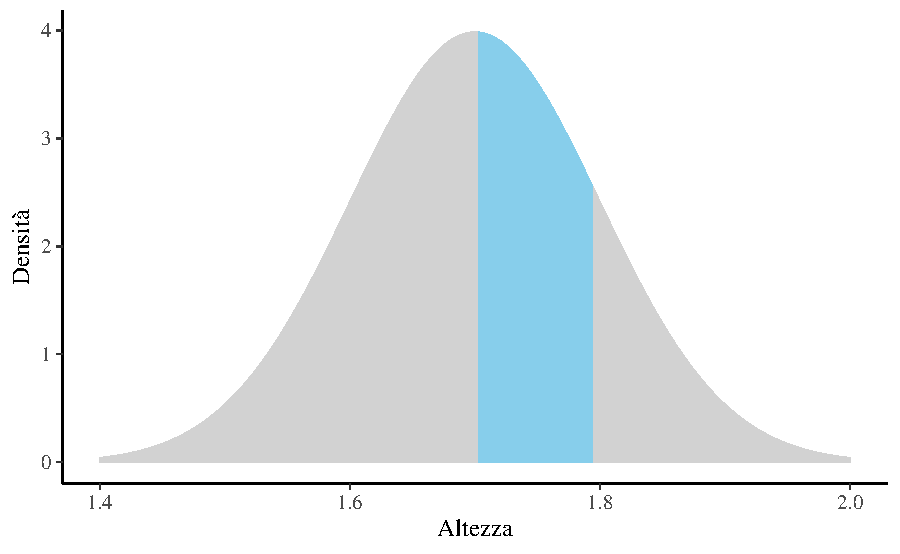
\includegraphics{ds4psy_files/figure-latex/unnamed-chunk-22-1} \end{center}

\noindent È facile vedere come, in questo esempio, la distribuzione predittiva a posteriori \(p(\tilde{y} \mid y)\) sia diversa dalla binomiale di parametro \(\theta = 23/30\):

\begin{Shaded}
\begin{Highlighting}[]
\FunctionTok{tibble}\NormalTok{(}
  \AttributeTok{heads =} \DecValTok{0}\SpecialCharTok{:}\NormalTok{np,}
  \AttributeTok{pmf =} \FunctionTok{dbinom}\NormalTok{(}\AttributeTok{x =} \DecValTok{0}\SpecialCharTok{:}\NormalTok{np, }\AttributeTok{size =}\NormalTok{ np, }\AttributeTok{prob =} \DecValTok{23} \SpecialCharTok{/} \DecValTok{30}\NormalTok{)}
\NormalTok{) }\SpecialCharTok{\%\textgreater{}\%}
  \FunctionTok{ggplot}\NormalTok{(}\FunctionTok{aes}\NormalTok{(}\AttributeTok{x =} \FunctionTok{factor}\NormalTok{(heads), }\AttributeTok{y =}\NormalTok{ pmf)) }\SpecialCharTok{+}
  \FunctionTok{geom\_col}\NormalTok{() }\SpecialCharTok{+}
  \FunctionTok{labs}\NormalTok{(}
    \AttributeTok{title =} \StringTok{"p(y | theta = 0.77)"}\NormalTok{,}
    \AttributeTok{x =} \StringTok{"y"}\NormalTok{,}
    \AttributeTok{y =} \StringTok{"Probabilità"}
\NormalTok{  )}
\end{Highlighting}
\end{Shaded}

\begin{center}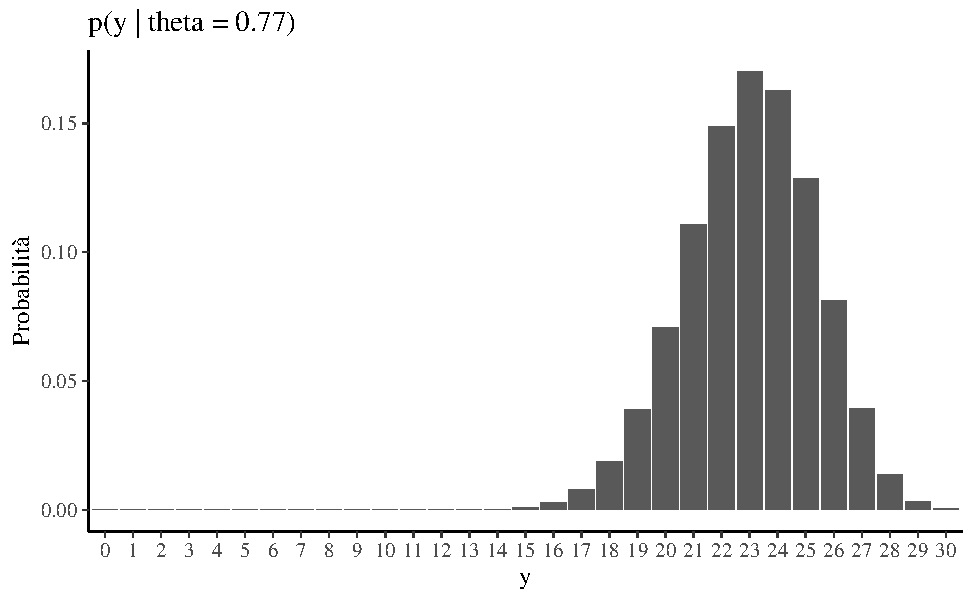
\includegraphics{ds4psy_files/figure-latex/unnamed-chunk-23-1} \end{center}

\noindent In particolare, la \(p(\tilde{y} \mid y)\) ha una varianza maggiore di \(\Bin(y \mid \theta = 0.77, n = 30)\). Questa maggiore varianza riflette le due fonti di incertezza che sono presenti nella \eqref{eq:dist-pred-post}: l'incertezza sul valore del parametro (descritta dalla distribuzione a posteriori) e l'incertezza dovuta alla variabilità campionaria (descritta dalla funzione di verosimiglianza). Possiamo concludere la discussione di questo esempio dicendo che, nel caso di 30 nuovi pazienti clinici, alla luce delle nostre credenze precedenti e dei dati osservati nel campione, ci aspettiamo di osservare 18 pazienti con una depressione severa, anche se è ragionevole aspettarci un numero compreso, diciamo, tra 10 e 25.

Una volta trovata la distribuzione predittiva a posteriori \(p(\tilde{y} \mid y)\) diventa possibile rispondere a domande come: qual è la probabilità di depressione grave in almeno 10 dei 30 pazienti futuri? Rispondere a domande di questo tipo è possibile, ma richiede un po' di lavoro. Tuttavia, non è importante imparare scrivere il codice necessario a risolvere problemi di questo tipo perché, in generale, anche per problemi solo leggermente più complessi di quello discusso qui, non sono disponibili espressioni analitiche della distribuzione predittiva a posteriori. Invece, è possibile trovare una approssimazione numerica della \(p(\tilde{y} \mid y)\) mediante simulazioni MCMC. Inoltre, se viene utilizzato un tale metodo, risulta facile rispondere a domande simili a quella che abbiamo presentato sopra.
\end{exercise}

\hypertarget{metodi-mcmc-per-la-distribuzione-predittiva-a-posteriori}{%
\section{Metodi MCMC per la distribuzione predittiva a posteriori}\label{metodi-mcmc-per-la-distribuzione-predittiva-a-posteriori}}

Se svolgiamo l'analisi bayesiana con il metodo MCMC, le repliche \(p(y^{rep} \mid y)\) (ovvero le stime delle possibili osservazioni future \(p(\tilde{y} \mid y)\)) possono essere ottenute nel modo seguente:

\begin{itemize}
\tightlist
\item
  campionare \(\theta_i \sim p(\theta \mid y)\), ovvero campionare un valore del parametro dalla distribuzione a posteriori;
\item
  campionare \(y^{rep} \sim p(y^{rep} \mid \theta_i)\), ovvero campionare il valore di un'osservazione dalla funzione di verosimiglianza condizionata al valore del parametro definito nel passo precedente.
\end{itemize}

\noindent Se i due passaggi descritti sopra vengono ripetuti un numero sufficiente di volte, l'istogramma risultante approssimerà la distribuzione predittiva a posteriori che, in teoria (ma non in pratica) potrebbe essere ottenuta per via analitica (si veda il Paragrafo \ref{schema-beta-bin-distr-pred-post}).

\begin{exercise}

Generiamo ora \(p(y^{rep} \mid y)\) nel caso dell'inferenza su una proporzione.

Riportiamo qui sotto il codice Stan --- si veda il Capitolo \ref{mod-binom}.

\begin{Shaded}
\begin{Highlighting}[]
\NormalTok{modelString }\OtherTok{=} \StringTok{"}
\StringTok{data \{}
\StringTok{  int\textless{}lower=0\textgreater{} N;}
\StringTok{  int\textless{}lower=0, upper=1\textgreater{} y[N];}
\StringTok{\}}
\StringTok{parameters \{}
\StringTok{  real\textless{}lower=0, upper=1\textgreater{} theta;}
\StringTok{\}}
\StringTok{model \{}
\StringTok{  theta \textasciitilde{} beta(2, 10);}
\StringTok{  y \textasciitilde{} bernoulli(theta);}
\StringTok{\}}
\StringTok{generated quantities \{}
\StringTok{  int y\_rep[N];}
\StringTok{  real log\_lik[N];}
\StringTok{  for (n in 1:N) \{}
\StringTok{    y\_rep[n] = bernoulli\_rng(theta);}
\StringTok{    log\_lik[n] = bernoulli\_lpmf(y[n] | theta);}
\StringTok{  \}}
\StringTok{\}}
\StringTok{"}
\FunctionTok{writeLines}\NormalTok{(modelString, }\AttributeTok{con =} \StringTok{"code/betabin23{-}30{-}2{-}10.stan"}\NormalTok{)}
\end{Highlighting}
\end{Shaded}

\noindent Si noti che nel nel blocco \texttt{generated\ quantities} sono state aggiunte le istruzioni necessarie per simulare \(y^{rep}\), ovvero, \texttt{y\_rep{[}n{]}\ =\ bernoulli\_rng(theta)}. I dati dell'esempio sono:

\begin{Shaded}
\begin{Highlighting}[]
\NormalTok{data\_list }\OtherTok{\textless{}{-}} \FunctionTok{list}\NormalTok{(}
  \AttributeTok{N =} \DecValTok{30}\NormalTok{,}
  \AttributeTok{y =} \FunctionTok{c}\NormalTok{(}\FunctionTok{rep}\NormalTok{(}\DecValTok{1}\NormalTok{, }\DecValTok{23}\NormalTok{), }\FunctionTok{rep}\NormalTok{(}\DecValTok{0}\NormalTok{, }\DecValTok{7}\NormalTok{))}
\NormalTok{)}
\end{Highlighting}
\end{Shaded}

\noindent Compiliamo il codice Stan

\begin{Shaded}
\begin{Highlighting}[]
\NormalTok{file }\OtherTok{\textless{}{-}} \FunctionTok{file.path}\NormalTok{(}\StringTok{"code"}\NormalTok{, }\StringTok{"betabin23{-}30{-}2{-}10.stan"}\NormalTok{)}
\NormalTok{mod }\OtherTok{\textless{}{-}} \FunctionTok{cmdstan\_model}\NormalTok{(file)}
\end{Highlighting}
\end{Shaded}

\noindent ed eseguiamo il campionamento MCMC:

\begin{Shaded}
\begin{Highlighting}[]
\NormalTok{fit }\OtherTok{\textless{}{-}}\NormalTok{ mod}\SpecialCharTok{$}\FunctionTok{sample}\NormalTok{(}
  \AttributeTok{data =}\NormalTok{ data\_list,}
  \AttributeTok{iter\_sampling =}\NormalTok{ 4000L,}
  \AttributeTok{iter\_warmup =}\NormalTok{ 2000L,}
  \AttributeTok{seed =}\NormalTok{ SEED,}
  \AttributeTok{cores =}\NormalTok{ 4L,}
  \AttributeTok{chains =}\NormalTok{ 4L,}
  \AttributeTok{parallel\_chains =}\NormalTok{ 4L,}
  \AttributeTok{refresh =} \DecValTok{0}\NormalTok{,}
  \AttributeTok{thin =} \DecValTok{1}
\NormalTok{)}
\end{Highlighting}
\end{Shaded}

\noindent Per comodità, trasformiamo l'oggetto \texttt{fit} in un oggetto di classe \texttt{stanfit}:

\begin{Shaded}
\begin{Highlighting}[]
\NormalTok{stanfit }\OtherTok{\textless{}{-}}\NormalTok{ rstan}\SpecialCharTok{::}\FunctionTok{read\_stan\_csv}\NormalTok{(fit}\SpecialCharTok{$}\FunctionTok{output\_files}\NormalTok{())}
\end{Highlighting}
\end{Shaded}

\noindent Il contenuto dell'oggetto \texttt{stanfit} può essere esaminato nel modo seguente:

\begin{Shaded}
\begin{Highlighting}[]
\NormalTok{list\_of\_draws }\OtherTok{\textless{}{-}} \FunctionTok{extract}\NormalTok{(stanfit)}
\FunctionTok{print}\NormalTok{(}\FunctionTok{names}\NormalTok{(list\_of\_draws))}
\CommentTok{\#\textgreater{} [1] "theta"   "y\_rep"   "log\_lik" "lp\_\_"}
\end{Highlighting}
\end{Shaded}

\noindent Dall'oggetto \texttt{list\_of\_draws} recuperiamo \texttt{y\_rep}:

\begin{Shaded}
\begin{Highlighting}[]
\NormalTok{y\_bern }\OtherTok{\textless{}{-}}\NormalTok{ list\_of\_draws}\SpecialCharTok{$}\NormalTok{y\_rep}
\FunctionTok{dim}\NormalTok{(y\_bern)}
\CommentTok{\#\textgreater{} [1] 16000    30}
\FunctionTok{head}\NormalTok{(y\_bern)}
\CommentTok{\#\textgreater{}           }
\CommentTok{\#\textgreater{} iterations [,1] [,2] [,3] [,4] [,5] [,6] [,7] [,8]}
\CommentTok{\#\textgreater{}       [1,]    1    1    0    0    1    0    1    0}
\CommentTok{\#\textgreater{}       [2,]    0    1    0    1    0    1    1    0}
\CommentTok{\#\textgreater{}       [3,]    1    1    0    0    1    1    1    1}
\CommentTok{\#\textgreater{}       [4,]    1    0    1    1    0    1    0    1}
\CommentTok{\#\textgreater{}       [5,]    1    1    0    1    1    1    0    1}
\CommentTok{\#\textgreater{}       [6,]    1    0    1    1    1    0    0    1}
\CommentTok{\#\textgreater{}           }
\CommentTok{\#\textgreater{} iterations [,9] [,10] [,11] [,12] [,13] [,14] [,15]}
\CommentTok{\#\textgreater{}       [1,]    0     0     1     0     1     1     1}
\CommentTok{\#\textgreater{}       [2,]    1     0     1     1     1     1     1}
\CommentTok{\#\textgreater{}       [3,]    1     1     1     0     0     1     1}
\CommentTok{\#\textgreater{}       [4,]    1     1     1     1     1     1     0}
\CommentTok{\#\textgreater{}       [5,]    1     0     1     0     1     1     1}
\CommentTok{\#\textgreater{}       [6,]    1     1     1     1     1     1     1}
\CommentTok{\#\textgreater{}           }
\CommentTok{\#\textgreater{} iterations [,16] [,17] [,18] [,19] [,20] [,21] [,22]}
\CommentTok{\#\textgreater{}       [1,]     1     1     0     0     0     0     1}
\CommentTok{\#\textgreater{}       [2,]     1     1     0     0     0     1     1}
\CommentTok{\#\textgreater{}       [3,]     0     0     1     1     1     1     1}
\CommentTok{\#\textgreater{}       [4,]     1     0     1     0     0     0     0}
\CommentTok{\#\textgreater{}       [5,]     0     1     1     1     1     0     1}
\CommentTok{\#\textgreater{}       [6,]     1     0     1     1     0     0     0}
\CommentTok{\#\textgreater{}           }
\CommentTok{\#\textgreater{} iterations [,23] [,24] [,25] [,26] [,27] [,28] [,29]}
\CommentTok{\#\textgreater{}       [1,]     0     1     1     0     1     0     1}
\CommentTok{\#\textgreater{}       [2,]     1     1     0     1     0     0     1}
\CommentTok{\#\textgreater{}       [3,]     1     1     1     0     1     0     1}
\CommentTok{\#\textgreater{}       [4,]     1     0     1     1     0     1     0}
\CommentTok{\#\textgreater{}       [5,]     0     1     1     1     1     1     1}
\CommentTok{\#\textgreater{}       [6,]     1     0     1     1     1     0     1}
\CommentTok{\#\textgreater{}           }
\CommentTok{\#\textgreater{} iterations [,30]}
\CommentTok{\#\textgreater{}       [1,]     1}
\CommentTok{\#\textgreater{}       [2,]     1}
\CommentTok{\#\textgreater{}       [3,]     1}
\CommentTok{\#\textgreater{}       [4,]     1}
\CommentTok{\#\textgreater{}       [5,]     0}
\CommentTok{\#\textgreater{}       [6,]     1}
\end{Highlighting}
\end{Shaded}

Dato che il codice Stan definisce un modello per i dati grezzi (ovvero, per ciascuna singola prova Bernoulliana del campione), ogni riga di \texttt{y\_bern} include 30 colonne, ciascuna delle quali corrisponde ad un campione (\(n\) = 16000 in questa simulazione) di possibili valori futuri \(y_i \in \{0, 1\}\). Per ottenere una stima della distribuzione predittiva a posteriori \texttt{p(y\_rep)}, ovvero, una stima della probabilità associata a ciascuno dei possibili numeri di ``successi'' in \(N = 30\) nuove prove future, è sufficiente calcolare la proporzione di valori 1 in ciascuna riga:

\begin{Shaded}
\begin{Highlighting}[]
\FunctionTok{tibble}\NormalTok{(}\AttributeTok{y\_rep =} \FunctionTok{rowSums}\NormalTok{(y\_bern)) }\SpecialCharTok{\%\textgreater{}\%}
  \FunctionTok{ggplot}\NormalTok{(}\FunctionTok{aes}\NormalTok{(}\AttributeTok{x =}\NormalTok{ y\_rep, }\FunctionTok{after\_stat}\NormalTok{(density))) }\SpecialCharTok{+}
  \FunctionTok{geom\_histogram}\NormalTok{(}\AttributeTok{binwidth =} \DecValTok{1}\NormalTok{)}
\end{Highlighting}
\end{Shaded}

\begin{center}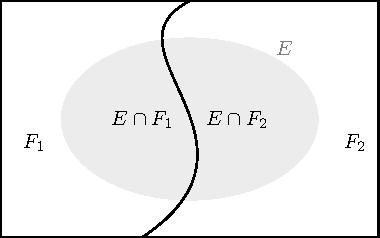
\includegraphics{ds4psy_files/figure-latex/unnamed-chunk-31-1} \end{center}

\end{exercise}

\hypertarget{posterior-predictive-checks}{%
\section{Posterior predictive checks}\label{posterior-predictive-checks}}

La distribuzione predittiva a posteriori viene utilizzata per eseguire i cosiddetti \emph{controlli predittivi a posteriori} (\emph{Posterior Predictive Checks}, PPC). Ricordiamo che la distribuzione predittiva a posteriori corrisponde alla simulazione di un campione di dati generati utilizzando le proprietà del modello adattato. Nei PPC si realizza un confronto grafico tra \(p(y^{rep} \mid y)\) e i dati osservati \(y\). Confrontando visivamente gli aspetti chiave dei dati previsti futuri \(y^{rep}\) e dei dati osservati \(y\) possiamo determinare se il modello è adeguato.

Oltre al confronto tra le distribuzioni \(p(y)\) e \(p(y^{rep})\) è anche possibile un confronto tra la distribuzione di varie statistiche descrittive, i cui valori sono calcolati su diversi campioni \(y^{rep}\), e le corrispondenti statistiche descrittive calcolate sui dati osservati. Vengono solitamente considerate statistiche descrittive quali la media, la varianza, la deviazione standard, il minimo o il massimo. Ma confronti di questo tipo sono possibili per qualunque statistica descrittiva. Questi confronti sono chiamati PPC.

\begin{exercise}
Esaminiamo ora un set di dati che non seguono la distribuzione normale \citep{gelman2020regression}. I dati corrispondono ad una serie di misurazioni prese da Simon Newcomb nel 1882 come parte di un esperimento per stimare la velocità della luce. A questi dati verrà (inappropriatamente) adattata una distribuzione normale. L'obiettivo dell'esempio è quello di mostrare come i PPC possono rivelare la mancanza di adattamento di un modello ai dati.

I PPC mostrano che il modo più semplice per verificare l'adattamento del modello è quello di visualizzare \(y^{rep}\) insieme ai dati effettivi. Iniziamo a caricare i dati:

\begin{Shaded}
\begin{Highlighting}[]
\FunctionTok{library}\NormalTok{(}\StringTok{"MASS"}\NormalTok{)}
\FunctionTok{data}\NormalTok{(}\StringTok{"newcomb"}\NormalTok{)}
\end{Highlighting}
\end{Shaded}

Visualizziamo la distribuzione dei dati con un istogramma:

\begin{Shaded}
\begin{Highlighting}[]
\FunctionTok{tibble}\NormalTok{(newcomb) }\SpecialCharTok{\%\textgreater{}\%}
  \FunctionTok{ggplot}\NormalTok{(}\FunctionTok{aes}\NormalTok{(}\AttributeTok{x =}\NormalTok{ newcomb, }\FunctionTok{after\_stat}\NormalTok{(density))) }\SpecialCharTok{+}
  \FunctionTok{geom\_histogram}\NormalTok{(}\AttributeTok{binwidth =} \DecValTok{1}\NormalTok{)}
\end{Highlighting}
\end{Shaded}

\begin{center}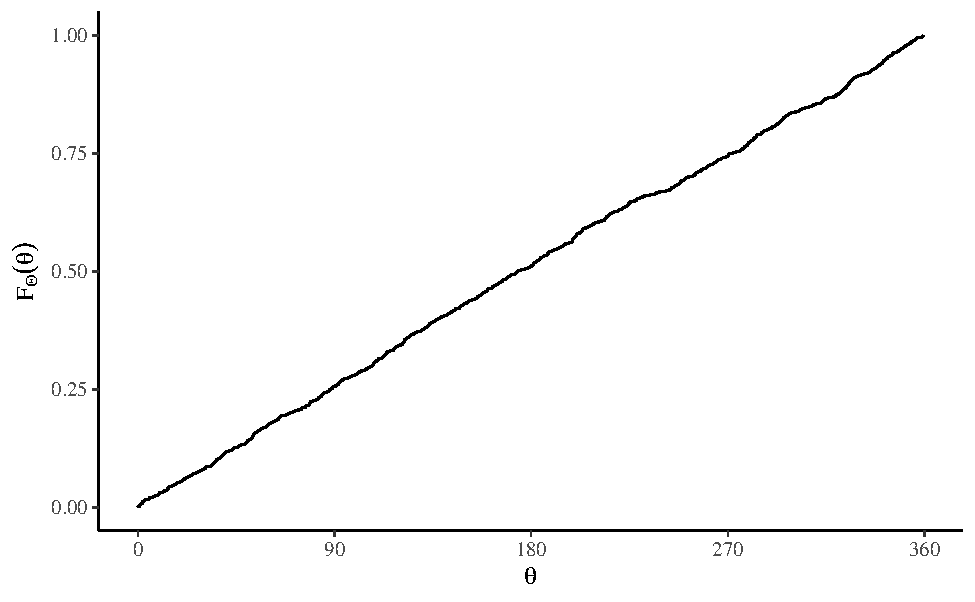
\includegraphics{ds4psy_files/figure-latex/unnamed-chunk-33-1} \end{center}

Creiamo un oggetto di tipo \texttt{list} dove inserire i dati:

\begin{Shaded}
\begin{Highlighting}[]
\NormalTok{data\_list }\OtherTok{\textless{}{-}} \FunctionTok{list}\NormalTok{(}
  \AttributeTok{y =}\NormalTok{ newcomb,}
  \AttributeTok{N =} \FunctionTok{length}\NormalTok{(newcomb)}
\NormalTok{)}
\end{Highlighting}
\end{Shaded}

Il codice Stan per il modello normale è il seguente:

\begin{Shaded}
\begin{Highlighting}[]
\NormalTok{modelString }\OtherTok{\textless{}{-}} \StringTok{"}
\StringTok{data \{}
\StringTok{  int\textless{}lower=0\textgreater{} N;}
\StringTok{  vector[N] y;}
\StringTok{\}}
\StringTok{parameters \{}
\StringTok{  real mu;}
\StringTok{  real\textless{}lower=0\textgreater{} sigma;}
\StringTok{\}}
\StringTok{model \{}
\StringTok{  mu \textasciitilde{} normal(25, 10);}
\StringTok{  sigma \textasciitilde{} cauchy(0, 10);}
\StringTok{  y \textasciitilde{} normal(mu, sigma);}
\StringTok{\}}
\StringTok{generated quantities \{}
\StringTok{  vector[N] y\_rep;}
\StringTok{  for (n in 1:N) \{}
\StringTok{    y\_rep[n] = normal\_rng(mu, sigma);}
\StringTok{  \}}
\StringTok{\}}
\StringTok{"}
\FunctionTok{writeLines}\NormalTok{(modelString, }\AttributeTok{con =} \StringTok{"code/newcomb.stan"}\NormalTok{)}
\end{Highlighting}
\end{Shaded}

Adattando il modello ai dati

\begin{Shaded}
\begin{Highlighting}[]
\NormalTok{file }\OtherTok{\textless{}{-}} \FunctionTok{file.path}\NormalTok{(}\StringTok{"code"}\NormalTok{, }\StringTok{"newcomb.stan"}\NormalTok{)}
\NormalTok{mod }\OtherTok{\textless{}{-}} \FunctionTok{cmdstan\_model}\NormalTok{(file)}
\NormalTok{fit }\OtherTok{\textless{}{-}}\NormalTok{ mod}\SpecialCharTok{$}\FunctionTok{sample}\NormalTok{(}
  \AttributeTok{data =}\NormalTok{ data\_list,}
  \AttributeTok{iter\_sampling =}\NormalTok{ 4000L,}
  \AttributeTok{iter\_warmup =}\NormalTok{ 2000L,}
  \AttributeTok{seed =}\NormalTok{ SEED,}
  \AttributeTok{chains =}\NormalTok{ 4L,}
  \AttributeTok{cores =}\NormalTok{ 4L,}
  \AttributeTok{refresh =} \DecValTok{0}\NormalTok{,}
  \AttributeTok{thin =} \DecValTok{1}
\NormalTok{)}
\end{Highlighting}
\end{Shaded}

otteniamo le seguenti stime dei parametri \(\mu\) e \(\sigma\):

\begin{Shaded}
\begin{Highlighting}[]
\NormalTok{fit}\SpecialCharTok{$}\FunctionTok{summary}\NormalTok{(}\FunctionTok{c}\NormalTok{(}\StringTok{"mu"}\NormalTok{, }\StringTok{"sigma"}\NormalTok{))}
\CommentTok{\#\textgreater{} \# A tibble: 2 x 10}
\CommentTok{\#\textgreater{}   variable  mean median    sd   mad    q5   q95  rhat}
\CommentTok{\#\textgreater{}   \textless{}chr\textgreater{}    \textless{}dbl\textgreater{}  \textless{}dbl\textgreater{} \textless{}dbl\textgreater{} \textless{}dbl\textgreater{} \textless{}dbl\textgreater{} \textless{}dbl\textgreater{} \textless{}dbl\textgreater{}}
\CommentTok{\#\textgreater{} 1 mu        26.2   26.2 1.33  1.30  24.0   28.4  1.00}
\CommentTok{\#\textgreater{} 2 sigma     10.9   10.8 0.958 0.943  9.40  12.5  1.00}
\CommentTok{\#\textgreater{} \# ... with 2 more variables: ess\_bulk \textless{}dbl\textgreater{},}
\CommentTok{\#\textgreater{} \#   ess\_tail \textless{}dbl\textgreater{}}
\end{Highlighting}
\end{Shaded}

Trasformiamo \texttt{fit} in un oggetto \texttt{stanfit}:

\begin{Shaded}
\begin{Highlighting}[]
\NormalTok{stanfit }\OtherTok{\textless{}{-}}\NormalTok{ rstan}\SpecialCharTok{::}\FunctionTok{read\_stan\_csv}\NormalTok{(fit}\SpecialCharTok{$}\FunctionTok{output\_files}\NormalTok{())}
\end{Highlighting}
\end{Shaded}

La distribuzione a posteriori di \(\mu\) è

\begin{Shaded}
\begin{Highlighting}[]
\NormalTok{mu\_draws }\OtherTok{\textless{}{-}} \FunctionTok{as.matrix}\NormalTok{(stanfit, }\AttributeTok{pars =} \StringTok{"mu"}\NormalTok{)}
\FunctionTok{mcmc\_areas}\NormalTok{(mu\_draws, }\AttributeTok{prob =} \FloatTok{0.95}\NormalTok{) }\CommentTok{\# color 95\% interval}
\end{Highlighting}
\end{Shaded}

\begin{center}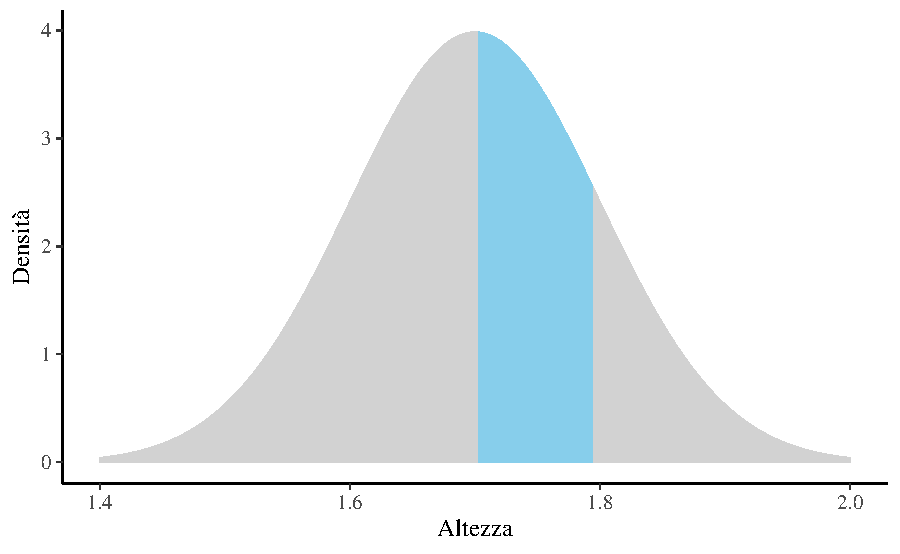
\includegraphics{ds4psy_files/figure-latex/unnamed-chunk-39-1} \end{center}

Confrontiamo \(\mu\) con la media di \(y\):

\begin{Shaded}
\begin{Highlighting}[]
\FunctionTok{mean}\NormalTok{(newcomb)}
\CommentTok{\#\textgreater{} [1] 26.21}
\end{Highlighting}
\end{Shaded}

Anche se trova la media giusta, il modello non è comunque adeguato a prevedere le altre proprietà della \(y\). Estraiamo \(y^{rep}\) dall'oggetto \texttt{stanfit}:

\begin{Shaded}
\begin{Highlighting}[]
\NormalTok{y\_rep }\OtherTok{\textless{}{-}} \FunctionTok{as.matrix}\NormalTok{(stanfit, }\AttributeTok{pars =} \StringTok{"y\_rep"}\NormalTok{)}
\FunctionTok{dim}\NormalTok{(y\_rep)}
\CommentTok{\#\textgreater{} [1] 16000    66}
\end{Highlighting}
\end{Shaded}

I valori \texttt{y\_rep} sono i dati della distribuzione predittiva a posteriori che sono stati simulati usando gli stessi valori \(X\) dei predittori utilizzati per adattare il modello. Il confronto tra l'istogramma della \(y\) e gli istogrammi di diversi campioni \(y^{rep}\) mostra una scarsa corrispondenza tra i due:

\begin{Shaded}
\begin{Highlighting}[]
\FunctionTok{ppc\_hist}\NormalTok{(data\_list}\SpecialCharTok{$}\NormalTok{y, y\_rep[}\DecValTok{1}\SpecialCharTok{:}\DecValTok{8}\NormalTok{, ], }\AttributeTok{binwidth =} \DecValTok{1}\NormalTok{)}
\end{Highlighting}
\end{Shaded}

\begin{center}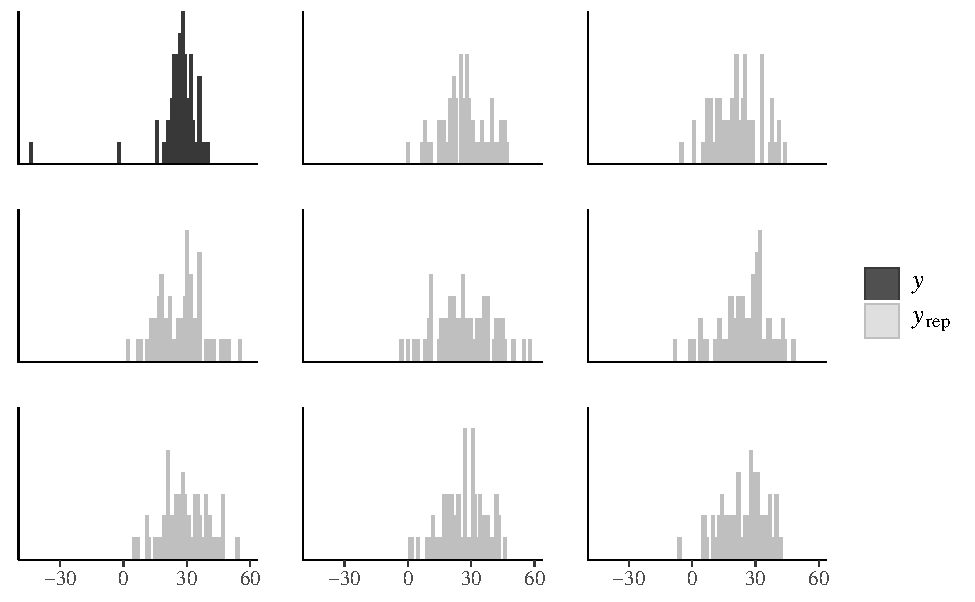
\includegraphics{ds4psy_files/figure-latex/unnamed-chunk-42-1} \end{center}

Alla stessa conclusione si giunge tramite un confronto tra la funzione di densità empirica della \(y\) e quella di diversi campioni \(y^{rep}\):

\begin{Shaded}
\begin{Highlighting}[]
\FunctionTok{ppc\_dens\_overlay}\NormalTok{(data\_list}\SpecialCharTok{$}\NormalTok{y, y\_rep[}\DecValTok{1}\SpecialCharTok{:}\DecValTok{50}\NormalTok{, ])}
\end{Highlighting}
\end{Shaded}

\begin{center}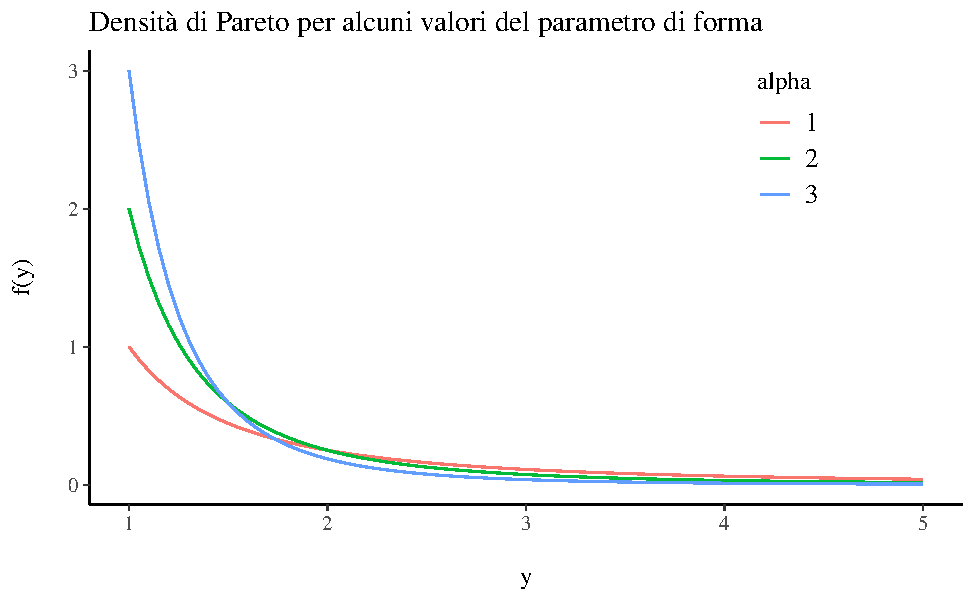
\includegraphics{ds4psy_files/figure-latex/unnamed-chunk-43-1} \end{center}

Generiamo ora i PPC per la media e il minimo della distribuzione:

\begin{Shaded}
\begin{Highlighting}[]
\FunctionTok{ppc\_stat\_2d}\NormalTok{(data\_list}\SpecialCharTok{$}\NormalTok{y, y\_rep, }\AttributeTok{stat =} \FunctionTok{c}\NormalTok{(}\StringTok{"mean"}\NormalTok{, }\StringTok{"min"}\NormalTok{))}
\end{Highlighting}
\end{Shaded}

\begin{center}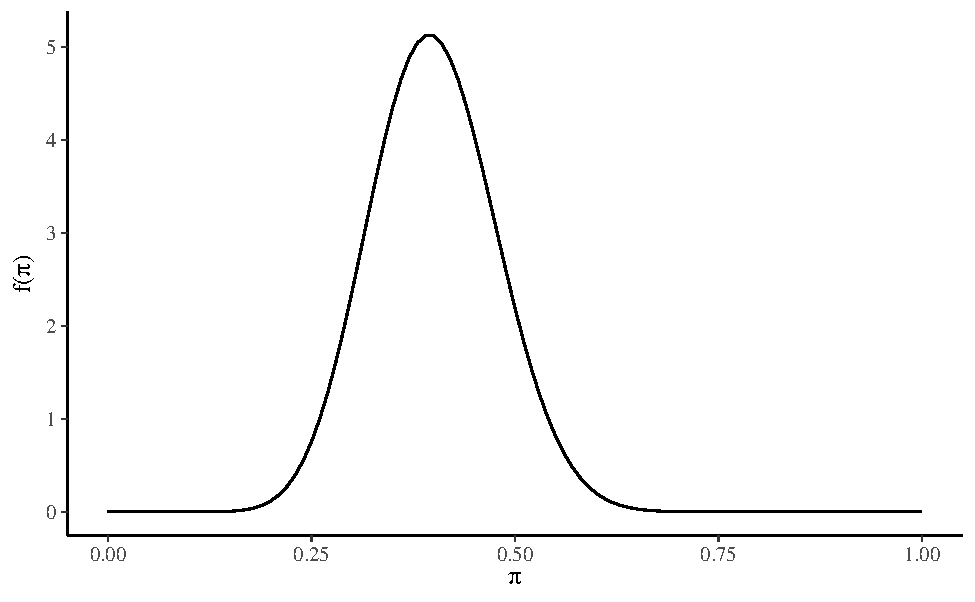
\includegraphics{ds4psy_files/figure-latex/unnamed-chunk-44-1} \end{center}

Mentre la media viene riprodotta accuratamente dal modello (come abbiamo visto sopra), ciò non è vero per il minimo dela distribuzione. L'origine di questa mancanza di adattamento è il fatto che la distribuzione delle misurazioni della velocità della luce è asimmetrica negativa. Dato che ci sono poche osservazioni nella coda negativa della distribuzione, solo per fare un esempio, utilizzeremo ora un secondo modello che ipotizza una distribuzione \(t\) di Student:

\begin{Shaded}
\begin{Highlighting}[]
\NormalTok{modelString }\OtherTok{=} \StringTok{"}
\StringTok{data \{}
\StringTok{  int\textless{}lower=0\textgreater{} N;}
\StringTok{  vector[N] y;}
\StringTok{\}}
\StringTok{parameters \{}
\StringTok{  real mu;}
\StringTok{  real\textless{}lower=0\textgreater{} sigma;}
\StringTok{  real\textless{}lower=0\textgreater{} nu;}
\StringTok{\}}
\StringTok{model \{}
\StringTok{  mu \textasciitilde{} normal(25, 10);}
\StringTok{  sigma \textasciitilde{} cauchy(0, 10);}
\StringTok{  nu \textasciitilde{} cauchy(0, 10);}
\StringTok{  y \textasciitilde{} student\_t(nu, mu, sigma);}
\StringTok{\}}
\StringTok{generated quantities \{}
\StringTok{  vector[N] y\_rep;}
\StringTok{  for (n in 1:N) \{}
\StringTok{    y\_rep[n] = student\_t\_rng(nu, mu, sigma);}
\StringTok{  \}}
\StringTok{\}}
\StringTok{"}
\FunctionTok{writeLines}\NormalTok{(modelString, }\AttributeTok{con =} \StringTok{"code/newcomb2.stan"}\NormalTok{)}
\end{Highlighting}
\end{Shaded}

Adattiamo questo secondo modello ai dati.

\begin{Shaded}
\begin{Highlighting}[]
\NormalTok{file }\OtherTok{\textless{}{-}} \FunctionTok{file.path}\NormalTok{(}\StringTok{"code"}\NormalTok{, }\StringTok{"newcomb2.stan"}\NormalTok{)}
\NormalTok{mod }\OtherTok{\textless{}{-}} \FunctionTok{cmdstan\_model}\NormalTok{(file)}
\NormalTok{fit }\OtherTok{\textless{}{-}}\NormalTok{ mod}\SpecialCharTok{$}\FunctionTok{sample}\NormalTok{(}
  \AttributeTok{data =}\NormalTok{ data\_list,}
  \AttributeTok{iter\_sampling =}\NormalTok{ 4000L,}
  \AttributeTok{iter\_warmup =}\NormalTok{ 2000L,}
  \AttributeTok{seed =}\NormalTok{ SEED,}
  \AttributeTok{chains =}\NormalTok{ 4L,}
  \AttributeTok{cores =}\NormalTok{ 4L,}
  \AttributeTok{parallel\_chains =}\NormalTok{ 2L,}
  \AttributeTok{refresh =} \DecValTok{0}\NormalTok{,}
  \AttributeTok{thin =} \DecValTok{1}
\NormalTok{)}
\CommentTok{\#\textgreater{} Running MCMC with 4 parallel chains...}
\CommentTok{\#\textgreater{} }
\CommentTok{\#\textgreater{} Chain 1 finished in 0.3 seconds.}
\CommentTok{\#\textgreater{} Chain 2 finished in 0.3 seconds.}
\CommentTok{\#\textgreater{} Chain 3 finished in 0.3 seconds.}
\CommentTok{\#\textgreater{} Chain 4 finished in 0.3 seconds.}
\CommentTok{\#\textgreater{} }
\CommentTok{\#\textgreater{} All 4 chains finished successfully.}
\CommentTok{\#\textgreater{} Mean chain execution time: 0.3 seconds.}
\CommentTok{\#\textgreater{} Total execution time: 0.5 seconds.}
\end{Highlighting}
\end{Shaded}

Per questo secondo modello il confronto tra la funzione di densità empirica della \(y\) e quella di diversi campioni \(y^{rep}\) risulta adeguato:

\begin{Shaded}
\begin{Highlighting}[]
\NormalTok{stanfit }\OtherTok{\textless{}{-}}\NormalTok{ rstan}\SpecialCharTok{::}\FunctionTok{read\_stan\_csv}\NormalTok{(fit}\SpecialCharTok{$}\FunctionTok{output\_files}\NormalTok{())}
\NormalTok{y\_rep }\OtherTok{\textless{}{-}} \FunctionTok{as.matrix}\NormalTok{(stanfit, }\AttributeTok{pars =} \StringTok{"y\_rep"}\NormalTok{)}
\FunctionTok{ppc\_dens\_overlay}\NormalTok{(data\_list}\SpecialCharTok{$}\NormalTok{y, y\_rep[}\DecValTok{1}\SpecialCharTok{:}\DecValTok{50}\NormalTok{, ])}
\end{Highlighting}
\end{Shaded}

\begin{center}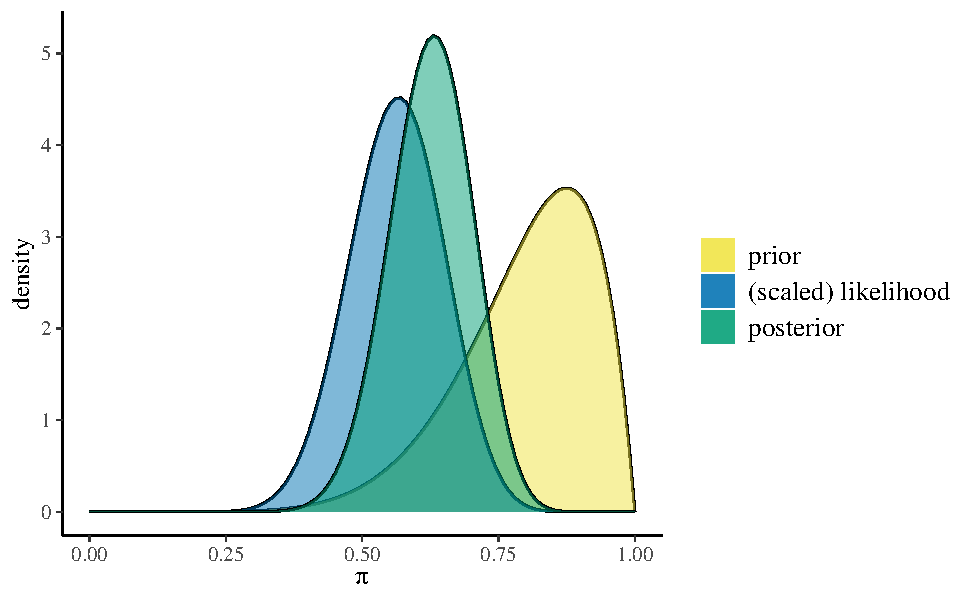
\includegraphics{ds4psy_files/figure-latex/unnamed-chunk-47-1} \end{center}

Inoltre, anche la statistica ``minimo della distribuzione'' viene ben predetta dal modello.

\begin{Shaded}
\begin{Highlighting}[]
\FunctionTok{ppc\_stat\_2d}\NormalTok{(data\_list}\SpecialCharTok{$}\NormalTok{y, y\_rep, }\AttributeTok{stat =} \FunctionTok{c}\NormalTok{(}\StringTok{"mean"}\NormalTok{, }\StringTok{"min"}\NormalTok{))}
\end{Highlighting}
\end{Shaded}

\begin{center}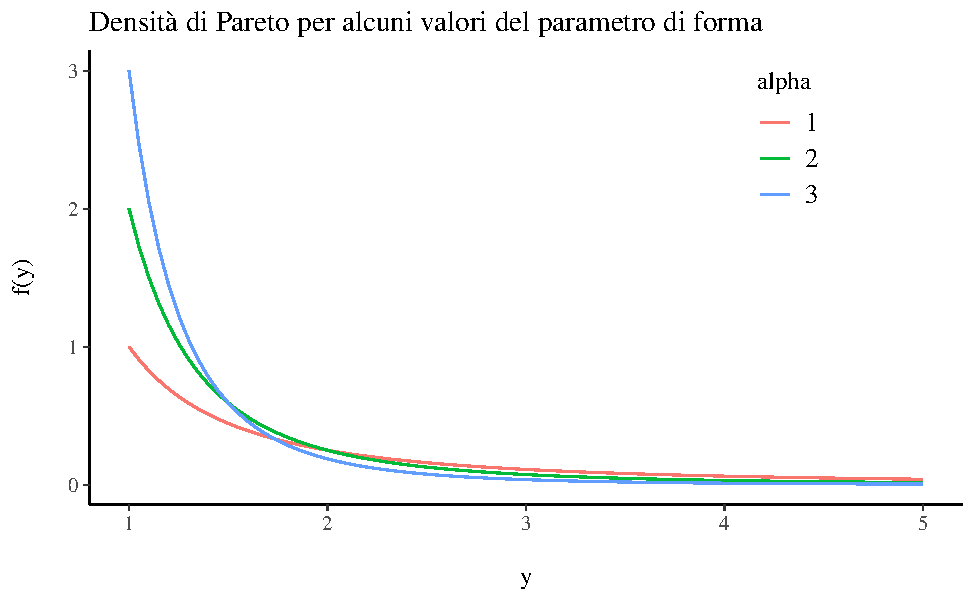
\includegraphics{ds4psy_files/figure-latex/unnamed-chunk-48-1} \end{center}

In conclusione, per le misurazioni della velocità della luce di Newcomb l'accuratezza predittiva del modello basato sulla distribuzione \(t\) di Student è chiaramente migliore di quella del modello normale.
\end{exercise}

\hypertarget{considerazioni-conclusive-1}{%
\section*{Considerazioni conclusive}\label{considerazioni-conclusive-1}}


Questo capitolo presenta i controlli predittivi a posteriori. A questo proposito è necessario notare un punto importante: i controlli predittivi a posteriori, quando suggeriscono un buon adattamento del modello alle caratterische dei dati previsti futuri \(y^{rep}\), non forniscono necessariamente una forte evidenza della capacità del modello di generalizzarsi a nuovi campioni di dati. Una tale evidenza sulla generalizzabilità del modello può solo essere fornita da studi di \emph{holdout validation}, ovvero da studi nei quali viene utilizzato un \emph{nuovo} campione di dati. Se i PPC mostrano un cattivo adattamento del modello ai dati previsti futuri, però, questo controllo fornisce una forte evidenza di una errata specificazione del modello.

\hypertarget{normal-normal-mod-stan}{%
\chapter{Modello Normale-Normale}\label{normal-normal-mod-stan}}

\hypertarget{distribuzione-normale-normale-con-varianza-nota}{%
\section{Distribuzione Normale-Normale con varianza nota}\label{distribuzione-normale-normale-con-varianza-nota}}

Per \(\sigma^2\) nota, la v.c. gaussiana è distribuzione a priori coniugata della v.c. gaussiana. Siano \(Y_1, \dots, Y_n\) \(n\) variabili casuali i.i.d. che seguono la distribuzione gaussiana:

\[
Y_1, \dots, Y_n  \stackrel{iid}{\sim} \mathcal{N}(\mu, \sigma).
\]

Si vuole stimare \(\mu\) sulla base di \(n\) osservazioni \(y_1, \dots, y_n\). Considereremo qui solamente il caso in cui \(\sigma^2\) sia supposta perfettamente nota.

Ricordiamo che la densità di una gaussiana è

\[
p(y_i \mid \mu, \sigma) = \frac{1}{{\sigma \sqrt {2\pi}}}\exp\left\{{-\frac{(y_i - \mu)^2}{2\sigma^2}}\right\}.
\]

Essendo le variabili i.i.d., possiamo scrivere la densità congiunta come il prodotto delle singole densità e quindi si ottiene

\[
p(y \mid \mu) = \, \prod_{i=1}^n p(y_i \mid \mu).
\]

Una volta osservati i dati \(y\), la verosimiglianza diventa

\begin{align}
\mathcal{L}(\mu \mid y) =& \, \prod_{i=1}^n p(y_i \mid \mu) = \notag\\
& \frac{1}{{\sigma \sqrt {2\pi}}}\exp\left\{{-\frac{(y_1 - \mu)^2}{2\sigma^2}}\right\} \times \notag\\
 & \frac{1}{{\sigma \sqrt {2\pi}}}\exp\left\{{-\frac{(y_2 - \mu)^2}{2\sigma^2}}\right\} \times  \notag\\
& \vdots \notag\\
 & \frac{1}{{\sigma \sqrt {2\pi}}}\exp\left\{{-\frac{(y_n - \mu)^2}{2\sigma^2}}\right\}.
\end{align}

Se viene scelta una densità a priori gaussiana, ciò fa sì che anche la densità a posteriori sia gaussiana. Supponiamo che

\begin{equation}
p(\mu) = \frac{1}{{\tau_0 \sqrt {2\pi}}}\exp\left\{{-\frac{(\mu - \mu_0)^2}{2\tau_0^2}}\right\},
\label{eq:prior-mu-norm-norm}
\end{equation}

ovvero che la distribuzione a priori di \(\mu\) sia gaussiana con media \(\mu_0\) e varianza \(\tau_0^2\). Possiamo dire che \(\mu_0\) rappresenta il valore ritenuto più probabile per \(\mu\) e \(\tau_0^2\) il grado di incertezza che abbiamo rispetto a tale valore.

Svolgendo una serie di passaggi algebrici, si arriva a

\begin{equation}
p(\mu \mid y) = \frac{1}{{\tau_p \sqrt {2\pi}}}\exp\left\{{-\frac{(\mu - \mu_p)^2}{2\tau_p^2}}\right\},
\label{eq:post-norm-norm}
\end{equation}

dove

\begin{equation}
\mu_p = \frac{\frac{1}{\tau_0^2}\mu_0+ \frac{n}{\sigma^2}\bar{y}}{\frac {1}{\tau_0^2} + \frac{n}{\sigma^2}} 
\label{eq:post-norm-mup}
\end{equation}

e

\begin{equation}
\tau_p^2 = \frac{1}{\frac {1}{\tau_0^2}+ \frac{n}{\sigma^2}}.
\label{eq:post-norm-taup2}
\end{equation}

In altri termini, se la distribuzione a priori per \(\mu\) è gaussiana, la distribuzione a posteriori è anch'essa gaussiana con valore atteso (a posteriori) \(\mu_p\) e varianza (a posteriori) \(\tau_p^2\) date dalle espressioni precedenti.

In conclusione, il risultato trovato indica che:

\begin{itemize}
\tightlist
\item
  il valore atteso a posteriori è una media pesata fra il valore atteso a priori \(\mu_0\) e la media campionaria \(\bar{y}\); il peso della media campionaria è tanto maggiore tanto più è grande \(n\) (il numero di osservazioni) e \(\tau_0^2\) (l'incertezza iniziale);
\item
  l'incertezza (varianza) a posteriori \(\tau_p^2\) è sempre più piccola dell'incertezza a priori \(\tau_0^2\) e diminuisce al crescere di \(n\).
\end{itemize}

\hypertarget{il-modello-normale-con-stan}{%
\section{Il modello Normale con Stan}\label{il-modello-normale-con-stan}}

Per esaminare un esempio pratico, consideriamo i 30 valori BDI-II dei soggetti clinici di \citet{zetschefuture2019}:

\begin{Shaded}
\begin{Highlighting}[]
\NormalTok{df }\OtherTok{\textless{}{-}} \FunctionTok{data.frame}\NormalTok{(}
  \AttributeTok{y =} \FunctionTok{c}\NormalTok{(}
    \FloatTok{26.0}\NormalTok{, }\FloatTok{35.0}\NormalTok{, }\DecValTok{30}\NormalTok{, }\DecValTok{25}\NormalTok{, }\DecValTok{44}\NormalTok{, }\DecValTok{30}\NormalTok{, }\DecValTok{33}\NormalTok{, }\DecValTok{43}\NormalTok{, }\DecValTok{22}\NormalTok{, }\DecValTok{43}\NormalTok{,}
    \DecValTok{24}\NormalTok{, }\DecValTok{19}\NormalTok{, }\DecValTok{39}\NormalTok{, }\DecValTok{31}\NormalTok{, }\DecValTok{25}\NormalTok{, }\DecValTok{28}\NormalTok{, }\DecValTok{35}\NormalTok{, }\DecValTok{30}\NormalTok{, }\DecValTok{26}\NormalTok{, }\DecValTok{31}\NormalTok{, }\DecValTok{41}\NormalTok{,}
    \DecValTok{36}\NormalTok{, }\DecValTok{26}\NormalTok{, }\DecValTok{35}\NormalTok{, }\DecValTok{33}\NormalTok{, }\DecValTok{28}\NormalTok{, }\DecValTok{27}\NormalTok{, }\DecValTok{34}\NormalTok{, }\DecValTok{27}\NormalTok{, }\DecValTok{22}
\NormalTok{  )}
\NormalTok{)}
\end{Highlighting}
\end{Shaded}

Calcoliamo le statistiche descrittive del campione di dati:

\begin{Shaded}
\begin{Highlighting}[]
\NormalTok{df }\SpecialCharTok{\%\textgreater{}\%} 
  \FunctionTok{summarise}\NormalTok{(}
    \AttributeTok{sample\_mean =} \FunctionTok{mean}\NormalTok{(y),}
    \AttributeTok{sample\_sd =} \FunctionTok{sd}\NormalTok{(y)}
\NormalTok{  )}
\CommentTok{\#\textgreater{}   sample\_mean sample\_sd}
\CommentTok{\#\textgreater{} 1       30.93     6.607}
\end{Highlighting}
\end{Shaded}

Nella discussione seguente assumeremo che \(\mu\) e \(\sigma\) siano indipendenti. Assegneremo a \(\mu\) una distribuzione a priori \(\mathcal{N}(25, 2)\) e a \(\sigma\) una distribuzione a priori \(Cauchy(0, 3)\).

Il modello statistico diventa:

\begin{align}
Y_i &\sim \mathcal{N}(\mu, \sigma) \notag\\
\mu &\sim \mathcal{N}(\mu_{\mu} = 25, \sigma_{\mu} = 2) \notag\\
\sigma &\sim \Cauchy(0, 3) \notag
\end{align}

In base al modello definito, la variabile casuale \(Y\) segue la distribuzione Normale di parametri \(\mu\) e \(\sigma\). Il parametro \(\mu\) è sconosciuto e abbiamo deciso di descrivere la nostra incertezza relativa ad esso mediante una distribuzione a priori Normale con media uguale a 25 e deviazione standard pari a 2. L'incertezza relativa a \(\sigma\) è quantificata da una distribuzione a priori half-Cauchy(0, 5), come indicato nella figura seguente:

\begin{Shaded}
\begin{Highlighting}[]
\FunctionTok{data.frame}\NormalTok{(}\AttributeTok{x =} \FunctionTok{c}\NormalTok{(}\DecValTok{0}\NormalTok{, }\DecValTok{20}\NormalTok{)) }\SpecialCharTok{\%\textgreater{}\%}
  \FunctionTok{ggplot}\NormalTok{(}\FunctionTok{aes}\NormalTok{(x)) }\SpecialCharTok{+}
  \FunctionTok{stat\_function}\NormalTok{(}
    \AttributeTok{fun =}\NormalTok{ dcauchy,}
    \AttributeTok{n =} \FloatTok{1e3}\NormalTok{,}
    \AttributeTok{args =} \FunctionTok{list}\NormalTok{(}\AttributeTok{location =} \DecValTok{0}\NormalTok{, }\AttributeTok{scale =} \DecValTok{3}\NormalTok{)}
\NormalTok{  ) }\SpecialCharTok{+}
  \FunctionTok{ylab}\NormalTok{(}\StringTok{"P(x)"}\NormalTok{) }\SpecialCharTok{+}
  \FunctionTok{theme}\NormalTok{(}\AttributeTok{legend.position =} \StringTok{"none"}\NormalTok{)}
\end{Highlighting}
\end{Shaded}

\begin{center}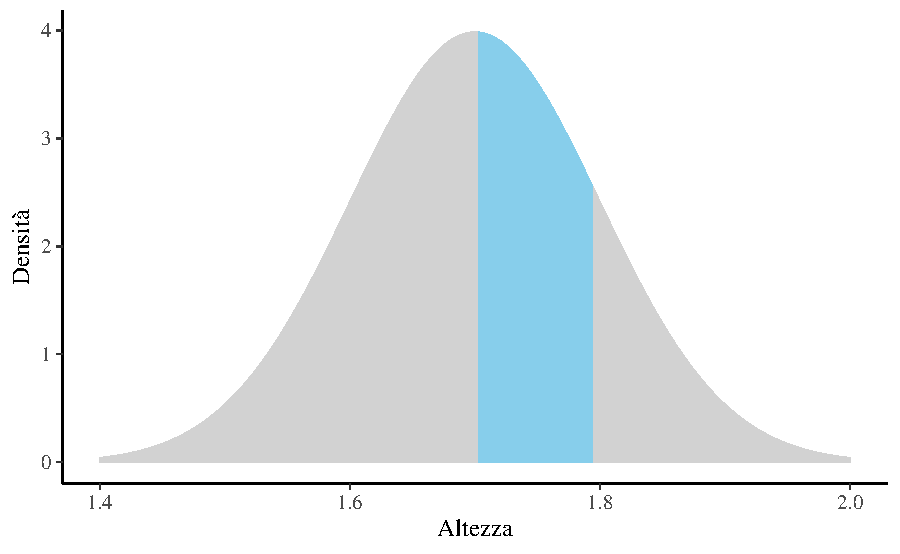
\includegraphics{ds4psy_files/figure-latex/unnamed-chunk-52-1} \end{center}

Dato che il modello è Normale-Normale, è possibile una soluzione analitica, come descritto in precedenza per il caso in cui \(\sigma\) è noto. In tali condizioni, la distribuzione a posteriori per \(\mu\) può essere trovata con la funzione \texttt{bayesrules:::summarize\_normal\_normal()}:

\begin{Shaded}
\begin{Highlighting}[]
\NormalTok{bayesrules}\SpecialCharTok{:::}\FunctionTok{summarize\_normal\_normal}\NormalTok{(}
  \AttributeTok{mean =} \DecValTok{25}\NormalTok{, }\AttributeTok{sd =} \DecValTok{2}\NormalTok{, }\AttributeTok{sigma =} \FunctionTok{sd}\NormalTok{(df}\SpecialCharTok{$}\NormalTok{y),}
  \AttributeTok{y\_bar =} \FunctionTok{mean}\NormalTok{(df}\SpecialCharTok{$}\NormalTok{y), }\AttributeTok{n =} \DecValTok{30}
\NormalTok{)}
\CommentTok{\#\textgreater{}       model  mean  mode   var    sd}
\CommentTok{\#\textgreater{} 1     prior 25.00 25.00 4.000 2.000}
\CommentTok{\#\textgreater{} 2 posterior 29.35 29.35 1.067 1.033}
\end{Highlighting}
\end{Shaded}

La rappresentazione grafica della funzione a priori, della verosimiglianza e della distribuzione a posteriori per \(\mu\) è fornita da:

\begin{Shaded}
\begin{Highlighting}[]
\NormalTok{bayesrules}\SpecialCharTok{:::}\FunctionTok{plot\_normal\_normal}\NormalTok{(}
  \AttributeTok{mean =} \DecValTok{25}\NormalTok{, }\AttributeTok{sd =} \DecValTok{2}\NormalTok{, }\AttributeTok{sigma =} \FunctionTok{sd}\NormalTok{(df}\SpecialCharTok{$}\NormalTok{y), }
  \AttributeTok{y\_bar =} \FunctionTok{mean}\NormalTok{(df}\SpecialCharTok{$}\NormalTok{y), }\AttributeTok{n =} \DecValTok{30}
\NormalTok{)}
\end{Highlighting}
\end{Shaded}

\begin{center}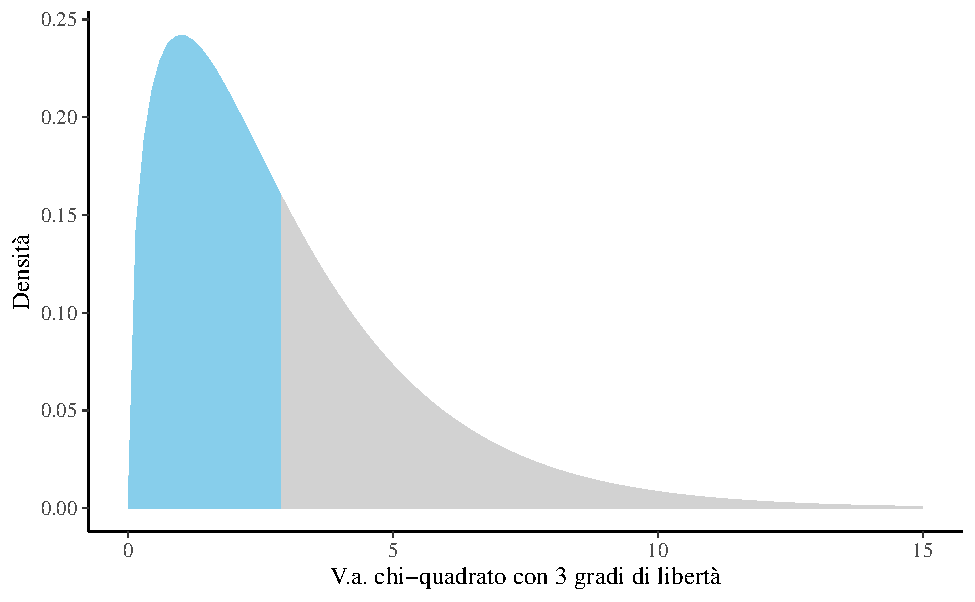
\includegraphics{ds4psy_files/figure-latex/unnamed-chunk-54-1} \end{center}

La procedura MCMC utilizzata da Stan è basata su un campionamento Monte Carlo Hamiltoniano che non richiede l'uso di distribuzioni a priori coniugate. Pertanto per i parametri è possibile scegliere una qualunque distribuzione a priori arbitraria.

Per continuare con l'esempio, poniamoci il problema di trovare le distribuzioni a posteriori dei parametri \(\mu\) e \(\sigma\) usando le funzioni del pacchetto \texttt{cmdstanr}. Il modello statistico descritto sopra si può scrivere in Stan nel modo seguente:

\begin{Shaded}
\begin{Highlighting}[]
\NormalTok{modelString }\OtherTok{=} \StringTok{"}
\StringTok{data \{}
\StringTok{  int\textless{}lower=0\textgreater{} N;}
\StringTok{  vector[N] y;}
\StringTok{\}}
\StringTok{parameters \{}
\StringTok{  real mu;}
\StringTok{  real\textless{}lower=0\textgreater{} sigma;}
\StringTok{\}}
\StringTok{model \{}
\StringTok{  mu \textasciitilde{} normal(25, 2);}
\StringTok{  sigma \textasciitilde{} cauchy(0, 3);}
\StringTok{  y \textasciitilde{} normal(mu, sigma);}
\StringTok{\}}
\StringTok{"}
\FunctionTok{writeLines}\NormalTok{(modelString, }\AttributeTok{con =} \StringTok{"code/normalmodel.stan"}\NormalTok{)}
\end{Highlighting}
\end{Shaded}

Si noti che, nel modello, il parametro \(\sigma\) è considerato incognito.

Sistemiamo i dati nel formato appropriato per potere essere letti da Stan:

\begin{Shaded}
\begin{Highlighting}[]
\NormalTok{data\_list }\OtherTok{\textless{}{-}} \FunctionTok{list}\NormalTok{(}
  \AttributeTok{N =} \FunctionTok{length}\NormalTok{(df}\SpecialCharTok{$}\NormalTok{y),}
  \AttributeTok{y =}\NormalTok{ df}\SpecialCharTok{$}\NormalTok{y}
\NormalTok{)}
\end{Highlighting}
\end{Shaded}

Leggiamo il file in cui abbiamo salvato il codice Stan

\begin{Shaded}
\begin{Highlighting}[]
\NormalTok{file }\OtherTok{\textless{}{-}} \FunctionTok{file.path}\NormalTok{(}\StringTok{"code"}\NormalTok{, }\StringTok{"normalmodel.stan"}\NormalTok{)}
\end{Highlighting}
\end{Shaded}

compiliamo il modello

\begin{Shaded}
\begin{Highlighting}[]
\NormalTok{mod }\OtherTok{\textless{}{-}} \FunctionTok{cmdstan\_model}\NormalTok{(file)}
\end{Highlighting}
\end{Shaded}

ed eseguiamo il campionamento MCMC:

\begin{Shaded}
\begin{Highlighting}[]
\NormalTok{fit }\OtherTok{\textless{}{-}}\NormalTok{ mod}\SpecialCharTok{$}\FunctionTok{sample}\NormalTok{(}
  \AttributeTok{data =}\NormalTok{ data\_list,}
  \AttributeTok{iter\_sampling =}\NormalTok{ 4000L,}
  \AttributeTok{iter\_warmup =}\NormalTok{ 2000L,}
  \AttributeTok{seed =}\NormalTok{ SEED,}
  \AttributeTok{chains =}\NormalTok{ 4L,}
  \AttributeTok{parallel\_chains =}\NormalTok{ 2L,}
  \AttributeTok{refresh =} \DecValTok{0}\NormalTok{,}
  \AttributeTok{thin =} \DecValTok{1}
\NormalTok{)}
\end{Highlighting}
\end{Shaded}

Le stime a posteriori dei parametri si ottengono con:

\begin{Shaded}
\begin{Highlighting}[]
\NormalTok{fit}\SpecialCharTok{$}\FunctionTok{summary}\NormalTok{(}\FunctionTok{c}\NormalTok{(}\StringTok{"mu"}\NormalTok{, }\StringTok{"sigma"}\NormalTok{))}
\CommentTok{\#\textgreater{} \# A tibble: 2 x 10}
\CommentTok{\#\textgreater{}   variable  mean median    sd   mad    q5   q95  rhat}
\CommentTok{\#\textgreater{}   \textless{}chr\textgreater{}    \textless{}dbl\textgreater{}  \textless{}dbl\textgreater{} \textless{}dbl\textgreater{} \textless{}dbl\textgreater{} \textless{}dbl\textgreater{} \textless{}dbl\textgreater{} \textless{}dbl\textgreater{}}
\CommentTok{\#\textgreater{} 1 mu       29.3   29.3  1.11  1.10  27.4  31.0   1.00}
\CommentTok{\#\textgreater{} 2 sigma     6.89   6.78 0.959 0.910  5.52  8.63  1.00}
\CommentTok{\#\textgreater{} \# ... with 2 more variables: ess\_bulk \textless{}dbl\textgreater{},}
\CommentTok{\#\textgreater{} \#   ess\_tail \textless{}dbl\textgreater{}}
\end{Highlighting}
\end{Shaded}

oppure, dopo avere trasformato l'oggetto \texttt{fit} nel formato \texttt{stanfit},

\begin{Shaded}
\begin{Highlighting}[]
\NormalTok{stanfit }\OtherTok{\textless{}{-}}\NormalTok{ rstan}\SpecialCharTok{::}\FunctionTok{read\_stan\_csv}\NormalTok{(fit}\SpecialCharTok{$}\FunctionTok{output\_files}\NormalTok{())}
\end{Highlighting}
\end{Shaded}

con

\begin{Shaded}
\begin{Highlighting}[]
\NormalTok{out }\OtherTok{\textless{}{-}}\NormalTok{ rstantools}\SpecialCharTok{::}\FunctionTok{posterior\_interval}\NormalTok{(}\FunctionTok{as.matrix}\NormalTok{(stanfit), }\AttributeTok{prob =} \FloatTok{0.95}\NormalTok{)}
\NormalTok{out}
\CommentTok{\#\textgreater{}          2.5\%   97.5\%}
\CommentTok{\#\textgreater{} mu     26.990  31.349}
\CommentTok{\#\textgreater{} sigma   5.321   9.079}
\CommentTok{\#\textgreater{} lp\_\_  {-}77.914 {-}74.276}
\end{Highlighting}
\end{Shaded}

Possiamo dunque concludere, con un grado di certezza soggettiva del 95\%, che siamo sicuri che la media della popolazione da cui abbiamo tratto i dati è compresa nell'intervallo {[}26.99, 31.35{]}.

\hypertarget{il-modello-normale-con-quap}{%
\section{\texorpdfstring{Il modello normale con \texttt{quap()}}{Il modello normale con quap()}}\label{il-modello-normale-con-quap}}

Ripetiamo l'analisi precedente usando le funzioni del pacchetto \texttt{rethinking} per trovare le distribuzioni a posteriori dei parametri \(\mu\) e \(\sigma\). Definiamo il modello statistico mediante la funzione \texttt{alist()}:

\begin{Shaded}
\begin{Highlighting}[]
\NormalTok{flist }\OtherTok{\textless{}{-}} \FunctionTok{alist}\NormalTok{(}
\NormalTok{  y }\SpecialCharTok{\textasciitilde{}} \FunctionTok{dnorm}\NormalTok{(mu, sigma), }
\NormalTok{  mu }\SpecialCharTok{\textasciitilde{}} \FunctionTok{dnorm}\NormalTok{(}\DecValTok{25}\NormalTok{, }\DecValTok{2}\NormalTok{),}
\NormalTok{  sigma }\SpecialCharTok{\textasciitilde{}} \FunctionTok{dcauchy}\NormalTok{(}\DecValTok{0}\NormalTok{, }\DecValTok{3}\NormalTok{)}
\NormalTok{)}
\end{Highlighting}
\end{Shaded}

Le precedenti istruzioni \texttt{R} specificano una variabile casuale \(Y\) che si distribuisce come una Normale di parametri \(\mu\) e \(\sigma\); questa è la verosimiglianza. La distribuzione a priori del parametro \(\mu\) è una Normale di media 25 e deviazione standard 2. La distribuzione a priori del parametro \(\sigma\) è una half-Cauchy di parametri \texttt{location} = 0 e \texttt{scale} = 3.

Usiamo la funzione \texttt{quap()} per ottenere l'approssimazione quadratica delle distribuzioni a posteriori di \(\mu\) e \(\sigma\):

\begin{Shaded}
\begin{Highlighting}[]
\FunctionTok{set.seed}\NormalTok{(}\DecValTok{123}\NormalTok{)}
\NormalTok{m }\OtherTok{\textless{}{-}} \FunctionTok{quap}\NormalTok{( }
\NormalTok{  flist,}
  \AttributeTok{data =}\NormalTok{ df }
\NormalTok{)}
\end{Highlighting}
\end{Shaded}

L'intervallo di credibilità al 95\% è dato dalla funzione \texttt{precis()}:

\begin{Shaded}
\begin{Highlighting}[]
\NormalTok{out }\OtherTok{\textless{}{-}} \FunctionTok{precis}\NormalTok{(m, }\AttributeTok{prob =} \FloatTok{0.95}\NormalTok{)}
\NormalTok{out}
\CommentTok{\#\textgreater{}         mean     sd  2.5\%  97.5\%}
\CommentTok{\#\textgreater{} mu    29.388 1.0633 27.30 31.472}
\CommentTok{\#\textgreater{} sigma  6.501 0.8473  4.84  8.162}
\end{Highlighting}
\end{Shaded}

I risultati sono simili a quelli trovati in precedenza.

\hypertarget{il-modello-normale-con-brmsbrm}{%
\section{\texorpdfstring{Il modello normale con \texttt{brms::brm()}}{Il modello normale con brms::brm()}}\label{il-modello-normale-con-brmsbrm}}

Stimiamo ora la distribuzione a posteriori di \(\mu\) usando la funzione \texttt{brms::brm()}. In questo caso non è necessario scrivere il modello in forma esplicita, come abbiamo fatto usando linguaggio Stan. La sintassi specifiata di seguito viene trasformata in maniera automatica nel linguaggio Stan prima di adattare il modello ai dati:

\begin{Shaded}
\begin{Highlighting}[]
\NormalTok{fit3 }\OtherTok{\textless{}{-}} \FunctionTok{brm}\NormalTok{(}
  \AttributeTok{data =}\NormalTok{ df, }
  \AttributeTok{family =} \FunctionTok{gaussian}\NormalTok{(),}
\NormalTok{  y }\SpecialCharTok{\textasciitilde{}} \DecValTok{1}\NormalTok{,}
  \AttributeTok{prior =} \FunctionTok{c}\NormalTok{(}
    \FunctionTok{prior}\NormalTok{(}\FunctionTok{normal}\NormalTok{(}\DecValTok{25}\NormalTok{, }\DecValTok{2}\NormalTok{), }\AttributeTok{class =}\NormalTok{ Intercept),}
    \FunctionTok{prior}\NormalTok{(}\FunctionTok{cauchy}\NormalTok{(}\DecValTok{0}\NormalTok{, }\DecValTok{3}\NormalTok{), }\AttributeTok{class =}\NormalTok{ sigma)}
\NormalTok{  ),}
  \AttributeTok{iter =} \DecValTok{4000}\NormalTok{, }
  \AttributeTok{refresh =} \DecValTok{0}\NormalTok{, }
  \AttributeTok{chains =} \DecValTok{4}\NormalTok{,}
  \AttributeTok{backend =} \StringTok{"cmdstanr"}
\NormalTok{)}
\CommentTok{\#\textgreater{} Running MCMC with 4 chains, at most 8 in parallel...}
\CommentTok{\#\textgreater{} }
\CommentTok{\#\textgreater{} Chain 1 finished in 0.1 seconds.}
\CommentTok{\#\textgreater{} Chain 2 finished in 0.1 seconds.}
\CommentTok{\#\textgreater{} Chain 3 finished in 0.1 seconds.}
\CommentTok{\#\textgreater{} Chain 4 finished in 0.1 seconds.}
\CommentTok{\#\textgreater{} }
\CommentTok{\#\textgreater{} All 4 chains finished successfully.}
\CommentTok{\#\textgreater{} Mean chain execution time: 0.1 seconds.}
\CommentTok{\#\textgreater{} Total execution time: 0.2 seconds.}
\end{Highlighting}
\end{Shaded}

I trace-plot si ottengono con l'istruzione seguente:

\begin{Shaded}
\begin{Highlighting}[]
\FunctionTok{plot}\NormalTok{(fit3)}
\end{Highlighting}
\end{Shaded}

\begin{center}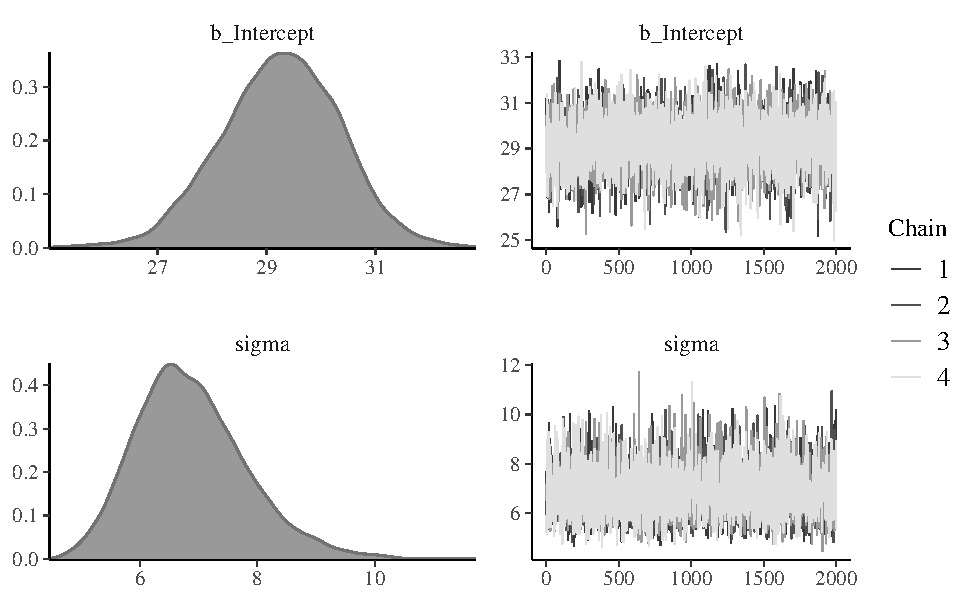
\includegraphics{ds4psy_files/figure-latex/unnamed-chunk-67-1} \end{center}

Le stime della distribuzione a posteriori si ottengono con la funzione \texttt{summary()}:

\begin{Shaded}
\begin{Highlighting}[]
\FunctionTok{summary}\NormalTok{(fit3)}
\CommentTok{\#\textgreater{}  Family: gaussian }
\CommentTok{\#\textgreater{}   Links: mu = identity; sigma = identity }
\CommentTok{\#\textgreater{} Formula: y \textasciitilde{} 1 }
\CommentTok{\#\textgreater{}    Data: df (Number of observations: 30) }
\CommentTok{\#\textgreater{}   Draws: 4 chains, each with iter = 2000; warmup = 0; thin = 1;}
\CommentTok{\#\textgreater{}          total post{-}warmup draws = 8000}
\CommentTok{\#\textgreater{} }
\CommentTok{\#\textgreater{} Population{-}Level Effects: }
\CommentTok{\#\textgreater{}           Estimate Est.Error l{-}95\% CI u{-}95\% CI Rhat}
\CommentTok{\#\textgreater{} Intercept    29.26      1.09    27.08    31.34 1.00}
\CommentTok{\#\textgreater{}           Bulk\_ESS Tail\_ESS}
\CommentTok{\#\textgreater{} Intercept     4559     4987}
\CommentTok{\#\textgreater{} }
\CommentTok{\#\textgreater{} Family Specific Parameters: }
\CommentTok{\#\textgreater{}       Estimate Est.Error l{-}95\% CI u{-}95\% CI Rhat}
\CommentTok{\#\textgreater{} sigma     6.88      0.94     5.27     9.01 1.00}
\CommentTok{\#\textgreater{}       Bulk\_ESS Tail\_ESS}
\CommentTok{\#\textgreater{} sigma     4366     4638}
\CommentTok{\#\textgreater{} }
\CommentTok{\#\textgreater{} Draws were sampled using sample(hmc). For each parameter, Bulk\_ESS}
\CommentTok{\#\textgreater{} and Tail\_ESS are effective sample size measures, and Rhat is the potential}
\CommentTok{\#\textgreater{} scale reduction factor on split chains (at convergence, Rhat = 1).}
\end{Highlighting}
\end{Shaded}

Nuovamente, i risultati sono molto simili a quelli ottenuti in precedenza.

\hypertarget{considerazioni-conclusive-2}{%
\section*{Considerazioni conclusive}\label{considerazioni-conclusive-2}}


Questo esempio ci mostra come calcolare l'intervallo di credibilità per la media di una v.c. Normale. La domanda più ovvia di analisi dei dati, dopo avere visto come creare l'intervallo di credibilità per la media di un gruppo, riguarda il confronto tra le medie di due gruppi. Questo però è un caso speciale di una tecnica di analisi dei dati più generale, chiamate analisi di regressione lineare. Prima di discutere il problema del confronto tra le medie di due gruppi è dunque necessario esaminare il modello statistico di regressione lineare.

\hypertarget{regr-models-intro}{%
\chapter{Introduzione al modello lineare}\label{regr-models-intro}}

Lo scopo della ricerca è trovare le associazioni tra le variabili e fare confronti fra le condizioni sperimentali. Nel caso della psicologia, il ricercatore vuole scoprire le leggi generali che descrivono le relazioni tra i costrutti psicologici e le relazioni che intercorrono tra i fenomeni psicologici e quelli non psicologici (sociali, economici, storici, \ldots). Abbiamo già visto come la correlazione di Pearson sia uno strumento adatto a questo scopo. Infatti, essa ci informa sulla direzione e sull'intensità della relazione lineare tra due variabili. Tuttavia, la correlazione non è sufficiente, in quanto il ricercatore ha a disposizione solo i dati di un campione, mentre vorrebbe descrivere la relazione tra le variabili nella popolazione. A causa della variabilità campionaria, le proprietà dei campioni sono necessariamente diverse da quelle della popolazione: ciò che si può osservare nella popolazione potrebbe non emergere nel campione e, al contrario, il campione manifesta caratteristiche che non sono necessariamente presenti nella popolazione. È dunque necessario chiarire, dal punto di vista statistico, il legame che intercorre tra le proprietà del campione e le proprietà della popolazione da cui esso è stato estratto. Il modello lineare utilizza la funzione matematica più semplice per descrivere la relazione fra due variabili, ovvero la funzione lineare. In questo Capitolo vedremo come si possa fare inferenza sulla relazione tra due variabili mediante il modello lineare bayesiano. Inizieremo a descrivere le proprietà geometriche della funzione lineare per poi utilizzare questa semplice funzione per costruire un modello statistico secondo un approccio bayesiano.

\hypertarget{la-funzione-lineare}{%
\section{La funzione lineare}\label{la-funzione-lineare}}

Iniziamo con un ripasso sulla funzione di lineare. Si chiama \emph{funzione lineare} una funzione del tipo

\begin{equation}
f(x) = a + b x,
\end{equation}

dove \(a\) e \(b\) sono delle costanti. Il grafico di tale funzione è una retta di cui il parametro \(b\) è detto \emph{coefficiente angolare} e il parametro \(a\) è detto \emph{intercetta} con l'asse delle \(y\) {[}infatti, la retta interseca l'asse \(y\) nel punto \((0,a)\), se \(b \neq 0\){]}.

Per assegnare un'interpretazione geometrica alle costanti \(a\) e \(b\) si consideri la funzione

\begin{equation}
y = b x.
\end{equation}

Tale funzione rappresenta un caso particolare, ovvero quello della \emph{proporzionalità diretta} tra \(x\) e \(y\). Il caso generale della linearità

\begin{equation}
y = a + b x
\end{equation}

non fa altro che sommare una costante \(a\) a ciascuno dei valori \(y = b x\). Nella funzione lineare \(y = a + b x\), se \(b\) è positivo allora \(y\) aumenta al crescere di \(x\); se \(b\) è negativo allora \(y\) diminuisce al crescere di \(x\); se \(b=0\) la retta è orizzontale, ovvero \(y\) non muta al variare di \(x\).

Consideriamo ora il coefficiente \(b\). Si consideri un punto \(x_0\) e un incremento arbitrario \(\varepsilon\) come indicato nella figura \ref{fig:linearfunction}. Le differenze \(\Delta x = (x_0 + \varepsilon) - x_0\) e \(\Delta y = f(x_0 + \varepsilon) - f(x_0)\) sono detti \emph{incrementi} di \(x\) e \(y\). Il coefficiente angolare \(b\) è uguale al rapporto

\begin{equation}
    b = \frac{\Delta y}{\Delta x} = \frac{f(x_0 + \varepsilon) - f(x_0)}{(x_0 + \varepsilon) - x_0},
\end{equation}

indipendentemente dalla grandezza degli incrementi \(\Delta x\) e \(\Delta y\). Il modo più semplice per assegnare un'interpretazione geometrica al coefficiente angolare (o pendenza) della retta è dunque quello di porre \(\Delta x = 1\). In tali circostanze infatti \(b = \Delta y\).

\begin{figure}[h]

{\centering 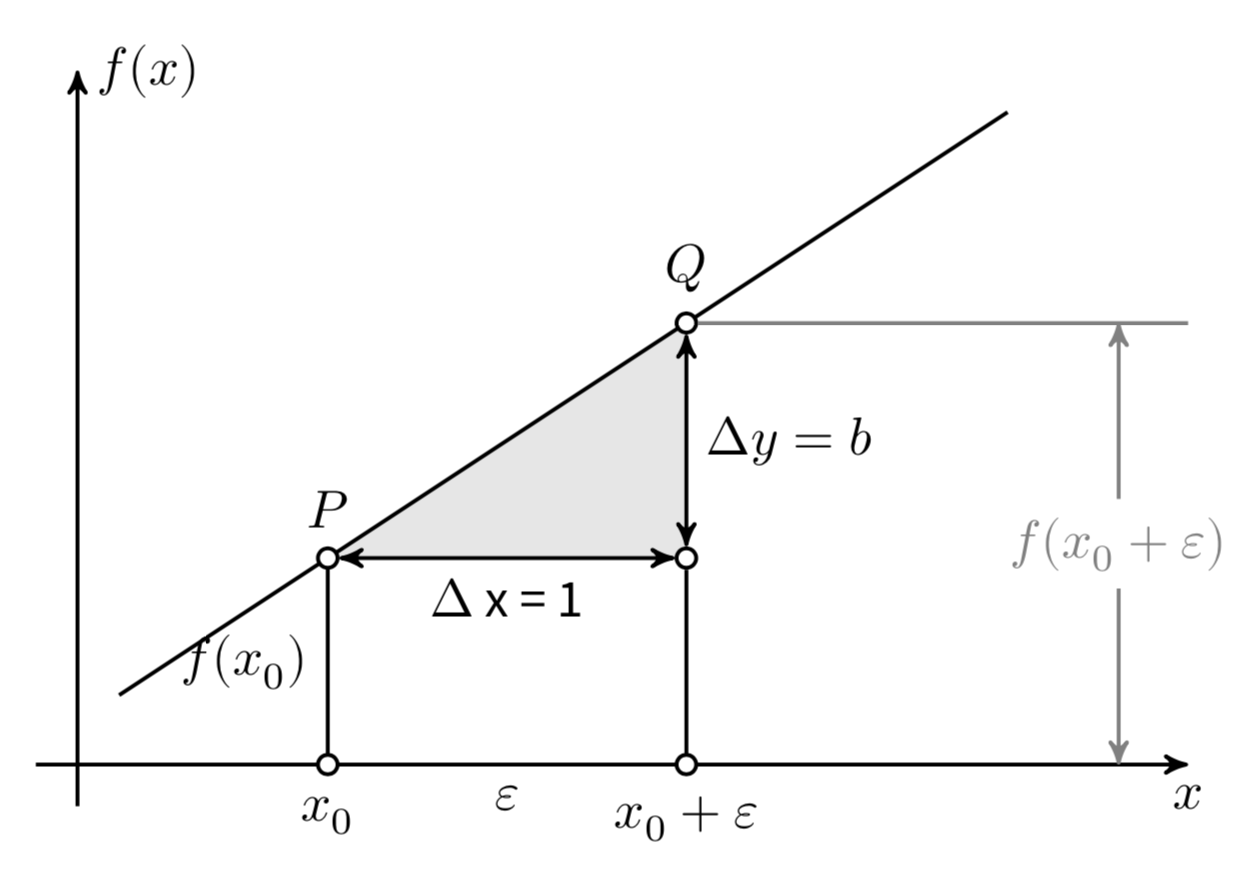
\includegraphics[width=4.17in]{images/linear_function} 

}

\caption{La funzione lineare $y = a + bx$.}\label{fig:linearfunction}
\end{figure}

\hypertarget{lerrore-di-misurazione}{%
\section{L'errore di misurazione}\label{lerrore-di-misurazione}}

Per descrivere l'associazione tra due variabili, tuttavia, la funzione lineare non è sufficiente. Nel mondo empirico, infatti, la relazione tra variabili non è mai perfettamente lineare. È dunque necessario includere nel modello lineare anche una componente d'errore, ovvero una componente della \(y\) che non può essere spiegata dal modello lineare. Nel caso di due sole variabili, questo ci conduce alla seguente formulazione del modello lineare:

\begin{equation}
y = \alpha + \beta x + \varepsilon,
\label{eq:regbivpop}
\end{equation}

laddove i parametri \(\alpha\) e \(\beta\) descrivono l'associazione tra le variabili casuali \(y\) e \(x\), e il termine d'errore \(\varepsilon\) specifica quant'è grande la porzione della variabile \(y\) che non può essere predetta nei termini di una relazione lineare con la \(x\).

Si noti che la \eqref{eq:regbivpop} consente di formulare una predizione, nei termini di un modello lineare, del valore atteso della \(y\) conoscendo \(x\), ovvero

\begin{equation}
\hat{y} = \mathbb{E}(y \mid x) = \alpha + \beta x.
\label{eq:regbivpop2}
\end{equation}

In altri termini, se i parametri del modello (\(\alpha\) e \(\beta\)) sono noti, allora è possibile predire la \(y\) sulla base della nostra conoscenza della \(x\). Per esempio, se conosciamo la relazione lineare tra quoziente di intelligenza ed aspettativa di vita, allora possiamo prevedere quanto a lungo vivrà una persona sulla base del suo QI. Sì, c'è una relazione lineare tra intelligenza e aspettativa di vita \citep{hambrick2015research}! Ma quando è accurata la previsione? Ciò dipende dal termine d'errore della \eqref{eq:regbivpop}. Il modello lineare fornisce un metodo per rispondere a domande di questo tipo\footnote{Per una discussione sugli aspetti di base del modello lineare, si veda il \href{https://openintro-ims.netlify.app/model-slr.html}{capitolo 7} di \emph{Introduction to Modern Statistics}.}.

\hypertarget{una-media-per-ciascuna-osservazione}{%
\section{Una media per ciascuna osservazione}\label{una-media-per-ciascuna-osservazione}}

In precedenza abbiamo visto come sia possibile stimare i parametri di un modello bayesiano Normale nel quale le osservazioni sono indipendenti e identicamente distribuite secondo una densità Normale,

\begin{equation}
Y_i \stackrel{i.i.d.}{\sim} \mathcal{N}(\mu, \sigma), \quad i = 1, \dots, n.
\label{eq:normalsamplingmodel}
\end{equation}

Il modello \eqref{eq:normalsamplingmodel} assume che ogni \(Y_i\) sia una realizzazione della stessa \(\mathcal{N}(\mu, \sigma^2)\). Da un punto di vista bayesiano\footnote{Per un'introduzione alla trattazione frequentista del modello lineare, si veda l'Appendice \ref{least-squares}.}, si assegnano distribuzioni a priori ai parametri \(\mu\) e \(\sigma\), si genera la verosimiglianza in base ai dati osservati e, con queste informazioni, si generano le distribuzione a posteriori dei parametri \citep{gelman2020regression}:

\begin{align}
Y_i \mid \mu, \sigma & \stackrel{iid}{\sim} \mathcal{N}(\mu, \sigma^2)\notag\\
\mu       & \sim \mathcal{N}(\mu_0, \tau^2) \notag\\
\sigma    & \sim \Cauchy(x_0, \gamma) \notag
\end{align}

È comune però che vengano però registrate altre variabili \(x_i\) che possono essere associate alla risposta di interesse \(y_i\). La variabile \(x_i\) viene chiamata \emph{predittore} (o variabile indipendente) in quanto il ricercatore è tipicamente interessato a predire il valore \(y_i\) a partire da \(x_i\). Come si può estende il modello Normale della \eqref{eq:normalsamplingmodel} per lo studio della possibile relazione tra \(y_i\) e \(x_i\)?

Il modello \eqref{eq:normalsamplingmodel} assume una media \(\mu\) comune per ciascuna osservazione \(Y_i\). Dal momento che desideriamo introdurre una nuova variabile \(x_i\) che assume un valore specifico per ciascuna osservazione \(y_i\), il modello \eqref{eq:normalsamplingmodel} può essere modificato in modo che la media comune \(\mu\) venga sostituita da una media \(\mu_i\) specifica a ciascuna \(i\)-esima osservazione:

\begin{equation}
Y_i \mid \mu_i, \sigma \stackrel{ind}{\sim} \mathcal{N}(\mu_i, \sigma), \quad i = 1, \dots, n.
\label{eq:normalsamplinglinearmodel}
\end{equation}

Si noti che le osservazioni \(Y_1, \dots, Y_n\) non sono più identicamente distribuite poiché hanno medie diverse, ma sono ancora indipendenti come indicato dalla notazione \texttt{ind} posta sopra il simbolo \(\sim\) nella \eqref{eq:normalsamplinglinearmodel}

\hypertarget{relazione-lineare-tra-la-media-y-mid-x-e-il-predittore}{%
\subsection{\texorpdfstring{Relazione lineare tra la media \(y \mid x\) e il predittore}{Relazione lineare tra la media y \textbackslash mid x e il predittore}}\label{relazione-lineare-tra-la-media-y-mid-x-e-il-predittore}}

L'approccio che consente di mettere in relazione un predittore \(x_i\) con la risposta \(Y_i\) è quello di assumere che la media di ciascuna \(Y_i\), ovvero \(\mu_i\), sia una funzione lineare del predittore \(x_i\). Una tale relazione lineare è scritta come

\begin{equation}
\mu_i = \beta_0 + \beta_ 1 x_i, \quad i = 1, \dots, n.
\label{eq:regmodel}
\end{equation}

Nella \eqref{eq:regmodel}, ciascuna \(x_i\) è una costante nota (ecco perché viene usata una lettera minuscola per la \(x\)) e \(\beta_0\) e \(\beta_ 1\) sono parametri incogniti. Questi parametri che rappresentano l'intercetta e la pendenza della retta di regressione sono variabili casuali. Si assegna una distribuzione a priori a \(\beta_0\) e a \(\beta_ 1\) e si esegue l'inferenza riassumendo la distribuzione a posteriori di questi parametri.

In questo modello, la funzione lineare \(\beta_0 + \beta_ 1 x_i\) è interpretata come il valore atteso della \(Y_i\) per ciascun valore \(x_i\), mentre l'intercetta \(\beta_0\) rappresenta il valore atteso della \(Y_i\) quando \(x_i = 0\). Il parametro \(\beta_ 1\) (pendenza) rappresenta invece l'aumento medio della \(Y_i\) quando \(x_i\) aumenta di un'unità. È importante notare che la relazione lineare \eqref{eq:normalsamplinglinearmodel} di parametri \(\beta_0\) e \(\beta_ 1\) descrive l'associazione tra \emph{la media} \(\mu_i\) e il predittore \(x_i\). In altri termini, tale relazione lineare ci fornisce una predizione sul valore medio \(\mu_i\), non sul valore \emph{effettivo} \(Y_i\).

\hypertarget{il-modello-lineare}{%
\subsection{Il modello lineare}\label{il-modello-lineare}}

Sostituendo la \eqref{eq:regmodel} nella \eqref{eq:normalsamplinglinearmodel} otteniamo il modello lineare:

\begin{equation}
Y_i \mid \beta_0, \beta_ 1, \sigma \stackrel{ind}{\sim} \mathcal{N}(\beta_0 + \beta_ 1 x_i, \sigma), \quad i = 1, \dots, n.
\label{eq:samplinglinearmodel}
\end{equation}

Questo è un caso speciale del modello di campionamento Normale, dove le \(Y_i\) seguono indipendentemente una densità Normale con una media (\(\beta_0 + \beta_ 1 x_i\)) specifica per ciascuna osservazione e con una deviazione standard (\(\sigma\)) comune a tutte le osservazioni. Poiché include un solo predittore (\(x\)), questo modello è comunemente chiamato \emph{modello di regressione lineare semplice}.

In maniera equivalente, il modello \eqref{eq:samplinglinearmodel} può essere formulato come

\begin{equation}
Y_i = \mu_i + \varepsilon_i, \quad i = 1, \dots, n,
\label{eq:samplinglinearmodel2}
\end{equation}

dove la risposta media è \(\mu_i = \beta_0 + \beta_ 1 x_i\) e i residui \(\varepsilon_1, \dots, \varepsilon_n\) sono i.i.d. da una Normale con media 0 e deviazione standard \(\sigma\).

\begin{center}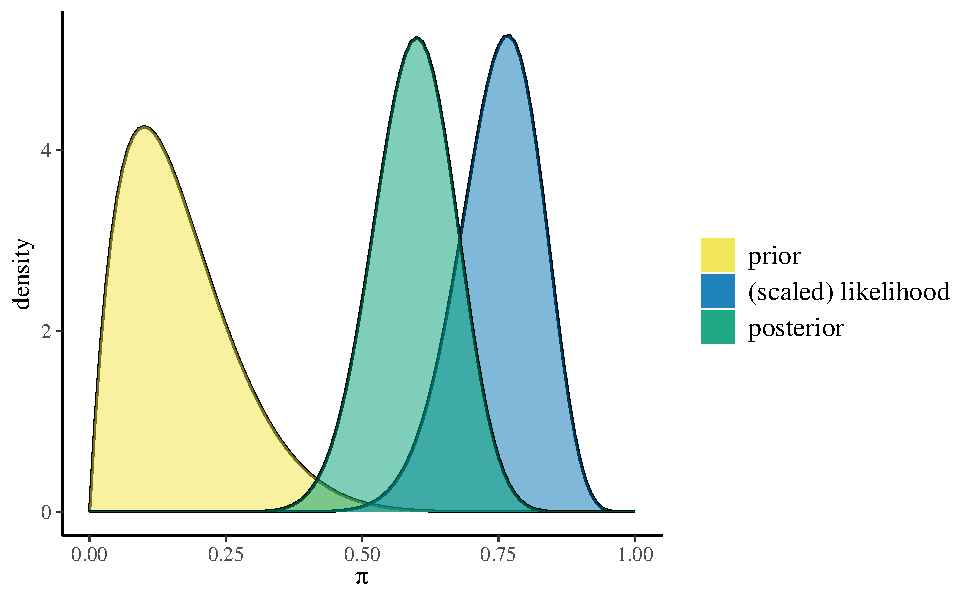
\includegraphics{ds4psy_files/figure-latex/unnamed-chunk-70-1} \end{center}

Nel modello lineare, l'osservazione \(Y_i\) è una variabile casuale, il predittore \(x_i\) è una costante fissa, e \(\beta_0\), \(\beta_1\) e \(\sigma\) sono parametri incogniti. Utilizzando il paradigma bayesiano, viene assegnata una distribuzione a priori congiunta a \((\beta_0, \beta_1, \sigma)\). Dopo avere osservato le risposte \(Y_i, i = 1, \dots, n\), l'inferenza procede stimando la distribuzione a posteriori dei parametri.

\begin{remark}

Nella costruzione di un modello di regressione bayesiano, è importante iniziare dalle basi e procedere un passo alla volta. Sia \(Y\) una variabile di risposta e sia \(x\) un predittore o un insieme di predittori. È possibile costruire un modello di regressione di \(Y\) su \(x\) applicando i seguenti principi generali:

\begin{itemize}
\item
  Stabilire se \(Y\) è discreto o continuo. Di conseguenza, identificare l'appropriata struttura dei dati (per esempio, Normale, di Poisson, o Binomiale).
\item
  Esprimere la media di \(Y\) come funzione dei predittori \(x\) (per esempio, \(\mu = \beta_0 + \beta_1 x\)).
\item
  Identificare tutti i parametri incogniti del modello (per esempio, \(\mu, \beta_1, \beta_2\)).
\item
  Valutare quali valori che ciascuno di questi parametri potrebbe assumere. Di conseguenza, identificare le distribuzioni a priori appropriate per questi parametri.
\end{itemize}

\end{remark}

Nel caso di una variabile \(Y\) continua che segue la legge gaussiana e un solo predittore, ad esempio, il modello diventa:

\begin{align} 
Y_i \mid \beta_0, \beta_1, \sigma  &\stackrel{ind}{\sim} \mathcal{N}\left(\mu_i, \sigma^2\right) \;\; \text{ con } \;\; \mu_i = \beta_0 + \beta_1 x_i \notag\\
\beta_0  &\sim \mathcal{N}\left(\mu_0, \sigma_0^2 \right)  \notag\\
\beta_1  & \sim \mathcal{N}\left(\mu_1, \sigma_1^2 \right) \notag\\
\sigma & \sim \text{Cauchy}(x_0, \gamma) \; .\notag
\end{align}

Un algoritmo MCMC viene usato per simulare i campioni dalle distribuzioni a posteriori e, mediante tali campioni, si fanno inferenze sulla risposta attesa \(\beta_0 + \beta_1 x\) per ciascuno specifico valore del predittore \(x\). Inoltre, è possibile valutare le dimensioni degli errori di previsione mediante un indice sintetico della densità a posteriori della deviazione standard \(\sigma\).

\hypertarget{considerazioni-conclusive-3}{%
\section*{Considerazioni conclusive}\label{considerazioni-conclusive-3}}


Il modello lineare semplice viene usato per descrivere la relazione tra due variabili e per determinare il segno e l'intensità di tale relazione. Inoltre, il modello lineare ci consente di prevedere il valore della variabile dipendente in base ai valori della variabile indipendente. Il modello lineare semplice è in realtà molto limitato, in quanto descrive soltanto la relazione tra la variabile dipendente \(y\) e una sola variabile esplicativa \(x\). Esso diventa molto più utile quando incorpora più variabili indipendenti. In questo secondo caso, però, i calcoli per la stima dei coefficienti del modello diventano più complicati. Abbiamo deciso di iniziare considerando il modello lineare semplice perché, in questo caso, sia la logica dell'inferenza sia le procedure di calcolo sono facilmente maneggiabili. Nel caso più generale, quello del modello lineare multiplo (ovvero, con più di un predittore), la logica dell'inferenza rimane identica a quella discussa qui, ma le procedure di calcolo richiedono l'uso dell'algebra matriciale. Il modello lineare multiplo può includere sia regressori quantitativi, sia regressori qualitativi, utilizzando un opportuno schema di codifica. È interessante notare come un modello lineare multiplo che include una sola variabile esplicativa qualitativa corrisponde all'analisi della varianza ad una via; un modello lineare multiplo che include più di una variabile esplicativa qualitativa corrisponde all'analisi della varianza più vie. Possiamo qui concludere dicendo che il modello lineare, nelle sue varie forme e varianti, costituisce la tecnica di analisi dei dati maggiormente usata in psicologia.

\mainmatter

\hypertarget{appendix-appendix}{%
\appendix \addcontentsline{toc}{chapter}{\appendixname}}


\hypertarget{simbologia-di-base}{%
\chapter{Simbologia di base}\label{simbologia-di-base}}

Per una scrittura più sintetica possono essere utilizzati alcuni simboli matematici.

\begin{itemize}
\tightlist
\item
  \(\log(x)\): il logaritmo naturale di \(x\).
\item
  L'operatore logico booleano \(\land\) significa ``e'' (congiunzione forte) mentre il connettivo di disgiunzione \(\lor\) significa ``o'' (oppure) (congiunzione debole).
\item
  Il quantificatore esistenziale \(\exists\) vuol dire ``esiste almeno un'' e indica l'esistenza di almeno una istanza del concetto/oggetto indicato. Il quantificatore esistenziale di unicità \(\exists!\) (``esiste soltanto un'') indica l'esistenza di esattamente una istanza del concetto/oggetto indicato. Il quantificatore esistenziale \(\nexists\) nega l'esistenza del concetto/oggetto indicato.
\item
  Il quantificatore universale \(\forall\) vuol dire ``per ogni.''
\item
  \(\mathcal{A, S}\): insiemi.
\item
  \(x \in A\): \(x\) è un elemento dell'insieme \(A\).
\item
  L'implicazione logica ``\(\Rightarrow\)'' significa ``implica'' (se \ldots allora). \(P \Rightarrow Q\) vuol dire che \(P\) è condizione sufficiente per la verità di \(Q\) e che \(Q\) è condizione necessaria per la verità di \(P\).
\item
  L'equivalenza matematica ``\(\iff\)'' significa ``se e solo se'' e indica una condizione necessaria e sufficiente, o corrispondenza biunivoca.
\item
  Il simbolo \(\vert\) si legge ``tale che.''
\item
  Il simbolo \(\triangleq\) (o \(:=\)) si legge ``uguale per definizione.''
\item
  Il simbolo \(\Delta\) indica la differenza fra due valori della variabile scritta a destra del simbolo.
\item
  Il simbolo \(\propto\) si legge ``proporzionale a.''
\item
  Il simbolo \(\approx\) si legge ``circa.''
\item
  Il simbolo \(\in\) della teoria degli insiemi vuol dire ``appartiene'' e indica l'appartenenza di un elemento ad un insieme. Il simbolo \(\notin\) vuol dire ``non appartiene.''
\item
  Il simbolo \(\subseteq\) si legge ``è un sottoinsieme di'' (può coincidere con l'insieme stesso). Il simbolo \(\subset\) si legge ``è un sottoinsieme proprio di.''
\item
  Il simbolo \(\#\) indica la cardinalità di un insieme.
\item
  Il simbolo \(\cap\) indica l'intersezione di due insiemi. Il simbolo \(\cup\) indica l'unione di due insiemi.
\item
  Il simbolo \(\emptyset\) indica l'insieme vuoto o evento impossibile.
\item
  In matematica, \(\mbox{argmax}\) identifica l'insieme dei punti per i quali una data funzione raggiunge il suo massimo. In altre parole, \(\mbox{argmax}_x f(x)\) è l'insieme dei valori di \(x\) per i quali \(f(x)\) raggiunge il valore più alto.
\item
  \(a, c, \alpha, \gamma\): scalari.
\item
  \(\boldsymbol{x}, \boldsymbol{y}\): vettori.
\item
  \(\boldsymbol{X}, \boldsymbol{Y}\): matrici.
\item
  \(X \sim p\): la variabile casuale \(X\) si distribuisce come \(p\).
\item
  \(p(\cdot)\): distribuzione di massa o di densità di probabilità.
\item
  \(p(y \mid \boldsymbol{x})\): la probabilità o densità di \(y\) dato \(\boldsymbol{x}\), ovvero \(p(y = \boldsymbol{Y} \mid x = \boldsymbol{X})\).
\item
  \(f(x)\): una funzione arbitraria di \(x\).
\item
  \(f(\boldsymbol{X}; \theta, \gamma)\): \(f\) è una funzione di \(\boldsymbol{X}\) con parametri \(\theta, \gamma\). Questa notazione indica che \(\boldsymbol{X}\) sono i dati che vengono passati ad un modello di parametri \(\theta, \gamma\).
\item
  \(\mathcal{N}(\mu, \sigma^2)\): distribuzione gaussiana di media \(\mu\) e varianza \(sigma^2\).
\item
  \(\mbox{Beta}(\alpha, \beta)\): distribuzione Beta di parametri \(\alpha\) e \(\beta\).
\item
  \(\mathcal{U}(a, b)\): distribuzione uniforme con limite inferiore \(a\) e limite superiore \(b\).
\item
  \(\mbox{Cauchy}(\alpha, \beta)\): distribuzione di Cauchy di parametri \(\alpha\) (posizione: media) e \(\beta\) (scala: radice quadrata della varianza).
\item
  \(\mathcal{B}(p)\): distribuzione di Bernoulli di parametro \(p\) (probabilità di successo).
\item
  \(\mbox{Bin}(n, p)\): distribuzione binomiale di parametri \(n\) (numero di prove) e \(p\) (probabilità di successo).
\item
  \(\mathbb{KL} (p \mid\mid q)\): la divergenza di Kullback-Leibler da \(p\) a \(q\).
\end{itemize}

  \bibliography{refs.bib,book.bib,packages.bib}

\printindex

\end{document}
